\documentclass[10pt]{book}
\usepackage[utf8]{inputenc}
\usepackage[italian]{babel}
\usepackage{multicol}
\usepackage[bookmarks]{hyperref}
\usepackage[a4paper, total={18cm, 25cm}]{geometry}
\usepackage{color}
\usepackage{mathrsfs}
\usepackage{amsmath}
 \usepackage{relsize}
\definecolor{mygray}{rgb}{0.5,0.5,0.5}
\usepackage{listings}
\lstset{
	language=Python,
	commentstyle=\color{mygray},
	morekeywords={function, returns, static, persistent}
}
\usepackage{graphicx}
\usepackage{makecell}
\graphicspath{ {./img/} }
\usepackage{color}
\usepackage{amssymb}

\begin{document}
\renewcommand*\contentsname{Indice}
\title{Introduzione all'Intelligenza Artificiale}
\author{Federico Matteoni}
\date{A.A. 2019/20}
\maketitle
\tableofcontents
\pagebreak
\section*{Introduzione}
Alessio Micheli, Maria Simi\\
\texttt{elearning.di.unipi.it/course/view.php?id=174}\\
Intelligenza Artificiale si occupa della \textbf{comprensione} e della \textbf{riproduzione} del comportamento \textit{intelligente}.\\
Psicologia cognitiva: obiettivo comprensione intelligenza umana, costruendo modelli computazionali e verifica sperimentale.\\
Approccio costruttivo: costruire entità dotate di intelligenze e \textbf{razionalità}. Questo tramite codifica del pensiero razionale per risolvere problemi che richiedono intelligenza non necessariamente facendolo come lo fa l'uomo.\\
Definizioni di IA: pensiero-azione, umanamente-razionalmente.\\
Costruire macchine intelligenti sia che operino come l'uomo che diversamente.\\
formalizzaz conoscenze e meccanizzazione ragionemtno in tutti i settori dell'uomo\\
comprensione tramite modelli comp della psicologia e comportamente di uomini, animali ecc\\
rendere il lavoro con il calcolatore altrettanto facile e utile che del lavoro con persone capaci, abili e disponibili.\\\\
Poniamo definizione di IA: arte di creare macchine che svolgono funzioni che richiedono intelligenza quando svolte da esseri umani. Non definisce "Intelligenza", cosa significa "intelligente"?\\

\chapter{Agenti Intelligenti}
\section{Intelligenza}
L'intelligenza è vista come l'avere diverse capacità, durante il progresso nell'area di ricerca: buon senso, interazione con un ambiente, acquisizione di esperienza, comunicazione, ragionamento logico\ldots
\paragraph{Considerazioni} L'intelligenza quindi non è una collezione di tecniche per risolvere problemi \textbf{specifici}, ma per l'informatica consiste nel \textbf{fornire metodologie sistematiche per dotare le macchine di comportamenti intelligenti/\textit{razionali} su problemi generali \textit{difficili}}.
\section{Agenti}
Iniziamo con inquadrare gli \textbf{agenti}. L'approccio moderno dell'IA consiste della costruzione di agenti intelligenti. Questa visione ci offre un quadro di riferimento ed una prospettiva \textbf{diversa} all'analisi dei sistemi software.\\
Il primo obiettivo sarà di costruire agenti per la risoluzione di problemi vista come una \textbf{ricerca in uno spazio di stati} (\textbf{problem solving})
\begin{center}
	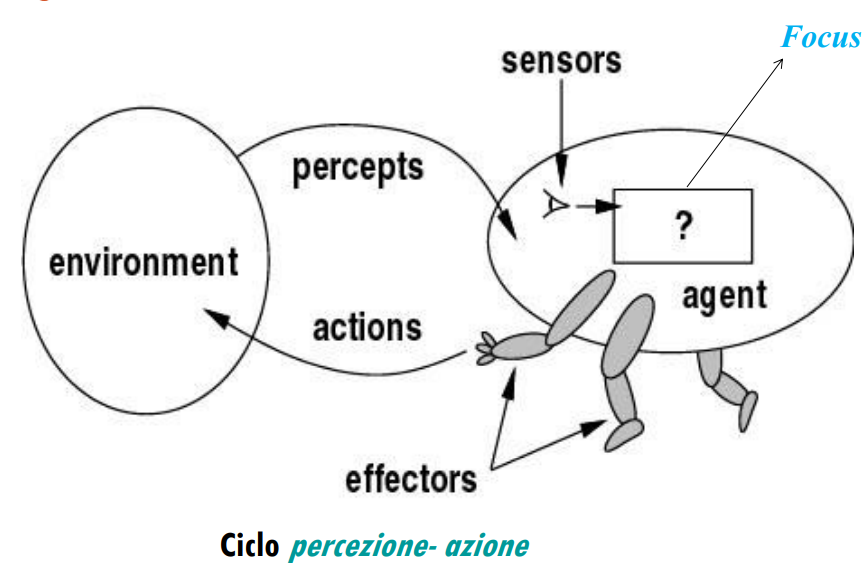
\includegraphics[scale=0.7]{agenti.png}
\end{center}
\subsection{Caratteristiche}
Sono qualcosa di più di un modulo software.
\paragraph{Situati} Gli agenti sono \textbf{situati in un ambiente} da cui \textbf{ricevono percezioni} e su cui \textbf{agiscono} mediante \textbf{azioni} (\textbf{attuatori}).
\paragraph{Sociali} Gli agenti hanno \textbf{abilità sociali}: comunicano, collaborano e si difendono da altri agenti.
\paragraph{Credenze, obiettivi, intenzioni\ldots}
\paragraph{Corpo} Gli agenti hanno un \textbf{corpo}, sono \textbf{embodied} fino a considerare i meccanismi delle emozioni.
\subsection{Percezioni e Azioni}
\paragraph{Percezione} Una percezione è un input da sensori.
\paragraph{Sequenza percettiva} Storia \textbf{completa} delle percezioni\\
La \textbf{scelta delle azioni} è \textbf{unicamente determinata dalla sequenza percettiva}.
\paragraph{Funzione Agente} Definisce l'azione da intraprendere per ogni sequenza percettiva e \textbf{descrive completamente l'agente}. Implementata da un \textbf{programma agente}.
\begin{center}
	\textbf{Sequenza Percettiva} $\longrightarrow^f$ \textbf{Azione}
\end{center}
Il compito dell'IA è progettare il programma agente.
\subsection{Agente e ambiente}
\paragraph{Architettura astratta}
\begin{center}
	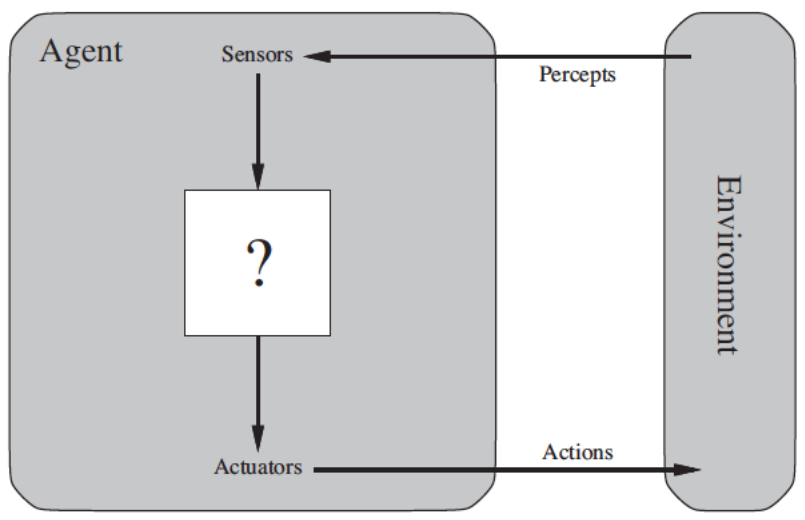
\includegraphics[scale=0.7]{ambiente.png}
\end{center}
\paragraph{Esempi}
\begin{list}{}{}
	\item \textbf{Agente robotico} Percepisce con camera, microfoni e sensori. Interagisce con motori, voce\ldots
	\item \textbf{Agente finanziario} Percepisce i tassi, le news. Interagisce con acquisti e scambi.
	\item \textbf{Agente di gioco} Percepisce le mosse dell'avversario. Interagisce tramite le proprie mosse.
	\item \textbf{Agente diagnostico} Percepisce i sintomi e le analisi dei pazienti. Interagisce fornendo la diagnosi.
	\item \textbf{Agente web} Percepisce le query utente e le pagine web. Interagisce fornendo i risultati di ricerca.
\end{list}
\subsection{Agenti Razionali}
\paragraph{Agenti razionali} Un agente razionale \textbf{interagisce con l'ambiente in maniera efficace}: "\textit{fa la cosa giusta}". L'agente razionale raggiunge l'obiettivo nella maniera più efficiente.\\
Serve quindi una \textbf{misura di prestazione}, di \textit{come vogliamo che il mondo evolva}, a seconda del problema e considerato l'ambiente.
\begin{list}{}{}
	\item \textbf{Esterna}, perché bisogna definirla \textit{prima} di agire. Non si può definire l'obiettivo dopo aver iniziato ad agire, altrimenti non è significativo.\\
	Esempio: la volpe che non arriva all'uva.
	\item Scelta dal progettista a seconda del problema e considerando l'effetto che ha sull'ambiente.
\end{list}
\paragraph{Razionalità} La razionalità è relativa/dipende da:
\begin{list}{}{}
	\item Misura delle prestazioni
	\item Conoscenze pregresse dell'ambiente
	\item Percezioni presenti e passate (sequenza percettiva)
	\item Capacità dell'agente (le azioni possibili)
\end{list}
\paragraph{Definizione} Un \textbf{agente razionale}, quindi, \textbf{esegue l'azione che massimizza il valore atteso della misura delle prestazioni per ogni sequenza di percezioni}, considerando le sue percezioni passate e la sua conoscenza pregressa.\\
Non si pretende perfezione e conoscenza del futuro, ma massimizzare il risultato \textit{atteso}. Potrebbero essere necessarie azioni di acquisizione di informazioni o esplorative (\textbf{non onniscenza}).\\
Le capacità dell'agente possono essere limitate (\textbf{non onnipotenza}).
\paragraph{Razionalità e apprendimento} Raramente il programmatore può fornire a priori tutta la conoscenza sull'ambiente. L'agente razionale, quindi, \textbf{deve essere in grado di modificare il proprio comportamento con l'esperienza}, cioè con le percezioni passate.\\
Può migliorarsi esplorando, \textbf{apprendendo}, aumentando la propria autonomia per operare in ambienti differenti o mutevoli.
\subsection{Agenti Autonomi} Un agente è \textbf{autonomo quando il suo comportamento dipende dalla sua esperienza}. Se il suo comportamento fosse determinato solo dalla propria conoscenza \textit{built-int} allora sarebbe \textbf{non autonomo} e poco flessibile.
\pagebreak
\section{Ambienti}
Definire un problema per un agente significa \textbf{caratterizzare l'ambiente in cui lavora}, cioè l'\textbf{ambiente operativo}. L'agente razionale è la soluzione del problema.
\subsection{PEAS}
\begin{list}{}{}
	\item \textbf{Performance}, prestazioni
	\item \textbf{Environment}, ambiente
	\item \textbf{Actuators}, attuatori
	\item \textbf{Sensors}, sensori
\end{list}
\paragraph{Esempio} Autista di taxi
\begin{center}
	\begin{tabular}{p{4cm} | p{4cm} | p{4cm} | p{4cm}}
		\textbf{Prestazione} & \textbf{Ambiente} & \textbf{Attuatori} & \textbf{Sensori} \\
		\hline
		Arrivare alla destinazione, sicuro, veloce, ligio alla legge, confortevole, consumo minimo di benzina, profitti massimi & Strada, altri veicoli, clienti & Sterzo, acceleratore, freni, frecce, clacson & Telecamere, sensori, GPS, contachilometri, accelerometro, sensori del motore\ldots
	\end{tabular}
\end{center}
\paragraph{Formulazione PEAS dei problemi}
\begin{center}
	\begin{tabular}{p{3cm} | p{3cm} | p{3cm} | p{3cm} | p{3cm}}
		\textbf{Problema} & \textbf{P} & \textbf{E} & \textbf{A} & \textbf{S} \\
		\hline
		Diagnosi medica & Diagnosi corretta & Pazienti, ospedale & Domande, suggerimenti, test, diagnosi & Sintomi, test clinici, risposte del paziente \\
		\hline
		Analisi immagini & Numero di immagini/zone correttamente classificate & Collezione di fotografie & Etichettatore di zone nell'immagine & Array di pixel \\
		\hline
		Robot "selezionatore" & Numero delle parti correttamente classificate & Nastro trasportatore & Raccogliere le parti e metterle nei cestini & Telecamera (pixel di varia intensità) \\
		\hline
		Giocatore di calcio & Fare più goal dell'avversario & Altri giocatore, campo di calcio, porte & Dare calci al pallone, correre & Locazione del pallone, dei giocatori e delle porte
	\end{tabular}
\end{center}
\subsection{Simulatore di Ambienti}
Uno \textbf{strumento software} con il compito di:
\begin{list}{}{}
	\item Generare gli stimoli per gli agenti
	\item Raccogliere le azioni in risposta
	\item Aggiornare lo stato dell'ambiente
	\item Opzionalmente, attivare altri processi che influenzano l'ambiente
	\item Valutare le prestazioni degli agenti
\end{list}
Gli esperimenti su classi di ambienti (variando le condizioni) sono essenziali per valutare la capacità di generalizzare. La valutazione delle prestazioni è fatta tramite la media su più istanze.
\pagebreak
\subsection{Proprietà dell'Ambiente-Problema}
\begin{list}{-}{}
	\item \textbf{Osservabilità}\\\textbf{Completamente osservabile}: l'apparato percettivo è in grado di dare una conoscenza completa dell'ambiente o almeno tutto quello che serve a decidere l'azione.\\
	\textbf{Parzialmente osservabile}: sono presenti limiti o inaccuratezze nell'apparato sensoriale. (Es. la videocamera di un rover vede solo parte dell'ambiente in un dato istante).
	\item \textbf{Singolo/Multi-Agente}\\
	Distinzione tra agente e non agente: il mondo può cambiare anche attraverso \textbf{eventi}, non necessariamente per le azioni di agenti.\\
	\textbf{Multi-Agente Competitivo}, come gli scacchi: comportamento randomizzato ma razionale.\\
	\textbf{Multi-Agente Cooperativo}, o benigno: stesso obiettivo e comunicazione.
	\item \textbf{Predicibilità}\\
	\textbf{Deterministico}: lo stato successivo è completamente determinato dallo stato corrente e dall'azione.\\
	\textbf{Stocastico}: esistono elementi di incertezza con probabilità associata. Es: guida, tiro in porta.\\
	\textbf{Non deterministico}: si tiene traccia di più stati possibili che sono risultato dell'azione, ma non in base ad una probabilità.
	\item \textbf{Episodico}: l'esperienza dell'agente è divisa in episodi atomici indipendenti. In ambienti episodici non c'è bisogno di pianificare.\\
	\textbf{Sequenziale}: ogni decisione influenza le succesive.
	\item \textbf{Statico}: il mondo non cambia mentre l'agente decide l'azione.\\
	\textbf{Dinamico}: l'ambiente cambia nel tempo, va osservata la contingenza. Tardare equivale a non agire.\\
	\textbf{Semi-dinamico}: l'ambiente non cambia ma la valutazione dell'agente si. Es: scacchi con timer, se non agisco prima dello scadere perdo.
	\item \textbf{Discreto/Continuo}\\
	Lo stato, il tempo, le percezioni e le azioni sono tutti elementi che possono assumere valori discreti o continui.\\
	Combinatoriale (nel discreto) \textit{vs} infinito (nel continuo).
	\item \textbf{Noto/Ignoto}\\
	Distinzione riferita allo stato di conoscenza dell'agente sulle leggi fisiche dell'ambiente. L'\textbf{agente conosce l'ambiente o deve compiere azioni esplorative}?\\
	\textbf{Noto $\neq$ osservabile}: posso giocare a carte coperte, ma con regole note.
\end{list}
\paragraph{Ambienti reali} Parzialmente osservabili, stocastici, sequenziali, dinamici, continui, multi-agente e ignoti.
\pagebreak

\section{Struttura di un Agente}
\begin{center}
\textbf{Agente $=$ Architettura $+$ Programma}\\
Ag: P $\longrightarrow$ Az
\end{center}
L'\textbf{Ag}ente associa \textbf{Az}ioni alle \textbf{P}ercezioni. Il \textbf{programma dell'agente} implementa la funzione \textbf{Ag}.
\paragraph{Programma Agente} Pseudocodice del programma agente.
\begin{center}
\begin{lstlisting}
function Skeleton-Agent(percept) returns action
	static: memory #la memoria del mondo posseduta dall'agente
	memory <- UpdateMemory(memory, percept)
	action <- Choose-Best-Action(memory) #Cuore dell'IA
	memory <- UpdateMemory(memory, action)
	return action
\end{lstlisting}
\end{center}
\subsection{Strutture di Agenti Caratteristici}
\paragraph{Agente basato su tabella} La scelta dell'azione è un accesso ad una tabella che \textbf{associa un'azione ad ogni possibile sequenza di percezioni}.\\
Vari \textbf{problemi}:
\begin{list}{}{}
	\item Le \textbf{dimensioni} possono essere proibitive: per giocare a scacchi, la tabella dovrebbe contenere un numero di righe nell'ordine di $10^{120} >> 10^{80}$ numero di atomi nell'universo osservabile.
	\item \textbf{Difficile da costruire}
	\item \textbf{Nessuna autonomia}
	\item \textbf{Difficile da aggiornare}, apprendimento complesso.
\end{list}
Con le IA vogliamo realizzare \textbf{automi razionali con un programma \textit{compatto}}.

\paragraph{Agente Reattivo Semplice}
\begin{center}
	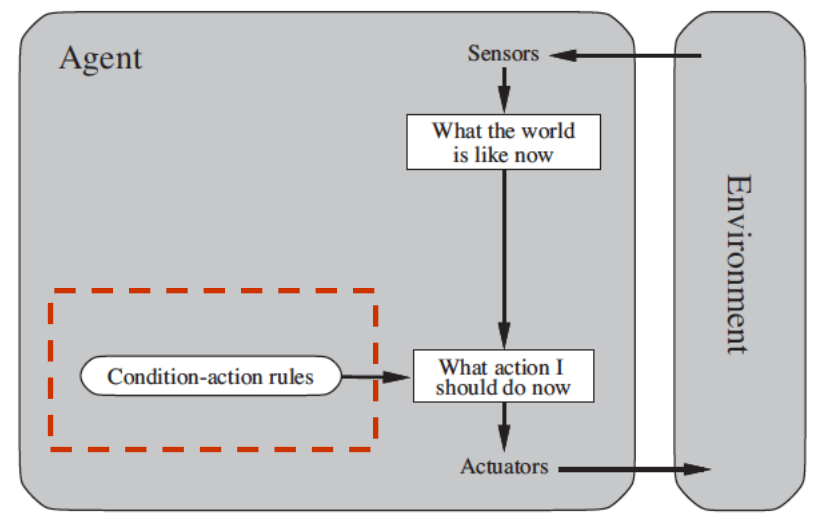
\includegraphics[scale=0.5]{agreattsemplice.png}
\end{center}
\begin{lstlisting}
function Agente-Reattivo-Semplice(percezione) returns azione
	persistent: regole #insieme di regole condizione-azione (if-then)
	stato <- Interpreta-Input(percezione)
	regola <- Regola-Corrispondente(stato, regole)
	azione <- regola.Azione
	return azione
\end{lstlisting}
\paragraph{Agenti basati su modello}
\begin{center}
	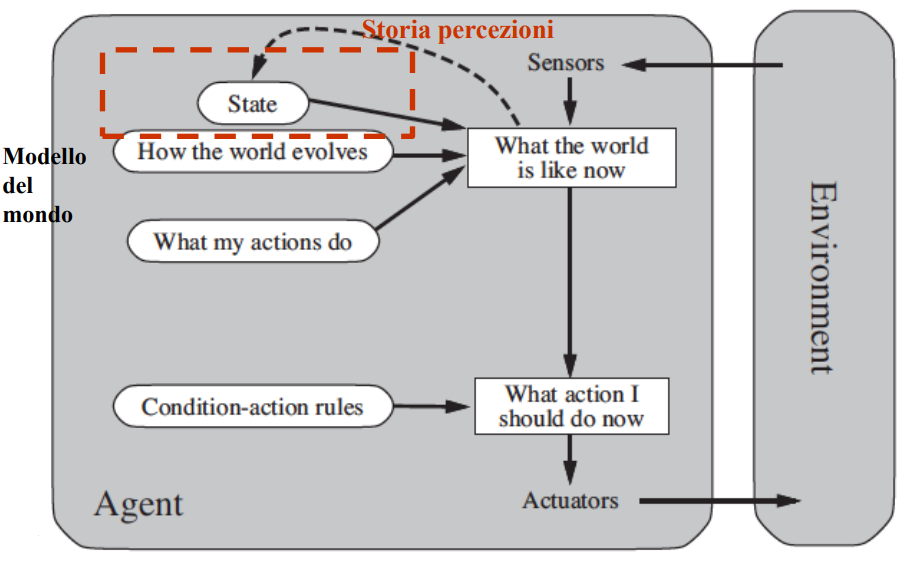
\includegraphics[scale=0.5]{agmodello.png}
\end{center}
\begin{lstlisting}
function Agente-Basato-su-Modello(percezione) returns azione
	persistent:	stato #descrizione dello stato corrente
			modello #conoscenza del mondo
			regole #insieme di regole condizione-azione
			azione #azione piu recente
	stato <- Aggiorna-Stato(stato, azione, percezione, modello)
	regola <- Regola-Corrispondente(stato, regole)
	azione <- regola.Azione
	return azione
\end{lstlisting}
\paragraph{Agenti con obiettivo} Bisogna pianificare una sequenza di azioni per raggiungere l'obiettivo. (In rosso sono indicate le parti aggiunte)
\begin{center}
	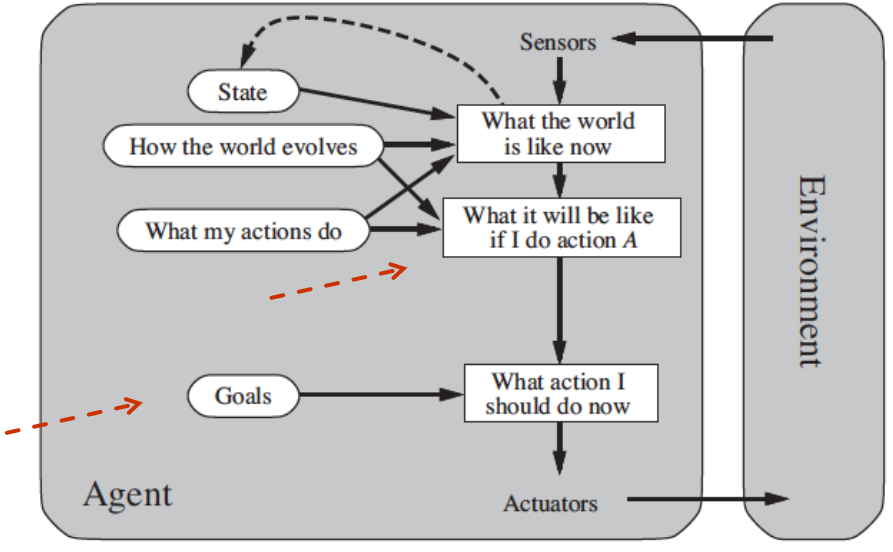
\includegraphics[scale=0.5]{agobiettivo.png}
\end{center}
Sono \textbf{guidati da un obiettivo nella scelta che intraprendono}, è stato fornito un \textbf{goal esplicito}: per esempio una città da raggiungere.\\
A volte l'azione migliore dipende dall'obiettivo da raggiungere (\textit{da che parte devo girare?})\\
Devo \textbf{pianificare una sequenza di azioni} per raggiungere l'obiettivo. Sono meno efficienti ma \textbf{più flessibili} rispetto ad un agente reattivo. L'obiettivo può cambiare, non è codificato nelle regole.\\
Esempio classico: ricerca della sequenza di azioni per raggiungere una data destinazione.
\paragraph{Agenti con valutazione di utilità}
\begin{center}
	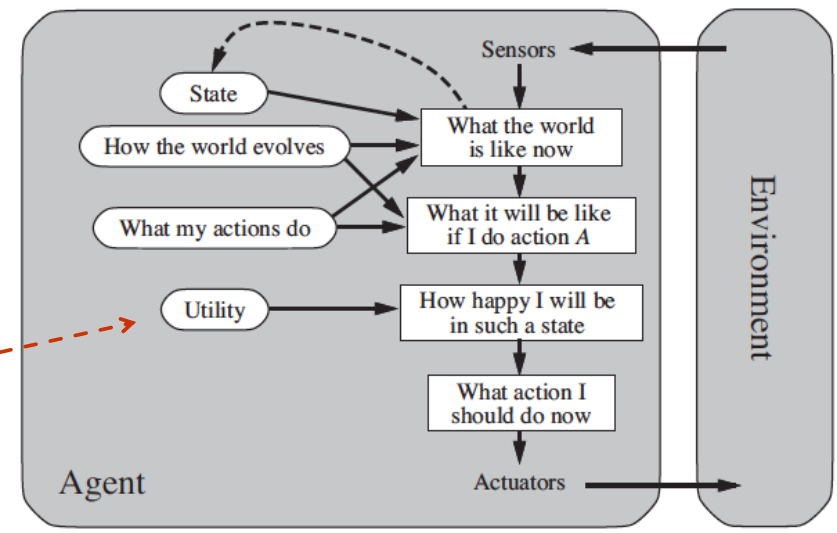
\includegraphics[scale=0.5]{agvalutazutilita.png}
\end{center}
\textbf{Obiettivi alternativi}, o più modi per raggiungerlo: l'agente deve decidere verso quali muoversi, quindi è \textbf{necessaria una funzione di utilità} che associa ad uno stato obiettivo un numero reale.\\
\textbf{Obiettivi più facilmente raggiungibili di altri}: la funzione di utilità \textbf{tiene conto della probabilità di successo} e/o di ciascun risultato (\textbf{utilità attesa} o media)
\paragraph{Agenti che apprendono}
\begin{center}
	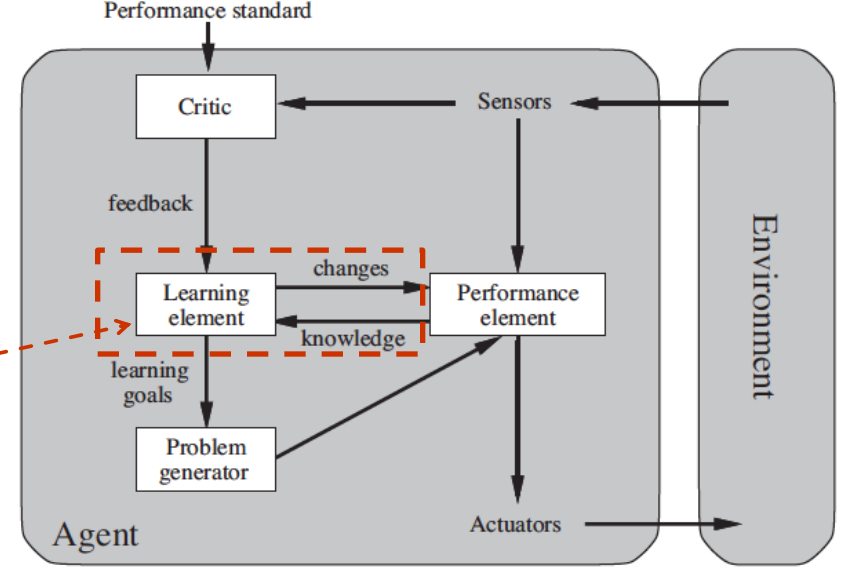
\includegraphics[scale=0.5]{agappr.png}
\end{center}
\begin{list}{}{}
	\item \textbf{Componente di apprendimento}: produce cambiamenti al programma agente. Migliora le prestazioni, adattando i suoi componenti ed apprendendo dall'ambiente
	\item \textbf{Elemento esecutivo}: il programma agente
	\item \textbf{Elemento critico}: osserva e dà feedback sul comportamento
	\item \textbf{Generatore di problemi}: suggerisce nuove situazioni da esplorare
\end{list}
\pagebreak
\subsection{Tipi di rappresentazione}
\paragraph{Stati e transizioni}
\begin{center}
	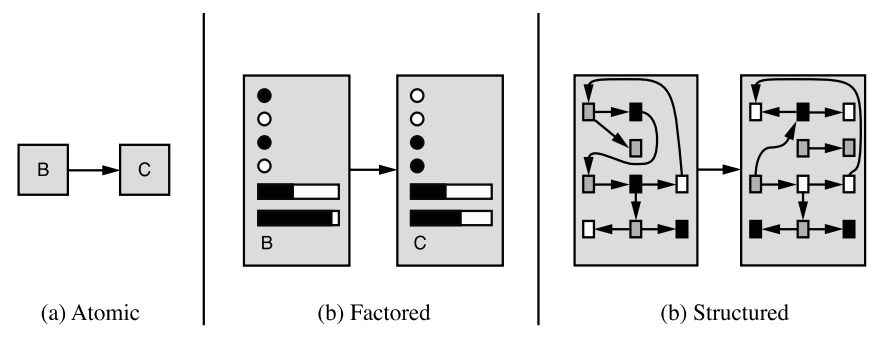
\includegraphics[scale=0.75]{rapprstatitransizioni.png}
\end{center}
\begin{list}{}{}
	\item \textbf{Rappresentazione atomica} (stati)
	\item \textbf{Rappresntazione fattorizzata} ($+$ variabili e attributi)
	\item \textbf{Rappresentazione strutturata} ($+$ relazioni)
\end{list}

\chapter{Problem Solving}
\section{Agenti Risolutori di Problemi}
\paragraph{Problem Solving} Questi agenti adottano il paradigma della \textbf{risoluzione di problemi come ricerca in uno spazio di stati} (\textbf{problemi solving}). Sono \textbf{agenti con modello} (storia, percezioni) che \textbf{adottano una rappresentazione atomica dello stato}. Sono \textbf{particolari agenti con obiettivo} che \textbf{pianificano l'intera sequenza di azioni} prima di agire.
\subsection{Processo di risoluzione}
\paragraph{Passi da seguire}
\begin{enumerate}
	\item \textbf{Determinazioni dell'obiettivo}: un insieme di stati dove l'obiettivo è soddisfatto.
	\item \textbf{Formulazione del problema}: rappresentazione degli stati e delle azioni.\\
	\textit{Fa parte del design "umano"}.
	\item \textbf{Determinazione della soluzione} mediante ricerca: un piano d'azione
	\item \textbf{Esecuzione del piano}\\
	\textit{Soluzione algoritmica}.
\end{enumerate}
La determinazione dell'obiettivo e la formulazione del problema richiede \textbf{tanta intelligenza}, che in fase di design è \textbf{spostata sull'umano}. Gli algoritmi sono ancora "\textit{stupidi}".
\paragraph{Assunzioni sull'ambiente} \textbf{Statico}, \textbf{osservabile} (so dove sono, es: \textit{viaggio con la mappa}), \textbf{discreto} (insieme finito di azioni possibili), \textbf{deterministico} (una azione $\Rightarrow$ un risultato. L'agente può eseguire il piano "\textit{ad occhi chiusi}", niente può andare storto)
\paragraph{Formulazione del problema} Un problema può essere \textbf{definito formalmente} mediante cinque componenti:
\begin{enumerate}
	\item \textbf{Stato iniziale}
	\item \textbf{Azioni possibili} nello stato \texttt{s}: \texttt{Azioni(s)}
	\item \textbf{Modello di transizione}\\
	\texttt{Risultato}: stato $\times$ azione $\longrightarrow$ stato\\
	\texttt{Risultato(s, a)}: \texttt{s'}, uno stato \textbf{successore}
	\item \textbf{Test obiettivo}: un insieme di stati obiettivo\\
	\texttt{Goal-Test}: stato $\longrightarrow$ \{\texttt{true}, \texttt{false}\}
	\item \textbf{Costo del cammino}: somma dei costi delle azioni (costo dei passi).\\
	Costo di un passo: \texttt{c(s, a, s')}, mai negativo.
\end{enumerate}
1, 2 e 3 \textbf{definiscono \textit{implicitamente} lo spazio degli stati}. Definirlo esplicitamente può essere molto oneroso, come in quasi tutti i problemi di IA.
\pagebreak
\section{Algoritmi di Ricerca}
\textit{Il processo che cerca una sequenza di azioni che raggiunge l'obiettivo è detto \textbf{ricerca}}.
\paragraph{Algoritmi} Gli algoritmi di ricerca prendono in \textbf{input un problema} e \textbf{restituiscono un cammino soluzione}, un cammino che porta dallo stato iniziale allo stato goal.
\paragraph{Misura delle prestazioni} Trova una soluzione? Quanto costa trovarla? Quanto è efficiente la soluzione?
\begin{center}
Costo Totale = Costo della Ricerca $+$ Costo del Cammino Soluzione
\end{center}
Valuteremo algoritmi sul primo, ottimizzando il secondo.
\subsection{Ricerca ad Albero}
Generazione di un \textbf{albero di ricerca sovrapposto allo spazio degli stati}. Ricerca significa \textbf{approfondire l'opzione}, mettendo da parte le altre che verranno riprese se non trovo la soluzione.\\
Quindi l'albero viene generato esplorando i vari nodi partendo dallo stato iniziale. Il nodo è diverso dallo stato: per esempio, in un grafo rappresentante le città, se parto da città A ed esploro l'opzione nodo B, il nodo B avrà come figlio anche città A perché posso tornarci.
\begin{center}
	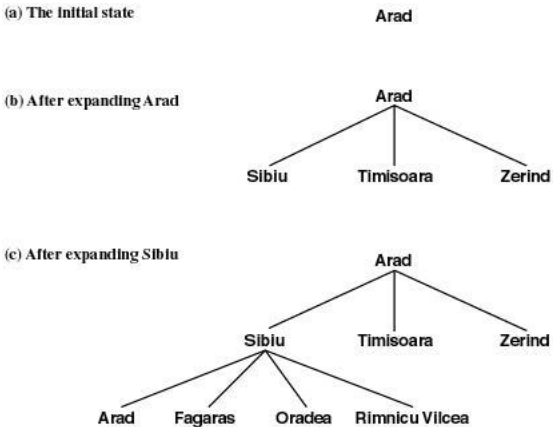
\includegraphics[scale=0.7]{ricercaalbero.png}
\end{center}
\paragraph{Algoritmo} \textbf{Ricerca ad albero}, ossia senza controllare se i nodi (\textbf{stati}) siano già stati esplorati.

\begin{lstlisting}
function Ricerca-Albero(problema) returns soluzione oppure fallimento
	#Inizializza la frontiera con stato iniziale del problema
	loop do
	if (frontiera vuota) 
		return fallimento
	#Scegli* un nodo foglia da espandere e rimuovilo dalla frontiera
	if (nodo contiene uno stato obiettivo)
		return soluzione corrispondente
	#Espandi il nodo e aggiungi i successori alla frontiera
\end{lstlisting}
$*$ $=$ \textbf{strategia}: quale scegliere? I vari algoritmi si differenziano per la strategia di scelta.\\
\begin{list}{}{Un \textbf{nodo} n è una \textbf{struttura dati con quattro componenti}}
	\item \textbf{Stato}, n.stato
	\item \textbf{Padre}, n.padre
	\item \textbf{Azione} effettuata per generarlo, n.azione
	\item \textbf{Costo} del cammino dal nodo iniziale al nodo, n.costo-cammino\\
	Indicata come g(b) = padre.costo-cammino + costo-passo ultimo)
\end{list}
\paragraph{Frontiera} Lista dei \textbf{nodi in attesa di essere espansi}, cioè \textbf{le foglie} dell'albero di ricerca. Implementata come una coda con operazioni:
\begin{list}{}{}
	\item Vuota(coda)
	\item Pop(coda) estrae l'ultimo elemento (implementa la strategia)
	\item Inserisci(elemento, coda)
\end{list}
Diversi tipi di coda hanno differenti funzioni di inserimento e \textbf{implementano strategie diverse}.
\begin{list}{}{}
	\item \textbf{FIFO} $\rightarrow$ BF\\
	Viene estratto l'elemento più vecchio, cioè in attesa da più tempo. Nuovi nodi aggiunti alla fine
	\item \textbf{LIFO} $\rightarrow$ DF\\
	Viene estratto l'ultimo elemento inserito. Nuovi nodi aggiunti all'inizio
	\item \textbf{Con priorità} $\rightarrow$ UC, altri\ldots\\
	Viene estratto l'elemento con priorità più alta in base ad una funzione di ordinamento. All'aggiunta di un nuovo nodo si riordina.
\end{list}
\paragraph{Strategie non informate}
\begin{list}{}{}
	\item Ricerca in \textbf{ampiezza} (BF)
	\item Ricerca in \textbf{profondità} (DF)
	\item Ricerca in \textbf{profondità limitata} (DL)
	\item Ricerca con \textbf{apprendimento iterativo} (ID)
	\item Ricerca di \textbf{costo uniforme} (UC)
\end{list}
\paragraph{Strategie informate} Anche dette di \textbf{ricerca euristica}: fanno uso di informazioni riguardo la distanza stimata della soluzione.
\paragraph{Valutazione di una strategia}
\begin{list}{}{}
	\item \textbf{Completezza}: se la soluzione esiste viene trovata
	\item \textbf{Ottimalità} (ammissibilità): trova la soluzione migliore, con costo minore
	\item \textbf{Complessità in tempo}: tempo richiesto per trovare la soluzione
	\item \textbf{Complessità in spazio}: memoria richiesta
\end{list}
\subsection{Breadth-First}
\paragraph{Ricerca in ampiezza} Esplorare il grafo dello spazio degli stati a livelli progressivi di stessa profondità. Implementata con una coda FIFO. \textbf{Algoritmo su albero}:
\begin{lstlisting}
function RicercaAmpiezzaA(problema)	returns soluzione oppure fallimento
	nodo = un nodo con stato = problema.stato-iniziale e costo-di-cammino = 0
	#Stati goal-tested alla generazione: maggior efficienza si ferma appena trova goal
	if (problema.TestObiettivo(nodo.Stato)) return Soluzione(nodo)
	frontiera = una coda FIFO con nodo come unico elemento
	loop do
	if (Vuota(frontiera)) return fallimento
	nodo = Pop(frontiera)
	for each azione in problema.Azioni(nodo.Stato) do #Espansione
		figlio = Nodo-Figlio(problema, nodo, azione) #costruttore: vedi AIMA
		if (Problema.TestObiettivo(figlio.Stato)) return Soluzione(figlio)
		frontiera = Inserisci(figlio, frontiera) #frontiera coda FIFO
\end{lstlisting}
\pagebreak
\textbf{Algoritmo su grafo} evitando di espandere stati già esplorati:
\begin{lstlisting}
function RicercaAmpiezzaG(problema) returns soluzione oppure fallimento
	nodo = un nodo con stato = problema.stato-iniziale e costo-di-cammino = 0
	if (problema.TestObiettivo(nodo.Stato)) return Soluzione(nodo)
	frontiera = una coda FIFO con nodo come unico elemento
	esplorati = insieme vuoto #gestisco stati ripetuti
	loop do
	if (Vuota(frontiera)) return fallimento
	nodo = POP(frontiera) #aggiungi nodo.Stato a esplorati
	for each azione in problema.Azioni(nodo.Stato) do
		figlio = Nodo-Figlio(problema, nodo, azione)
		if (figlio.Stato non in esplorati e non in frontiera)
			if (Problema.TestObiettivo(figlio.Stato)) return Soluzione(figlio)
			frontiera = Inserisci(figlio, frontiera) #in coda
\end{lstlisting}

\textbf{Python}
\begin{lstlisting}
def breadth_first_search(problem): """Ricerca-grafo in ampiezza"""
  explored = [] # insieme degli stati gia' visitati (implementato come una lista)
  node = Node(problem.initial_state) #il costo del cammino e' inizializzato nel costruttore del nodo
  if problem.goal_test(node.state):
    return node.solution(explored_set = explored)
  frontier = FIFOQueue() # la frontiera e' una coda FIFO
  frontier.insert(node)
  while not frontier.isempty(): # seleziona il nodo per l'espansione
    node = frontier.pop()
    explored.append(node.state) # inserisce il nodo nell'insieme dei nodi esplorati
    for action in problem.actions(node.state):
      child_node = node.child_node(problem,action)
      if (child_node.state not in explored) and
      (not frontier.contains_state(child_node.state)):
        if problem.goal_test(child_node.state):
        return child_node.solution(explored_set = explored)
      # se lo stato non e' uno stato obiettivo allora inserisci il nodo nella frontiera
      frontier.insert(child_node)
  return None # in questo caso ritorna con fallimento
\end{lstlisting}
\paragraph{Analisi della complessità spazio-temporale} Assumiamo:
\begin{list}{}{}
	\item \textbf{b} = fattore di ramificazione (\textbf{b}ranching)
	\item \textbf{d} = profondità del nodo obiettivo più superficiale (\textbf{d}epth)\\
	Più vicino all'iniziale
	\item \textbf{m} = lunghezza massima dei cammini nello spazio degli stati (\textbf{m}ax)
\end{list}
Analisi:
\begin{list}{}{}
	\item Strategia \textbf{completa}
	\item Strategia \textbf{ottimale} \textit{se gli operatori hanno tutti lo stesso costo k} cioè g(n) = k $\cdot$ depth(n), dove g(n) è il costo del cammino per arrivare ad n.
	\item Complessità nel tempo (nodi generati)\\
	T(b, d) = b + b$^2$ + \ldots + b$^d$ = O(b$^d$), con b figli per ogni nodo.
	\item Complessità nello spazio (nodi in memoria): O(b$^d$)
\end{list}
\pagebreak
\subsection{Depth-First}
\paragraph{Ricerca in profondità} Implementata da una coda che mette i successori in testa alla lista (LIFO, pila o stack). Algoritmo generale visto all'inizio, su grafo o albero.
\paragraph{Analisi (su albero)} Poniamo \textbf{m} lunghezza massima dei cammini nello spazio degli stati e \textbf{b} fattore di diramazione\\
Tempo: O(b$^m$) che può essere anche $>$ O(b$^d$)\\
Spazio: b$\cdot$m, frontiera sul cammino perché vengono cancellati i rami completamente esplorati ma mantenuti i fratelli del path corrente.\\
\textbf{Non completa} (loop) e \textbf{non ottimale}, ma drastico risparmio di memoria.
\begin{list}{}{}
	\item BF, d = 16 $\rightarrow$ 10 Esabyte
	\item DF, d = 16 $\rightarrow$ 156 Kilobyte
\end{list}
\paragraph{Analisi (su grafo)} In caso di DF su grafo si perdono i vantaggi di memoria: torna a tutti i possibili stati (al caso pessimo diventa esponenziale come BF) per mantenere la lista dei visitati, ma così DF diventa \textbf{completa} in spazi degli stati finiti (al caso pessimo tutti i nodi vengono espansi).\\
Rimane non completa in spazi infiniti.\\
Possibile controllare anche solo i nuovi stati rispetto al cammino radice-nodo corrente senza aggravio di memoria. Si evitano i cicli finiti in spazi finiti ma non i cammini ridondanti.
\subsection{Depth-First ricorsiva}
Ancora più efficiente in occupazione di memoria perché mantiene solo il cammino corrente (m nodi al caso pessimo).\\
Realizzata da un algoritmo ricorsivo "con backtracking" che non necessita di tenere in memoria b nodi per ogni livello, ma salva lo stato su uno stack a cui torna in caso di fallimento per fare altri tentativi. \textbf{Algoritmo su albero}:
\begin{lstlisting}
function Ricerca-DF-A (problema) returns soluzione oppure fallimento
	return Ricerca-DF-ricorsiva(CreaNodo(problema.Stato-iniziale), problema)
	
function Ricerca-DF-ricorsiva(nodo, problema) returns soluzione oppure fallimento
	if problema.TestObiettivo(nodo.Stato) return Soluzione(nodo)
	else
		for each azione in problema.Azioni(nodo.Stato) do
			figlio = Nodo-Figlio(problema, nodo, azione)
			risultato = Ricerca-DF-ricorsiva(figlio, problema)
			if risultato != fallimento then return risultato
		return fallimento
\end{lstlisting}
\textbf{Python}
\begin{lstlisting}
def recursive_depth_first_search(problem, node):  """Ricerca in profondita' ricorsiva """
  #controlla se lo stato del nodo e' uno stato obiettivo
   if problem.goal_test(node.state):
    return node.solution()
  #in caso contrario continua
  for action in problem.actions(node.state):
    child_node = node.child_node(problem, action)
    result = recursive_depth_first_search(problem, child_node)
    if result is not None: return result
  return None #con fallimento
\end{lstlisting}
\subsection{Depth-Limited}
\paragraph{Ricerca in profondità limitata} Si va in profondità fino ad un certo livello predefinito \textbf{l}.\\
\textbf{Completa} per poblemi di cui si conosce un limite superiore per la profondità della soluzione: ad esempio route-finding limitata dal numero di città - 1\\
\textbf{Completo} se d $<$ l\\
\textbf{Non ottimale}\\
Complessità in tempo: O(b$^l$)\\
Complessità in spazio: O(b$\cdot$l)
\pagebreak
\subsection{Iterative-Deepening}
\begin{center}
	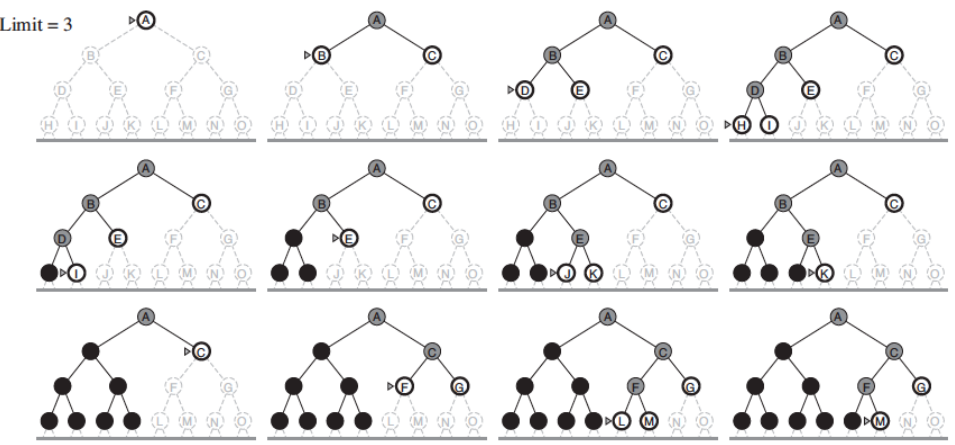
\includegraphics[scale=0.7]{id.png}
\end{center}
\paragraph{Analisi} Miglior compromesso tra BF e DF. Nell'ID, i nodi dell'ultimo livello sono generati una volta, quelli del penultimo 2, del terzultimo 3\ldots quelli del primo d volte.\\ID: (d)b + (d-1)b$^2$ + \ldots + 3b$^{d-2}$ + 2b$^{d-1}$ + b$^d$\\
Complessità in tempo: O(b$^d$)\\
Complessità in spazio: O(b$\cdot$d), vs O(b$^d$) del BF.
\section{Direzione della Ricerca}
Altro aspetto usato per ottimizzare la risoluzione di problemi, la \textbf{direzione della ricerca} è un \textbf{problema ortogonale alla strategia di ricerca}. La ricerca si può fare
\begin{list}{}{}
	\item \textbf{In avanti}, guidata dai dati come fatto fin'ora: si \textbf{esplora lo spazio di ricerca dallo stato iniziale allo stato obiettivo}
	\item \textbf{All'indietro} o \textbf{guidata dall'obiettivo}: si \textbf{esplora lo spazio di ricerca a partire da un goal e riconducendosi a sotto-goal fino a trovare uno stato iniziale}.
\end{list}
Conviene \textbf{procedere nella direzione in cui il fattore di diramazione è minore}.\\
Si preferisce la \textbf{ricerca all'indietro} quando
\begin{list}{}{}
	\item l'\textbf{obiettivo è chiaramente definito} (es. theorem proving) o si possono \textbf{formulare una serie limitata di ipotesi}
	\item i \textbf{dati del problema non sono noti} e la loro \textbf{acquisizione può essere guidata dall'obiettivo}
\end{list}
mentre si preferisce la \textbf{ricerca in avanti} quando
\begin{list}{}{}
	\item gli \textbf{obiettivi possibili sono molti} (es. design)
	\item abbiamo una \textbf{serie di dati da cui partire}
\end{list}
\pagebreak
\paragraph{Ricerca bidirezionale} Si procede nelle due direzioni fino ad incontrarsi
\begin{multicols}{2}
\begin{list}{}{}
	\item \textbf{Complessità in tempo}: O(b$^{d/2}$) = O($\sqrt{b^d}$)\\Test intersezione in tempo costante, esempio: hash table
	\item \textbf{Complessità in spazio}: O(b$^{d/2}$) = O($\sqrt{b^d}$)\\Almeno tutti i nodi in una direzione in memoria, esempio: usando BF
\end{list}
Non è sempre applicabile, ad esempio in casi di predecessori non definiti, troppi stati obiettivo\ldots
\begin{center}
	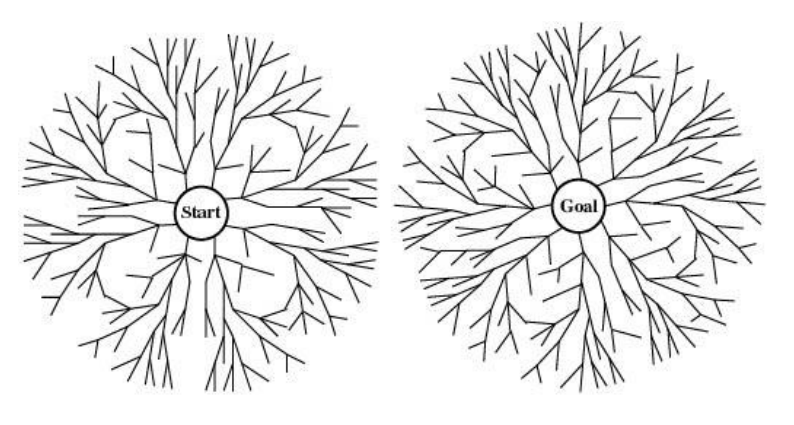
\includegraphics[scale=0.5]{ricbidirez.png}
\end{center}
\end{multicols}
\section{Problematiche}
\paragraph{Cammini Ciclici}
I \textbf{cammini ciclici} potenzialmente rendono gli alberi di ricerca infiniti, anche se con stati finiti.
\begin{center}
	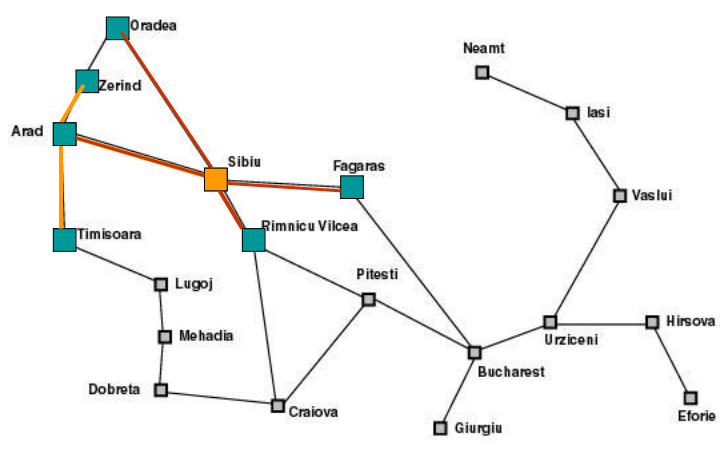
\includegraphics[scale=0.7]{camminiciclici.png}
\end{center}
\paragraph{Ridondanze}
Su spazi di stati a grafo si generano più volte nodi con lo stesso stato nella ricerca, anche in assenza di cicli.
\begin{center}
	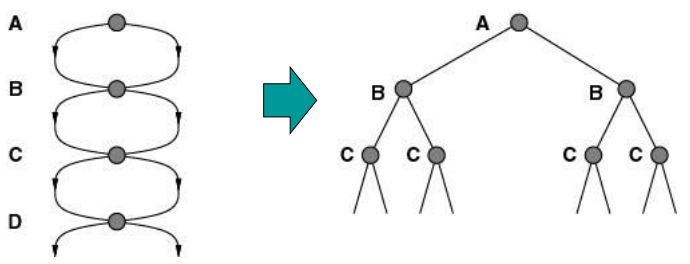
\includegraphics[scale=0.7]{ridondanze.png}
\end{center}
\pagebreak
Un caso è la \textbf{ricerca nelle griglie} Visitare stati già visitati fa compiere lavoro inutile. Costo 4$^d$ ma circa 2d$^2$ stati distinti.
\begin{center}
	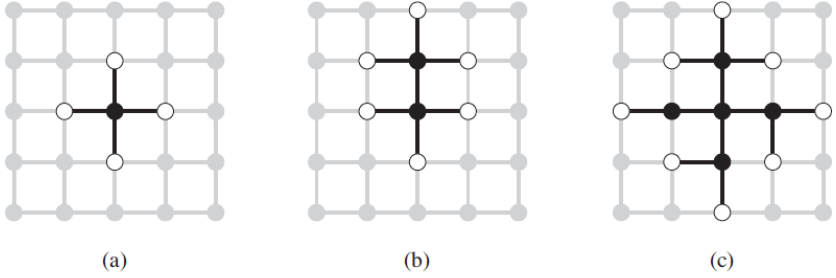
\includegraphics[scale=0.7]{griglie.png}
\end{center}
\textbf{Come evitarlo?}
\paragraph{Compromesso tra spazio e tempo} \textbf{Ricordare} gli stati visitati \textbf{occupa spazio} ma ci \textbf{consente di evitare di visitarli di nuovo}. \textit{Gli algoritmi che dimenticano la propria storia sono destinati a ripeterla}.
\subsection{Tre soluzioni} In ordine crescente di costo ed efficacia:
\begin{list}{}{}
	\item Non tornare nello stato da cui si proviene: si elimina il genitore dai nodi successori.\\
	Non evita i cammini ridondanti.
	\item Non creare cammini con cicli: si controlla che i successori non siano antenati del nodo corrente.
	\item Non generare nodi con stati già visitati/esplorati: ogni nodo visitato deve essere tenuto in memoria per una complessità O(s) dove s è il numero di stati possibili (esempio: hash table per accesso efficiente
\end{list}
\paragraph{Repetita} Il costo può essere alto: in caso di DF la memoria torna da b$\cdot$m a tutti gli stati, ma diventa una ricerca \textbf{completa} per spazi finiti. Ma \textbf{in molti casi gli stati crescono esponenzialmente} (scacchi\ldots)
\section{Uniform-Cost} \textbf{Generalizzazione della ricerca in ampiezza} (costi diversi tra passi): \textbf{si sceglie il nodo di costo g(n) del cammino minore sulla frontiera}, si espande sui contorni di uguale costo (e.g. in km) invece che sui contorni di uguale profondità (BF). Implementata da una \textbf{coda ordinata per costo cammino crescente}. \textbf{Algoritmo su albero}:
\begin{lstlisting}
function Ricerca-UC-A(problema) returns soluzione oppure fallimento
	nodo = un nodo con stato il problema.stato-iniziale e costo-di-cammino=0
	frontiera = una coda con priorita con nodo come unico elemento
	loop do
		if Vuota?(frontiera) then return fallimento
		nodo = POP(frontiera)
		#Esame post-generaz e vedere costo minore, tipico per coda con priorita
		if problema.TestObiettivo(nodo.Stato) then return Soluzione(nodo)
		for each azione in problema.Azioni(nodo.Stato) do
			figlio = Nodo-Figlio(problema, nodo, azione)
			frontiera = Inserisci(figlio, frontiera) #in coda con priorita
	end
\end{lstlisting}
\pagebreak
\textbf{Algoritmo su grafo}:
\begin{lstlisting}
function Ricerca-UC-G(problema) returns soluzione oppure fallimento
	nodo = un nodo con stato il problema.stato-iniziale e costo-di-cammino=0
	frontiera = una coda con priorita con nodo come unico elemento
	esplorati = insieme vuoto
	loop do
		if Vuota?(frontiera) then return fallimento
		nodo = POP(frontiera);
		if problema.TestObiettivo(nodo.Stato) then return Soluzione(nodo)
		aggiungi nodo.Stato a esplorati
		for each azione in problema.Azioni(nodo.Stato) do
			figlio = Nodo-Figlio(problema, nodo, azione)
			if figlio.Stato non in esplorati e non in frontiera then
				frontiera = Inserisci(figlio, frontiera) #in coda con priorita
			else if figlio.Stato in frontiera con Costo-cammino piu alto then
				sostituisci quel nodo frontiera con figlio 
\end{lstlisting}
\paragraph{Analisi} Ottimalità e completezza garantite purché il costo degli archi sia maggiore di $\epsilon > 0$. Assunto C$^*$ come il costo della soluzione ottima, allora $\lfloor$C$^*$/$\epsilon\rfloor$ \textbf{numero di mosse al caso peggiore}, arrotondato per difetto. Tendo ad andare verso tante mosse di costo $\epsilon$ prima di una che parta più alta ma poi abbia un path a costo più basso.\\
Complessità: O(b$^{1 + \lfloor C^*/\epsilon\rfloor}$).\\
Quando ogni azione ha lo stesso costo somiglia a BF ma con complessità O(b$^{1 + d}$) perché esame e arresto solo dopo aver espanso anche l'ultima frontiera.
\section{Confronto delle Strategie (albero)}
\begin{center}
\begin{tabular}{c | c | c | c | c | c | c}
Criterio & \textbf{BF} & \textbf{UC} & \textbf{DF} & \textbf{DL} & \textbf{ID} & Bidirez. \\
\hline
Completa? & Si & Si$^1$ & No & Si$^3$ & Si & Si \\
Tempo & O(b$^d$) & O(b$^{1 + \lfloor C^*/\epsilon\rfloor}$) & O(b$^m$) & O(b$^l$) & O(b$^d$) & O(b$^{d/2}$) \\
Spazio & O(b$^d$) & O(b$^{1 + \lfloor C^*/\epsilon\rfloor}$) & O(b$\cdot$m) & O(b$\cdot$l) & O(b$\cdot$d) & O(b$^{d/2}$)\\
Ottimale? & Si$^2$ & Si$^1$ & No & No & Si$^2$ & Si
\end{tabular}
\end{center}
\begin{list}{}{}
	\item $^1$ Per costi degli archi $\geq\epsilon > 0$
	\item $^2$ Se gli operatori hanno tutti lo stesso costo
	\item $^3$ Per problemi di cui si conosce un limite alla profondità della soluzione (se l $>$ d)
\end{list}
\section{Conclusioni}
Un \textbf{agente per "problem solving"} adotta un paradigma generale di risoluzione dei problemi:
\begin{list}{}{}
	\item Formula il problema, non automatico
	\item Ricerca la soluzione nello spazio degli stati, automatico
\end{list}
\chapter{Ricerca Euristica}
In problemi di complessità esponenziale, come ad es. gli scacchi ($10^{120}$ configurazioni) non è praticabile la ricerca esaustiva. Diventa quindi fondamentale \textbf{usare la conoscenza del problema e l'esperienza per riconoscere i cammini più promettenti}, evitando di generare gli altri (\textbf{pruning}).
\paragraph{Conoscenza Euristica} La \textbf{conoscenza euristica} aiuta a fare scelte oculate:
\begin{list}{}{}
	\item Non evita la ricerca, ma la riduce
	\item Consente, in genere, di trovare una \textbf{buona} soluzione in tempi accettabili
	\item Sotto certe condizioni garantisce completezza e ottimalità
\end{list}
\section{Funzione di Valutazione Euristica}
La \textbf{conoscenza} del problema è data tramite una \textbf{funzione di valutazione} $f$, che include $h$ detta \textbf{funzione di valutazione euristica}: $$h : n \rightarrow R$$
R = insieme numeri reali. La funzione si applica al nodo, ma dipende solo dallo stato (n.Stato). Per confronto, $g$ dipendeva anche dal cammino fino al nodo.
Quindi, la funzione di valutazione $$f(n) = g(n) + h(n)$$ dove g(n) è il costo del cammino visto con UC.
\paragraph{Esempio di euristica h} Per procedere preferibilmente verso il percorso migliore, seguendo il "problem-specific information", nel problema del percorso più breve da città a città posso includere nel mio algoritmo le distanze in linea d'aria, oppure il vantaggio in pezzi nella dama o negli scacchi.
\section{Best-First}
\paragraph{Algoritmo di ricerca} Best-First Heuristic utilizza lo \textbf{stesso algoritmo di Uniform-Cost} ma utilizzando f (stima di costo) per la coda con priorità. La \textbf{scelta di f determina la strategia di ricerca}: ad ogni passo si sceglie il nodo sulla frontiera per con valore di f migliore (\textbf{nodo più promettente}).
\subparagraph{Nota} Migliore significa "minore" in caso di un'euristica che stima la distanza della soluzione
\pagebreak
\subparagraph{Caso Speciale} Greedy Best-First, si usa solo h (f = h)
\begin{center}
	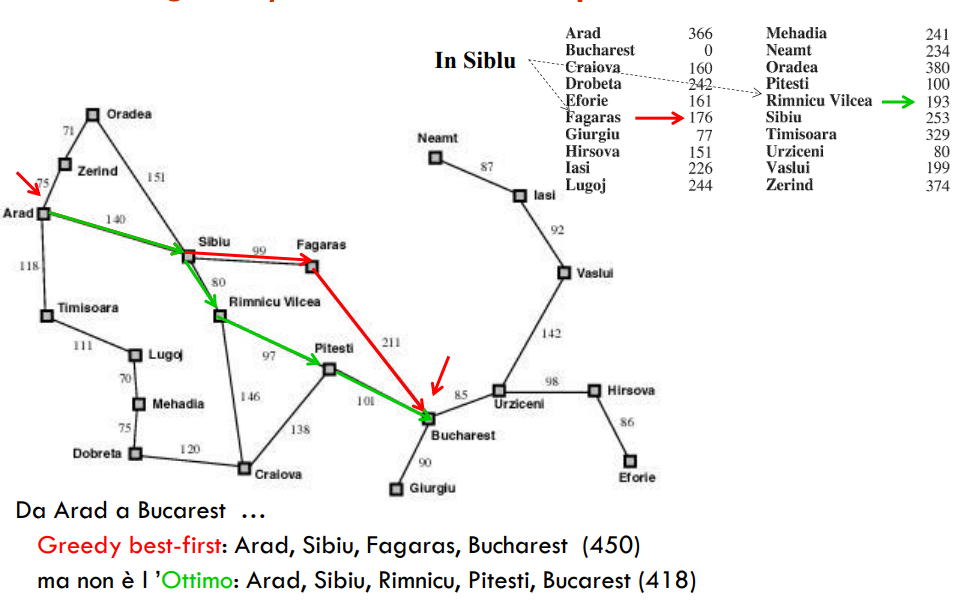
\includegraphics[scale=0.7]{greedybf.png}
\end{center}
\subsection{Algoritmo A}
Si può dire qualcosa di $f$ per avere garanzie di completezza e ottimalità?
\paragraph{Definizione} Un algoritmo A è un algoritmo Best-First con una funzione di valutazione dello stato del tipo $$f(n) = g(n) + h(n)$$ con $h(n) \geq 0$ e $h(goal) = 0$. $g(n)$ è il \textbf{costo del cammino percorso per raggiungere $n$} e $h(n)$ è \textbf{una stima del costo per raggiungere da $n$ un nodo $goal$}.
Vedremo \textbf{casi particolari} dell'algoritmo A:
\begin{list}{}{}
	\item se $h(n) = 0$, cioè $f(n) = g(n)$, si ha \textbf{Ricerca Uniforme} (UC)
	\item se $g(n) = 0$, cioè $f(n) = h(n)$, si ha \textbf{Greedy Best First}
\end{list}
\paragraph{Esempio} Il \textbf{gioco dell'otto}
\begin{multicols}{2}
\begin{center}
	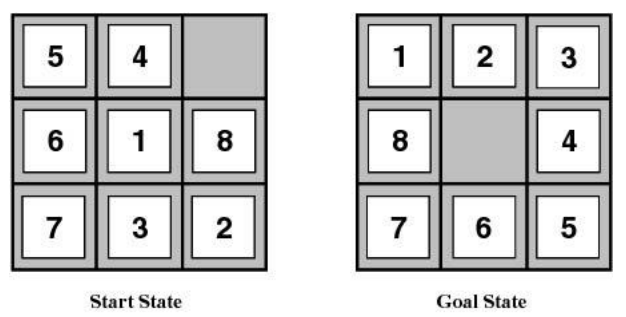
\includegraphics[scale=0.5]{8game.png}
\end{center}
\begin{list}{}{}
	\item $f(n) = $ \#mosseFatte $+$ \#caselleFuoriPosto
	\item $f(start)$ = 0 + 7\\Dopo $\leftarrow$, $\downarrow$, $\uparrow$, $\rightarrow$ si ha $f$ = 4 + 7: stesso stato ma $g$ è cambiata.
	\item $f(goal)$ = ? + 0
\end{list}
\end{multicols}
\pagebreak
\subsubsection{Algoritmo A è completo}
\paragraph{Teorema} L'algoritmo A con la condizione $g(n) \geq d(n)\cdot\epsilon$, con $d(n)$ profondità e $\epsilon > 0$ costo minimo dell'arco, è \textbf{completo}.\\
La condizione ci garantisce che non si verifichino condizioni del tipo
\begin{center}
	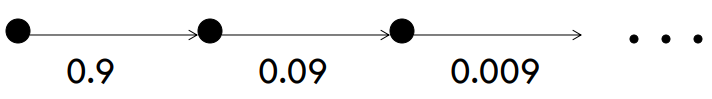
\includegraphics[scale=0.5]{complA.png}
\end{center}
e che il costo lungo un cammino non cresca "abbastanza", così da fermarsi per costi alti di $g$.
\paragraph{Dimostrazione} Sia $[n_0\:n_1\:n_2 \ldots\:n'\:\ldots\:n_k = goal]$ un cammino soluzione. Sia $n'$ un nodo della frontiera su un cammino soluzione $\rightarrow$ $n'$ prima o poi \textbf{verrà espanso}. Infatti, esistono solo un numero finito di nodi $x$ che possono essere aggiunti alla frontiera con $f(x) \leq f(n')$ (condizione su $g$).\\
Quindi, se non si trova una soluzione prima, $n'$ verrà espanso e i suoi successori aggiunti alla frontiera. Tra questi, \textbf{anche il suo successore sul cammino soluzione}.\\
Il ragionamento si può ripetere fino a dimostrare che anche il nostro $goal$ sarà selezionato per l'espansione.
\subsection{Algoritmo A*: La Stima Ideale}
Una \textbf{funzione di valutazione ideale} (\textbf{oracolo}) $f^*(n) = g^*(n) + h^*(n)$
\begin{list}{}{}
	\item $g^*(n)$ costo del \textbf{cammino minimo} da radice a $n$
	\item $h^*(n)$ costo del \textbf{cammino minimo} da $n$ a $goal$
	\item $f^*(n)$ costo del \textbf{cammino minimo} da radice a $goal$, attraverso $n$
\end{list}
Normalmente $g(n) \geq g^*(n)$ (costo del cammino $\geq$ cammino minimo) e $h(n)$ è una \textbf{stima} di $h^*(n)$: si può sotto o sovrastimare la distanza dalla soluzione.
\paragraph{Definizione} \textbf{Euristica ammissibile} $\forall n \:\:\vline\:\:h(n) \leq h^*(n)$, $h$ è una \textbf{sottostima}, ad esempio l'euristica della distanza in linea d'aria.
\paragraph{Definizione} Algoritmo A*: un algortimo A in cui $h$ è una funzione euristica ammissibile.
\paragraph{Teorema} Gli algoritmi A* sono \textbf{ottimali}.
\paragraph{Corollario} BF con passi a costo costante e UC sono \textbf{ottimali} ($h(n) = 0$)
\begin{center}
	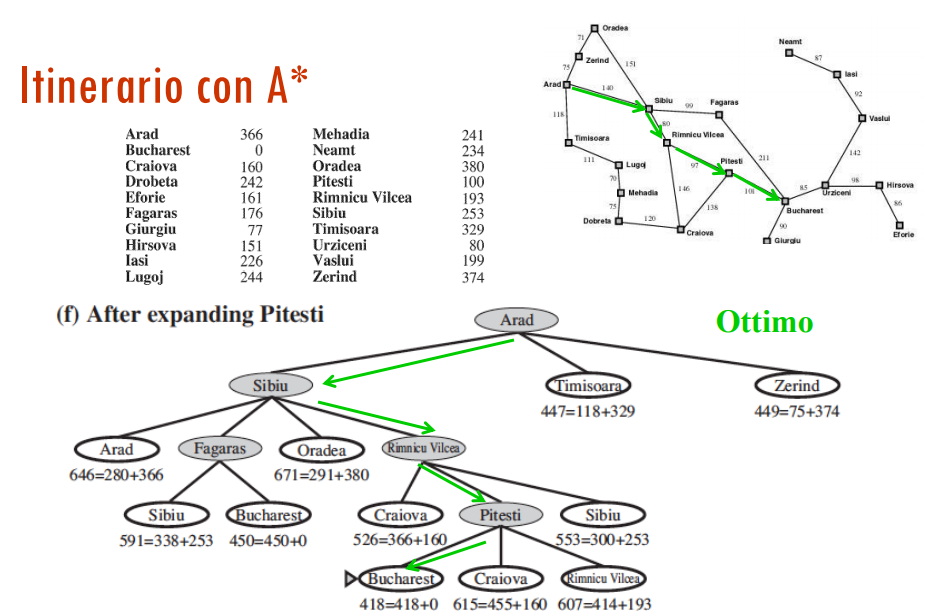
\includegraphics[scale=0.5]{itAstar.png}
\end{center}
\pagebreak
\paragraph{Osservazioni} La componente $g$ fa sì che si abbandonino cammini che vanno troppo in profondità.\\
\textbf{$h$ sotto o sovra stima}? Una sottostima può farci compiere lavoro inutile, ma \textbf{non fa perdere il cammino migliore}: quando trovo il nodo $goal$ è il cammino migliore. Invece, una funzione che a volte sovrastima può \textbf{farci perdere la soluzione ottimale a causa di tagli per sovrastima}.
\paragraph{Ottimalità} Nel caso di ricerca su ablero, l'\textbf{uso di un'euristica ammissibile è sufficiente a garantire l'ammissibilità} $\Rightarrow$ \textbf{ottimalità di A*}.\\
Nel caso di ricerca su grafo, serve una proprietà più forte: la \textbf{consistenza}, anche detta \textbf{monotonicità}, perché rischio di scartare candidati ottimi (stato già incontrato) a meno che il primo espanso sia il migliore.
\paragraph{Definizione} \textbf{Euristica consistente} se
\begin{list}{}{}
	\item $h(goal) = 0$
	\item \textbf{Consistenza locale}: $\forall n\:\:\vline\:\:h(b) \leq c(n, a, n') + h(n')$ dove $n'$ è un successore di $n$ e $c(n, a, n')$ è il costo del cammino $n\rightarrow n'$ sull'arco $a$.
	\item $\Rightarrow$ $f(b) \leq f(n')$
\end{list}
Quindi se $h$ è consistente, allora \textbf{$f$ non decresce mai lungo i cammini}: da qui il termine monotonia.\\
Esistono euristiche ammissibili che non sono monotone, ma sono rare.
\paragraph{Teorema} Un'\textbf{euristica monotona è ammissibile}.\\
Le euristiche monotone garantiscono che la \textbf{soluzione meno costosa venga trovata per prima} e quindi \textbf{sono ottimali anche nel caso di ricerca su grafo}.
\begin{list}{}{}
	\item Non si devono recuperare, tra gli antenati, nodi con costo minore
	\item \textbf{Lista degli esplorati}, stato già esplorato è sul cammino ottimo $\Rightarrow$ posso evitare di inserire il corrente ripetuto senza perdere l'ottimalità
	\begin{lstlisting}
	if (figlio.Stato non in Esplorati and non in Frontiera)
		Frontiera = Inserisci(figlio, Frontiera)
	\end{lstlisting}
	\item Per la frontiera, volendo evitare stati ripetuti, resta l'\texttt{if} finale di UC
	\begin{lstlisting}
	if (figlio.Stato in Frontiera con costoCammino piu alto)
		sostituisci quel nodo frontiera con il figlio
	\end{lstlisting}
\end{list}
\paragraph{Ottimalità di A*} \textbf{Dimostrazione}\\
\textbf{1.} $h(n)$ consistente $\Rightarrow$ i valori di $f(n)$ lungo un cammino sono non decrescenti:
\begin{list}{}{}
	\item Se $h(n) \leq c(n, a, n’) + h(n’)$ (def. consistenza)
	\item $g(n) + h(n) \leq g(n) + c(n, a, n’) + h(n’)$ sommando g(n)
	\item ma siccome $g(n) + c(n, a, n’) = g(n’)$, allora $g(n) + h(n) \leq g(n’) + h(n’)$
	\item quindi $f(n) \leq f(n’)$
\end{list}
\textbf{2.} Ogni volta che A* seleziona un nodo $n$ per l’espansione, il
cammino ottimo a tale nodo è stato trovato.\\
Se così non fosse, ci sarebbe un altro nodo $n’$ della frontiera sul cammino ottimo (a $n$, ancora da trovare), con $f(n’)$ minore (per la monotonia e n successivo di $n’$).\\
Ma ciò non è possibile perché tale nodo sarebbe già stato espanso.\\\\
\textbf{3.} Quando seleziona nodo $goal$ è cammino ottimo $[h=0, f=C^*]$
\subsection{Perché A* è vantaggioso?}
\begin{list}{}{}
	\item A* espande tutti i nodi con $f(n) < C^*$
	\item A* espande \textit{alcuni} nodi con $f(n) = C^*$
	\item \textbf{A* non espande alcun nodo con $f(b) > C^*$}
\end{list}
Quindi alcuni nodi (e suoi sottoalberi) non verranno considerati per l'espansione, ma restiamo ottimali: \textbf{pruning}, un'$h$ opportuna, \textbf{più alta possibile fra le ammissibili}, fa tagliare molto.
\pagebreak
\begin{center}
	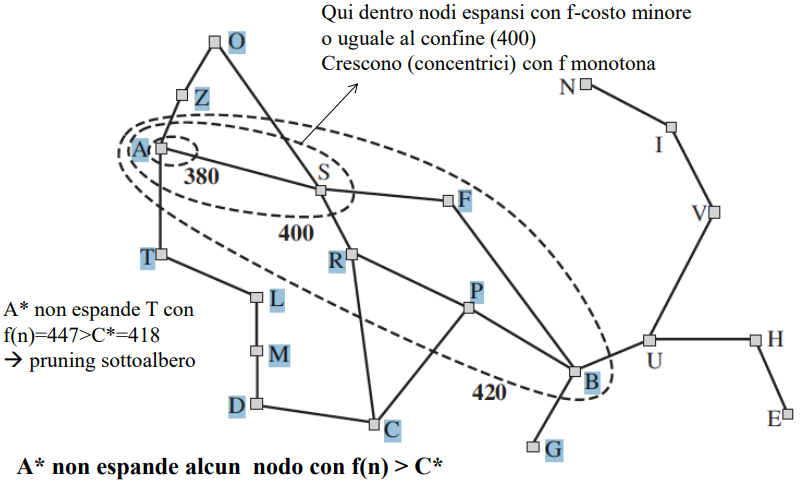
\includegraphics[scale=0.7]{astarcontorni.png}
\end{center}
Più $f$ è aderente, più taglio ottenendo ovali più stretti. Cercheremo quindi un'$h$ \textbf{più alta possibile tra le ammissibili}. Se molto bassa, molti (sino a tutti) nodi restano $< C^*$ $\Rightarrow$ espando tutti (a cerchi).
\paragraph{Pruning} Il \textbf{pruning dei sotto-alberi è il punto focale}: non li abbiamo già in memoria ed \textbf{evitiamo di generarli}, e ciò è \textbf{decisivo per i problemi di AI a spazio stati esponenziali}.
\subsection{Conslusioni su A*}
\paragraph{Algoritmo} Lo stesso usato per UC
\paragraph{Funzioni} Usa $f = g + h$ per la coda di priorità, dove $h$ e $g$ soddisfano le condizioni per algoritmo A e $h$ è una funzione euristica ammissibile per A*.\\
Sui grafi necessità di un'euristica monotona.
\paragraph{Completo} Discende dalla completezza di A, perché A* è un A particolare
\paragraph{Ottimale} Con euristica monotona
\paragraph{Ottimamente efficiente} A parità di euristica nessun'altro algoritmo espande meno nodi senza rinunciare ad ottimalità
\paragraph{Problemi} Quale euristica?\\
Occupazione in memoria: O(b$^{d+1}$)
\subsection{Casi speciali di A}
\begin{list}{}{}
	\item $h(n) = 0$ si ha Uniform Cost, cioè $f(n) = g(n)$\\
	Cioè $g$ non basta
	\item $g(n) = 0$ si ha Greedy Best First, cioè $f(n) = h(n)$\\
	Ossia $h$ non basta
\end{list}
\pagebreak
\section{Costruire le Euristiche di A*}
\subsection{Valutazione di funzioni euristiche}
A parità di ammissibilità, \textbf{una euristica può essere più efficiente di un'altra} nel trovare il cammino soluzione migliore. Questo \textbf{dipende da quanto \textit{informata} è l'euristica}, cioè dal \textbf{grado di informazione posseduto}.
\begin{list}{}{}
	\item $h(n) = 0$ \textbf{minimo} di informazione (BF, o UC)
	\item $h^*(n)$ \textbf{massimo} di informazione (oracolo)
\end{list}
In generale, per le euristiche ammissibili, $$0 \leq h(n) \leq h^*(n)$$
\paragraph{Teorema} Se $h_1 \leq h_2$, i nodi espansi da A* con $h_2$ sono un \textbf{sottoinsieme} di quelli espansi da A* con $h_1$.\\
Questo perché A* espande tutti i nodi con $f(n) < C^*$ e sono meno per $h$ maggiore (fa andare più nodi oltre $C^*$).\\
$\Rightarrow$ Se $h_1 \leq h_2$, allora A* con $h_2$ è \textbf{almeno efficiente} quanto A* con $h_1$.\\\\
Un'euristica più informata (accurata) riduce lo spazio di ricerca (più efficiente) ma è tipicamente \textbf{più costosa da calcolare}.
\subsection{Confronto di euristiche ammissibili}
\paragraph{Esempio} Due euristiche ammissibili per il gioco dell'otto
\begin{list}{}{}
	\item $h_1$ conta il numero di caselle fuori posto
	\item $h_2$ somma delle distanze Manhattan (orizz/vert) delle caselle fuori posto dalla posizione finale\\
	Manhattan Distance: $h(x, y) = MD((x, y), (x_g, y_g)) = |x - x_g| + |y - y_g|$
\end{list}
$\Rightarrow$ $h_2$ è \textbf{più informata} di $h_1$, infatti $\forall n \Rightarrow h_1(n) \leq h_2(n)$. Si dice che \textbf{$h_2$ domina $h_1$}.
\begin{center}
	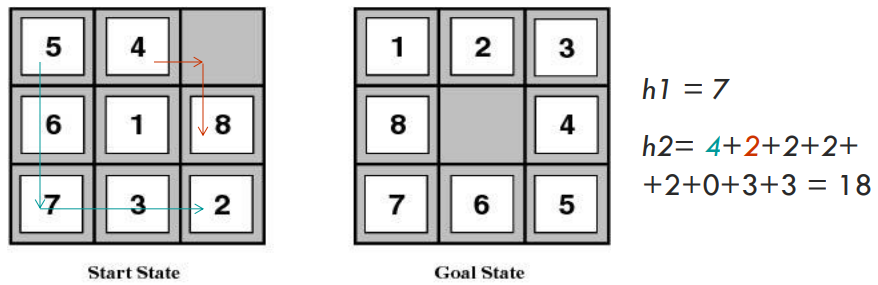
\includegraphics[scale=0.7]{confrh.png}
\end{center}
\subsection{Misura del potere euristico}
Come valutare gli algoritmi di ricerca euristica
\paragraph{Fattore di diramazione effettivo} Dato N numero di nodi generati, d profondità della soluzione, allora b* è il \textbf{fattore di diramazione di un albero uniforme con N+1 nodi}, soluzione dell'equazione $$N + 1 = b^* + (b^*)^2 + \ldots + (b^*)^d$$ Sperimentalmente, una buona euristica ha un b* abbastanza vicino ad 1 ($<$ 1.5)
\paragraph{Esempio} $d = 5,\:\: N = 52 \Rightarrow b^* = 1.92$
\pagebreak
\subsection{Capacità di esplorazione} Influenza di b*
\begin{multicols}{2}
	\begin{list}{}{Con $b = 2$}
		\item $d = 6\:\:\:\:N = 100$
		\item $d = 12\:\:N = 10000$
	\end{list}
		\begin{list}{}{Con $b = 1.5$}
		\item $d = 12\:\:N = 100$
		\item $d = 24\:\:N = 10000$
	\end{list}
\end{multicols}
Quindi \textbf{migliorando di poco l'euristica si riesce, a parità di nodi espansi, a raggiungere una profondità doppia}.
\subsection*{Quindi}
Tutti i problemi dell'IA, o quasi, sono di complessità esponenziale nel generare nodi (ad es. configurazioni possibili), ma c'è esponenziale ed esponenziale. L'euristica può migliorare di molto la capacità di esplorazione dello spazio degli stati rispetto alla ricerca cieca: \textbf{migliorando anche di poco l'euristica si riesce ad esplorare uno spazio molto più grande}.
\section{Come si inventa un'euristica?}
Alcune strategie per ottenere euristiche ammissibili, da vedere man mano:
\begin{list}{}{}
	\item \textbf{Rilassamento} del problema
	\item \textbf{Massimizzazione di euristiche}
	\item \textbf{Database di pattern disgiunti}
	\item \textbf{Combinazione lineare}
	\item \textbf{Apprendere} dall'esperienza
\end{list}
\subsection{Rilassamento del problema}
\textbf{Spazio degli stati con archi aggiunti}.
\paragraph{Gioco dell'otto} Nel gioco dell'otto, mossa da A a B possibile se \textbf{B adiacente ad A} e \textbf{B libera}.\\
$h_1$ e $h_2$ sono \textbf{calcoli della distanza esatta della soluzione} in \textbf{versioni semplificate} del puzzle: uno \textbf{spazio degli stati con archi aggiunti}
\begin{list}{}{}
	\item $h_1$ nessuna restrizione: sono sempre ammessi scambi tra caselle, si muove ovunque $\rightarrow$ numero di caselle fuori posto
	\item $h_2$ solo prima restrizione: sono ammessi spostamenti anche su caselle occupate purché adiacenti $\rightarrow$ somma delle distanze Manhattan
\end{list}
\subsection{Massimizzazione di euristiche}
Si hanno una serie di euristiche ammissibili $h_1$, $h_2$, \ldots, $h_k$, \textbf{senza che nessuna domini un'altra}. Allora conviene \textbf{prendere il massimo dei loro valori} $$h(n) = max\{h_1(n),\:\:h_2(n),\:\:\ldots,\:\:h_k(n)\}$$ Se le $h_i$ sono ammissibili, anche la $h$ lo è e \textbf{domina tutte le altre}.
\pagebreak
\paragraph{Euristiche da sottoproblemi}
\begin{center}
	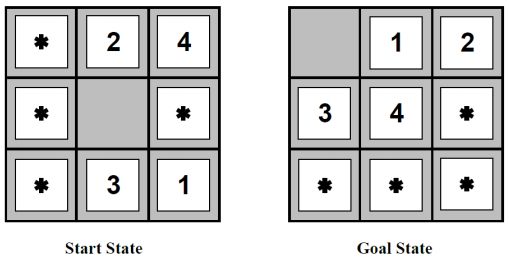
\includegraphics[scale=0.7]{eursottoprob.png}
\end{center}
Il \textbf{costo della soluzione ottima del sottoproblema} (sistemare 1, 2, 3, 4) è una \textbf{sottostima del costo del problema nel suo complesso} e più accurata della Manhattan.\\
\textbf{Database di pattern}: si \textbf{memorizza ogni istanza del sottoproblema con relativo costo} della soluzione. Si usa il \textbf{database per calcolare $h_{DB}$}, estraendo dal DB la configurazione corrispondente allo stato completo corrente.
\paragraph{Sottoproblemi multipli} Potremmo poi fare la stessa cosa per altri sottoproblemi: 5-6-7-8, 2-4-6-8\ldots ottenendo altre euristiche ammissibili.\\
Poi si può prendere il valore massimo: altra euristica ammissibile.\\
Ma potremmo sommarle ed ottenere un'euristica ancora più accurata?
\subsection{Pattern Disgiunti} In generale no, perché le \textbf{soluzioni ai sottoproblemi interferiscono}: nel caso del gioco dell'otto, condividono alcune mosse perché se sposto 1-2-3-4 sposto anche 4-5-6-7.\\
La \textbf{somma delle euristiche in generale non è ammissibile} perché potremmo sovrastimare, avendo avuto aiuti mutui.\\
Si deve \textbf{eliminare il costo delle mosse che contribuiscono all'altro sottoproblema}: \textbf{databse di \textit{pattern disgiunti}} consentono di sommare i costi (\textbf{euristiche additive}).\\
Sono molto efficaci: gioco del 15 in pochi ms. Ma difficile scomporre per il cubo di Rubik.
\subsection{Apprendere dall'esperienza}
Si fa girare il programma e si raccolgono i dati sottoforma di \textbf{coppie} \texttt{<stato, h*>}. Si usano i dati per apprendere come predire la $h$ con \textbf{algoritmi di apprendimento induttivo}: da istanze note stimiamo $h$ \textbf{in generale}.\\
Gli algoritmi di apprendimento si concentrano su caratteristiche salienti dello stato (\textit{feature}, $x_i$). Esempio: numero tasselli fuori posto 5 $\rightarrow$ costo 14.
\subsubsection{Combinazione di euristiche}
Quando diverse caratteristiche influenzano la bontà di uno stato, si può usare una combinazione lineare $$h(n)= c_1 x_1(n) + c_2 x_2(n) + \ldots + c_k x_k(n)$$
Gioco dell'otto $h(n) = c_1 \#fuoriPosto + c_2 \#coppieScambiate$\\
Scacchi $h(n) = c_1 vantaggioPezzi + c_2 pezziAttaccante + c_3 regina + \ldots$\\
Il \textbf{peso dei coefficienti può essere aggiustato con l'esperienza}, anche qui \textbf{apprendendo automaticamente da esempi di gioco}. $h(goal) = 0$ ma ammissibilità e consistenza \textbf{non} automatiche.

\chapter{Algoritmi Evolutivi Basati su A*}
\section{Beam Search}
Nel \textbf{best first} viene mantenuta tutta la frontiera. Se l'occupazione di memoria è eccessiva, si può ricorrere ad una variante: la \textbf{beam search}.
\paragraph{Beam Search} La beam search \textbf{tiene ad ogni passo solo i $k$ nodi più promettenti}, dove $k$ è detto \textbf{ampiezza del raggio} (beam).\\
\textbf{Non è completa}.
\section{IDA*}
A* con approfondimento iterativo. IDA* combina A* con ID: ad ogni iterazione si ricerca in profondità con un limite (cut-off) dato dal valore della funzione $f$ (e non dalla profondità).\\
Il limite \textbf{f-limit} viene aumentato ad ogni iterazione, fino a trovare la soluzione.
\paragraph{Punto Critico} Di quanto viene aumentato f-limit.
\paragraph{Quale incremento?} Cruciale la scelta dell'incremento per garantire l'ottimalità. In caso di azioni dal costo fisso, il limite viene incrementato dal costo delle azioni.\\
Ma in caso di costi variabili? Costo minimo? Si potrebbe, ad ogni passo, fissare il limite successivo al valore minimo delle $f$ scartate (in quanto superavano il limite) all'interazione precedente.
\paragraph{Analisi} \textbf{Completo} e \textbf{ottimale}. Occupazione in memoria O(bd).
\section{RBFS}
Best-First Ricorsivo: simile a DF ricorsivo ma cerca di usare meno memoria, facendo del lavoro in più.\\
Tiene traccia del migliore percorso alternativo ad ogni livello. Invece di fare backtracking in caso di fallimento, interrompe l’esplorazione quando trova un nodo meno promettente secondo $f$. Nel tornare indietro \textbf{si ricorda il miglior nodo che ha
trovato nel sottoalbero esplorato}, per poterci eventualmente tornare\\
Memoria: lineare nella profondità della soluzione ottima.
\section{A* con memoria limitata}
L'idea è quella di utilizzare al meglio la memoria disponibile.\\
SMA* procede come A* fino ad esaurimento della memoria disponibile. A questo punto “dimentica” il nodo peggiore, dopo avere aggiornato il valore del padre.\\
A parità di $f$ \textbf{si sceglie il nodo migliore più recente e si dimentica il nodo peggiore più vecchio}.\\
\textbf{Ottimale se il cammino soluzione sta in memoria}.\\
\pagebreak

In algoritmi a memoria limitata, le limitazioni della memoria possono portare a compiere molto lavoro inutile: ad esempio, visitare ripetutamente gli stessi nodi. Diventa quindi \textbf{difficile stimare la complessità temporale effettiva}. Le \textbf{limitazioni della memoria}, quind, \textbf{possono rendere un problema intrattabile} dal punto di vista computazionale.
\section{Conclusioni}
\begin{list}{}{}
	\item \textbf{Agenti} in \textbf{ambienti deterministici}, \textbf{osservabili}, \textbf{statici} e \textbf{completamente noti}
	\item \textbf{Ricerca} come \textbf{scelta della sequenza di azioni}, cioè cammino in uno spazio di stati, \textbf{che raggiunge obiettivo} $\Rightarrow$ il cammino è la soluzione
	\item \textbf{Attività necessarie}
	\begin{list}{}{}
		\item Formulazione del problema
		\item Scelta dell'algoritmo di ricerca adeguato
		\item Identificazione della funzione di valutazione euristica più efficace
	\end{list}
\end{list}
\chapter{Oltre la Ricerca Classica}
\paragraph{Risolutori "classici"} Gli agenti risolutori di problemi \textit{classici} assumono le condizioni viste in precedenza:
\begin{list}{}{}
	\item Ambienti completamente osservabili
	\item Ambienti deterministici
	\item Si trovano nelle condizioni di produrre un piano d'azione eseguibile "ad occhi chiusi": possono studiare la sequenza d'azioni \textit{offline}, che può essere eseguita senza imprevisti per raggiungere l'obiettivo
\end{list}
\section{Verso ambienti più realistici} La \textbf{ricerca sistematica}, o euristica, nello spazio di stati è \textbf{troppo costosa} $\longrightarrow$ Metodi di ricerca locale\\
Assunzioni sull'ambiente da considerare:
\begin{list}{}{}
	\item \textbf{Azioni non deterministiche}\\
	\textbf{Ambiente parzialmente osservabile}\\
	$\longrightarrow$ Piani condizionali, ricerca \texttt{AND-OR}, stati credenza
	\item \textbf{Ambienti sconosciuti}\\
	\textbf{Problemi di esplorazione} (percezioni forniscono nuove informazioni dopo l'azione)\\
	$\longrightarrow$ Ricerca \textbf{online}
\end{list}
\section{Ricerca Locale}
\paragraph{Assunzioni}
Gli algoritmi visti fin'ora esplorano gli spazi degli stati alla ricerca di un goal e restituiscono un \textbf{cammino soluzione}, ma \textbf{a volte lo stato goal è la soluzione} del problema. Gli \textbf{algoritmi di ricerca locale} sono adatti per problemi in cui
\begin{list}{}{}
	\item La sequenza di azioni non è importante: quello che conta è lo stato goal
	\item Tutti gli elementi della soluzione sono nello stato ma alcuni vincoli sono violati
\end{list}
\subsection{Algoritmi di ricerca locale}
\begin{list}{}{}
	\item \textbf{Non sono sistematici}
	\item Tengono traccia solo del nodo corrente e si spostano su nodi adiacenti
	\item Non tengono traccia dei cammini, poiché non servono a lavoro finito
	\begin{list}{}{}
		\item Efficienti in memoria
		\item Possono trovare soluzioni ragionevoli anche in spazi molto grandi o infiniti, come nel caso di spazi continui
	\end{list}
	\item Utili per \textbf{risolvere problemi di ottimizzazione}
	\begin{list}{}{}
		\item \textbf{Stato migliore secondo una funzione obiettivo}
		\item Stato di costo minore
		\item Esempio: training di un modello di Machine Learning
	\end{list}
\end{list}
\pagebreak
\subsection{Panorama dello spazio degli stati}
Esempio di una $f$ euristica di costo della funzione obiettivo (non del cammino)
\begin{center}
	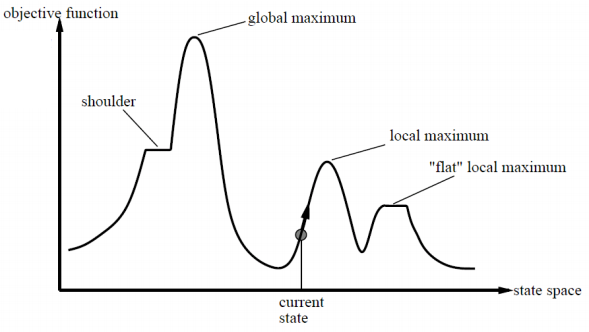
\includegraphics[scale=1]{statesspace.png}
\end{center}
Uno \textbf{stato ha una posizione sulla superficie} e un'\textbf{altezza corrispondente al valore della sua funzione di valutazione}. Un \textbf{algoritmo provoca un movimento sulla superficie}.\\
Trovare \textbf{avvallamento più basso} (es: costo minimo) \textbf{o il picco più alto} (es: massimo di un obiettivo)
\subsection{Algoritmo Hill Climbing}
Anche detto \textbf{ricerca in salita}, \textbf{steepest ascent/descent}.\\
Ricerca locale \textbf{greedy}.\\
Vengono generati i successori e valutati. Viene scelto un nodo che migliora la valutazione dello stato attuale (\textbf{non si tiene traccia degli altri}, quindi non ho l'albero di ricerca in memoria). La scelta del nodo dipende dall'algoritmo:
\begin{list}{}{}
	\item Migliore $\rightarrow$ \textbf{Hill Climbing a salita ripida}
	\item Uno a caso tra quelli che migliorano $\rightarrow$ \textbf{Hill Climbing Stocastico}
	\item Il primo $\rightarrow$ \textbf{Hill Climbing con prima scelta}
\end{list}
Se non ci sono stati migliori, l'algoritmo termina con \textbf{fallimento}.
\begin{lstlisting}
function Hill-climbing(problema) returns stato-massimo-locale
  nodo-corrente = CreaNodo(problema.Stato-iniziale)
  loop do
    vicino = successore di nodo-corrente di valore piu alto
    if (vicino.Valore <= nodo-corrente.Valore)
      return nodo-corrente.Stato #interrompe la ricerca
    nodo-corrente = vicino #altrimenti, se vicino migliore, continua
\end{lstlisting}
Si prosegue solo se il vicino più alto è migliore dello stato corrente, se tutti i vicini sono peggiori, si ferma. Non c'è frontiera a cui tornare, si tiene solo uno stato.\\
Tempo: numero di cicli variabile in base al punto di partenza.
\pagebreak
\paragraph{Problema delle 8 Regine} Con formulazione a stato completo
\begin{multicols}{2}
\begin{list}{}{}
	\item Costo $h$ $=$ numero di coppie di regine che si attaccano a vicenda
	\item I numeri sono i valori dei successori (7 $\times$ 8, 7 posizioni per ogni regina = su ogni colonna)
	\item Tra i migliori (valore 12) si \textbf{sceglie a caso}
	\item Minimo globale = 0
\end{list}
\begin{center}
	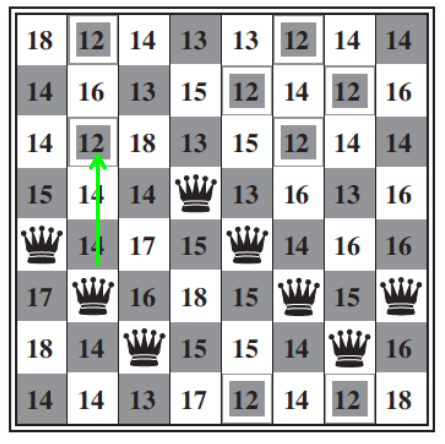
\includegraphics[scale=0.6]{8regstatcomp.png}
\end{center}
\end{multicols}
\begin{multicols}{2}
\begin{center}
	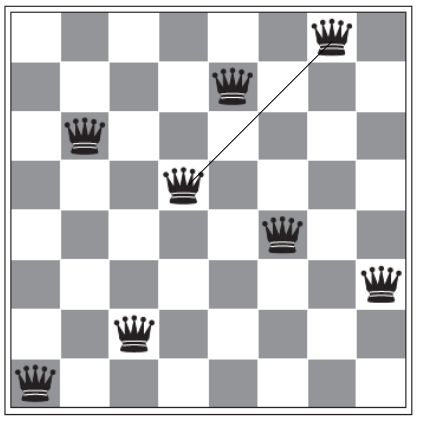
\includegraphics[scale=0.6]{8regstatcomp2.png}
\end{center}
\begin{list}{}{\textbf{Un minimo locale}}
		\item $h$ = 1
		\item Tutti gli stati successori non migliorano la situazione (minimo locale)
		\item \textbf{Per le 8 regine Hill-Climbing si blocca l'86\% delle volte}\\
		Ma in media sono 4 passi per la soluzione, e 3 quando si blocca
		\item Su $8^8$ = 17 milioni di stati
\end{list}
\end{multicols}
\paragraph{Esempio} Successo in tre mosse\\
$h$ qui è l'\textbf{euristica di costo della funzione obiettivo} da minimizzare
\begin{center}
	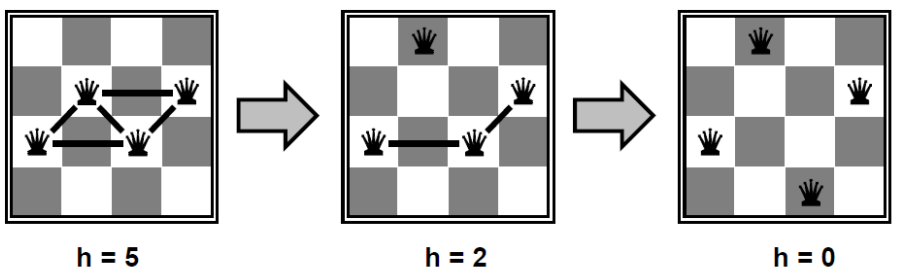
\includegraphics[scale=0.75]{8regine3passi.png}
\end{center}
\pagebreak
\subsubsection{Problemi con Hill-Climbing}
Se la funzione è da ottimizzare, i picchi sono massimi locali o soluzioni ottimali. Nel grafico si possono presentare: \textbf{massimi locali}, \textbf{plateu} (pianori), \textbf{spalle} e \textbf{crinali}/creste.
\paragraph{Miglioramenti}
\begin{enumerate}
	\item Consentire un \textbf{numero limitato di mosse laterali}\\
	Ossia ci si ferma per $<$ nell'algoritmo, anziché per $\leq$\\
	$\Rightarrow$ L'algoritmo sulle 8 regine ha successo nel 94\% dei casi, ma impiega in media 21 passi
	\item Hill-Climbing Stocastico: si \textbf{sceglie a caso tra le mosse in salita}, magari tenendo conto della pendenza.\\
	Converge più lentamente ma a volte trova soluzioni migliori
	\item Hill-Climbing con prima scelta: può generare le mosse a caso fino a trovarne una migliore dello stato corrente. Più \textbf{efficace quando i successori sono molti} (es: migliaia)
	\item Hill-Climbing con riavvio casuale (\textbf{random restart}): ripartire da un punto scelto a caso.\\
	Se la probabilità di successo è $p$, saranno necessarie in media $\frac{1}{p}$ ripartenze per trovare la soluzione (Es.: 8 regine, $p$ = 0.14, 7 iterazioni cioè 6 fallimenti e un successo).\\
	\textbf{Tendenzialmente completo}: insistendo si generano tutte le possibilità.\\
	Per le regine, 3 milioni di regine in meno di un minuto. Se funziona o no dipende molto dalla forma del panorama degli stati.
\end{enumerate}
\subsection{Algoritmo di Tempra Simulata}
\paragraph{Simulated Annealing} L'algoritmo di tempra simulata combina Hill-Climbing con una scelta stocastica ma \textbf{non del tutto casuale perché poco efficiente}. L'analogia è col processo di tempra dei metalli: portati a temperature molto elevate e raffreddati gradualmente consentendo di cristallizzare in uno stato a più bassa energia.
\paragraph{Tempra Simulata} Ad ogni passo si \textbf{sceglie un successore a caso}:
\begin{list}{}{}
	\item Se migliora lo stato corrente, viene espanso
	\item Se non lo migliora (caso in cui $\Delta E = f(n') - f(n) < 0$), quel nodo viene scelto con probabilità $p = e^{\Delta E/T}$, con $p$ ovviamente $0 \leq p \leq 1$\\
	(Si genera un numero casuale tra 0 e 1, se questo è $<$ $p$ il successore viene scelto, altrimenti no)
	\item $p$ è \textbf{inversamente proporzionale al peggioramento}
	\item $T$ (\textbf{temperatura}) \textbf{decresce al progredire dell'algoritmo}, quindi anche $p$, \textbf{secondo un piano definito}.\\
	Col progredire, rende improbabili le mosse peggiorative.
\end{list}
\paragraph{Analisi} La probabilità di una mossa in discesa diminuisce col tempo, e l'algoritmo si comporta sempre di più come Hill-Climbing.\\
Se $T$ viene decrementato abbastanza lentamente, con probabilità tendente ad 1 si raggiunge la soluzione ottimale.\\
\textbf{Analogia}: $T$ corrisponde alla temperatura e $\Delta E$ alla variazione di energia
\paragraph{Parametri} \textbf{Valore iniziale} e \textbf{decremento di $T$} sono parametri.\\
I valori per $T$ sono \textbf{determinati sperimentalmente}: il \textbf{valore iniziale di $T$} è \textbf{tale che per valori medi di $\Delta E$}, $p = e^{\Delta E/T}$ sia circa 0.5
\subsection{Algoritmo Local Beam}
Versione locale della beam search.\\
Si tengono in memoria $k$ stati invece che uno solo. Ad ogni passo si generano i successori di tutti i $k$ stati.
\begin{list}{}{}
	\item Se si trova un goal, ci si ferma
	\item Altrimenti si prosegue con i $k$ migliori tra questi
\end{list}
Note:
\begin{list}{}{}
	\item Diverso da K restart (che riparte da 0)
	\item Diverso da beam search
\end{list}
\pagebreak
\subsection{Algoritmo Beam Search Stocastico}
Si introduce un elemento di casualità, come in un processo di selezione naturale: \textbf{diversificare la nuova generazione}.\\
In questa variante stocastica, si scelgono $k$ successori ma \textbf{con probabilità maggiore per i migliori}. \textbf{Terminologia}:
\begin{list}{}{}
	\item \textbf{Organismo}, stato
	\item \textbf{Progenie}, successori
	\item \textbf{Fitness} (valore della $f$), idoneità
\end{list}
\section{Algoritmi Genetici}
\paragraph{L'Idea} Sono \textbf{varianti della beam search stocastica} in cui gli \textbf{stati successori sono ottenuti \textit{combinando} due stati genitore} anziché per evoluzione. \textbf{Terminologia}:
\begin{list}{}{}
	\item \textbf{Popolazione} di \textbf{individui} (stati)
	\item \textbf{Fitness}
	\item \textbf{Accoppiamenti} e \textbf{mutazione genetica}
	\item \textbf{Generazioni}
\end{list}
\paragraph{Funzionamento} \textbf{Popolazione iniziale}: $k$ stati/\textbf{individui} generati casualmente. Ogni \textbf{individuo è rappresentato come una stringa}: ad esempio 24 bit, o posizione nelle colonne ("\textit{24748552}") per le 8 regine.\\
Gli \textbf{individui} sono \textbf{valutati da una funzione di fitness}: ad esempio numero di coppie di regine che \textit{non} si toccano.\\
Si \textbf{selezionano gli individui per gli accoppiamenti}, con una probabilità proporzionale alla fitness. Le \textbf{coppie danno vita alla generazione successiva}: combinando materiale genetico (\textbf{crossover}) o con un meccanismo aggiuntivo di \textbf{mutazione genetica} (\textbf{casuale}).\\
La popolazione ottenuta dovrebbe essere migliore e la cosa si \textbf{ripete fino ad ottenere stati abbastanza buoni} (\textbf{stati obiettivo}).
\paragraph{Esempio}
\begin{center}
	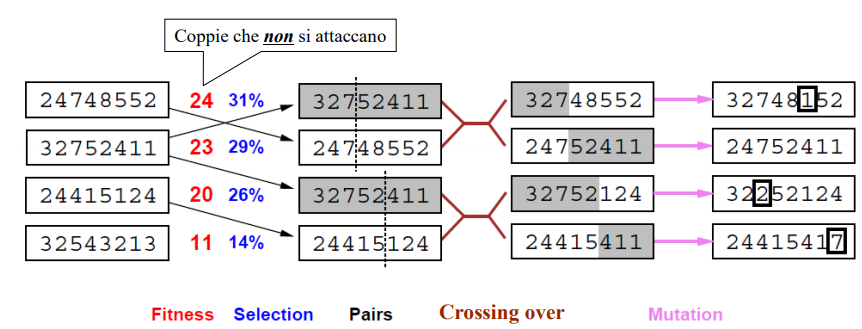
\includegraphics[scale=0.7]{alggenetic.png}
\end{center}
Per ogni coppia viene scelto un punto di \textbf{crossing over} (la linea tratteggiata) e vengono \textbf{generati due figli scambiandosi dei pezzi} \textit{del DNA}.\\
Viene infine effettuata una mutazione casuale che dà luogo alla prossima generazione.
\pagebreak
\paragraph{Nascita di un figlio}
\begin{center}
	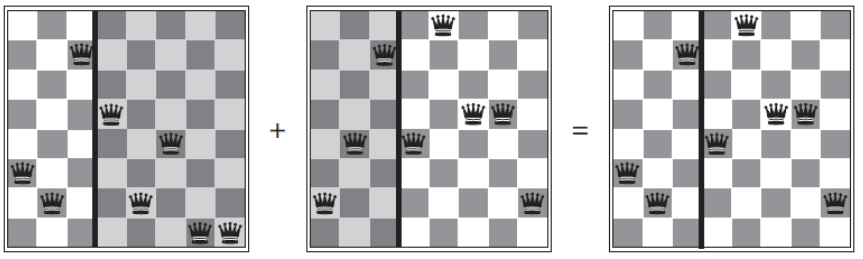
\includegraphics[scale=0.7]{8reggeneticfigli.png}
\end{center}
Le parti chiare sono passate al figlio, le parti scure si perdono. Se i genitori sono molto diversi, anche i nuovi stati sono diversi. All'inizio spostamenti maggiori che poi si raffinano.
\subsection*{Algoritmi Genetici}
\paragraph{Suggestivi} Area del \textbf{Natural Computing}. Usati molto in problemi reali (es.: configurazione di circuiti e scheduling dei lavori).\\
Combinano la tendenza a salire della beam search stocastica con l'interscambio di informazioni tra thread paralleli di ricerca (blocchi utili che si combinano).\\
Funziona meglio de il problema (soluzioni) ha componenti significative rappresentate in sottostringhe.\\
\textbf{Punto critico}: rappresentazione del problema in stringhe.
\paragraph{Spazi Continui} Molti casi reali hanno spazi di ricerca continua, fondamentale per il Machine Learning! Lo stato è descritto da variabili continue $x_1$, \ldots, $x_n$ (vettore $x$), ad esempio la posizione in uno spazio 3D $x = (x_1, x_2, x_3)$.\\
Apparentemente è complicato: fattori di ramificazione infiniti con gli approcci precedenti. Ma in realtà ci sono molti strumenti matematici per spazi continui, che portano ad approcci anche molto efficienti.
\subsection{Gradient}
Se la $f$ è \textbf{continua} e \textbf{differenziabile}, ad esempio quadratica rispetto il vettore $x$, allora il minimo/massimo lo si può cercare utilizzando il \textbf{gradiente}, che \textbf{restituisce la direzione di massima pendenza del punto}.\\
Data $f$ obiettivo $$\nabla f = \left( \frac{\partial f}{\partial x_1}, \frac{\partial f}{\partial x_2}, \frac{\partial f}{\partial x_3} \right)$$
\textbf{Hill-Climbing iterativo}: $x_{new} = x_{old} + \eta\nabla f(x)$ con $\eta$ dimensione dello step.\\
Quantifica lo spostamento, senza cercarlo tra gli infiniti possibili successori.\\
\textbf{Nota}: in generale non è sempre necessario il min/max assoluto. Vedremo nel ML.
\begin{center}
	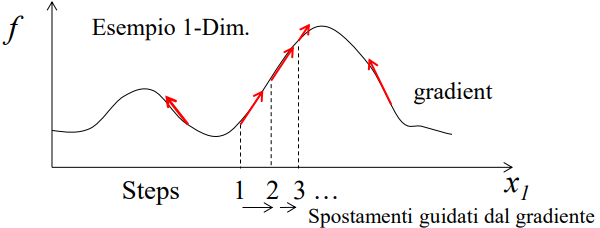
\includegraphics[scale=1]{gradient.png}
\end{center}
\pagebreak
\section{Ambienti più realistici}
\paragraph{Problemi classici} Gli agenti risolutori di problemi "classici" assumono:
\begin{list}{}{}
	\item Ambienti \textbf{completamente osservabili}
	\item Azioni e ambienti \textbf{deterministici}
	\item Piano generato è sequenza di azioni \textbf{eseguibile ad occhi chiusi}, generato \textit{offline} ed eseguito senza imprevisti
	\item Le \textbf{percezioni non servono}, se non nello stato iniziale
\end{list}
\paragraph{Soluzioni più complesse} In un ambiente \textbf{parzialmente osservabile} e \textbf{non deterministico} le \textbf{percezioni sono importanti}: \textbf{restringono gli stati} possibili e \textbf{informano} sull'effetto dell'\textbf{azione}.\\
Più che un piano, l'\textbf{agente elabora una strategia} che \textbf{tiene conto delle diverse eventualità}: un \textbf{piano con contingenza}. Esempio: aspirapolvere con assunzioni diverse.
\subsection{Azioni non deterministiche}
\paragraph{Aspirapolvere imprevedibile} Ci sono più stati possibili come risultato dell'azione.\\
\textbf{Comportamento}: se aspira in una stanza sporca la pulisce\ldots ma \textbf{a volte} pulisce anche una stanza adiacente. Se aspira in una stanza pulita, \textbf{a volte} rilascia sporco.
\paragraph{Variazioni necessarie al modello} Il modello di transizione, quindi, \textbf{restituisce un insieme di stati}: l'agente non sa in quale si troverà. Il \textbf{piano di contingenza} sarà un piano condizionale e magari con cicli.
\paragraph{Esempio}
\begin{multicols}{2}
Nell'esempio\\\texttt{Risultati(Aspira, 1) = \{5, 7\}}, cioè aspirando nello stato \texttt{1} posso finire nello stato \texttt{5} o \texttt{7}.\\
Un possibile piano è
\begin{lstlisting}
[Aspira,
	if (stato = 5):
		[Destra, Aspira]
	else:
		[]
]
\end{lstlisting}
Da sequenza di azioni a piano (albero)
\begin{center}
	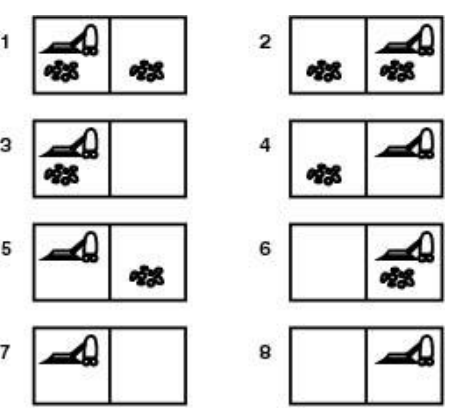
\includegraphics[scale=0.7]{aspirapolvereimprevedibile.png}
\end{center}
\end{multicols}
\subsection{Come si pianifica}
\paragraph{Alberi di Ricerca \texttt{AND-OR}}
\begin{list}{}{}
	\item Nodi \texttt{OR}: scelte dell'agente (1 sola azione)
	\item Nodi \texttt{AND}: le diverse contingenze (scelte dell'ambiente, più stati possibili), \textbf{da considerare tutte}
\end{list}
Una \textbf{soluzione ad un problema di ricerca \texttt{AND-OR}} è un \textbf{albero} che
\begin{list}{}{}
	\item Ha un nodo obiettivo in ogni foglia
	\item Specifica un'unica azione nei nodi \texttt{OR}
	\item Include tutti gli archi uscenti da nodi \texttt{AND}
\end{list}
\pagebreak
\paragraph{Esempio}
\begin{center}
	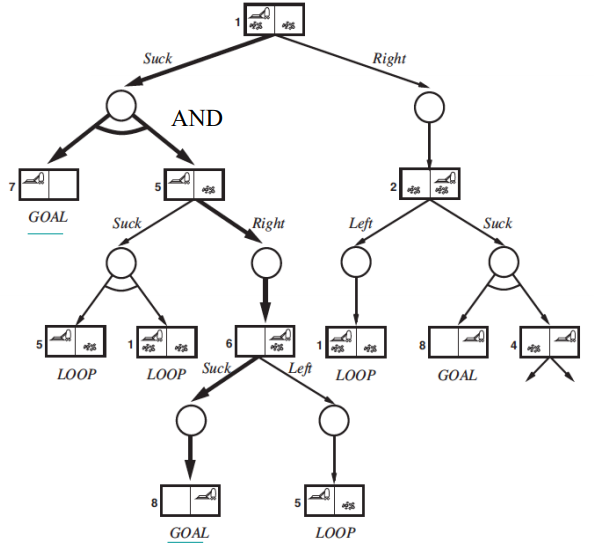
\includegraphics[scale=0.7]{andortree.png}
\end{center}
\textbf{Archi in grassetto} = soluzione (sottoalbero), la seguente:
\begin{lstlisting}
	Piano: [Aspira: if (stato = 5): [Destra, Aspira] else: []]
\end{lstlisting}
%https://elearning.di.unipi.it/pluginfile.php/30593/mod_resource/content/0/5-2020-oltre_ricerca_classica.pdf, p.38-78 saltate
\chapter{I Giochi con Avversario}
\paragraph{Premessa}
Fin'ora abbiamo avuto \textit{Problemi Solving} come ricerca. Il paradigma di base era: ambiente osservabile, deterministico, utente singolo e stati atomici.\\
Da adesso considereremo un \textbf{rilassamento delle assunzioni di base}: ambiente multi agente e rappresentazioni degli stati più complesse.\\
Ci occuperemo di \textbf{specializzazioni} del paradigma nell'ambito dei giochi con avversario: quindi i piani d'azione devono tenere conto dell'avversario.\\
Vedremo \textbf{problemi di soddisfacimento di vincoli}, sempre come ricerca in spazio di soluzioni, con stato a struttura \textbf{fattorizzata}.\\\\
Questo ci porterà a considerare \textbf{sistemi basati su conoscenza}: lo stato è una "\textbf{base di conoscenza}" a cui rivolgere domande, con una rappresentazione in un linguaggio espressivo e \textbf{tecniche di "ragionamento" con inferenze}: logica del prim'ordine e calcolo proposizionale.
\section{Giochi con Avversario}
\begin{list}{-}{}
	\item Regole semplici e formalizzabili
	\item Ambiente accessibile e deterministico
	\item Due giocatori, a turni alterni, a \textbf{somma zero} (se uno vince, l'altro perde: sommare i punteggi dà 0 o comunque un risultato costante), a informazione perfetta (tutti i giocatori conoscono lo stato attuale del gioco)
	\item Ambiente multi-agente competitivo: la presenza dell'avversario rende l'\textbf{ambiente strategico}, più difficile rispetto a quanto visto fin'ora
	\item Complessità e vincoli di tempo reale: mossa migliore nel tempo disponibile
\end{list}
$\Rightarrow$ Questa tipologia di giochi sono un po' più simili ai problemi reali
\subsection{Ciclo \textit{pianifica-agisci-percepisci}}
\paragraph{Due agenti a turno} Si può pianificare considerando le possibili risposte dell'avversario e le possibili risposte a quelle risposte\ldots e così via.\\
Una volta decisa la mossa
\begin{list}{}{}
	\item Si \textbf{esegue} la mossa
	\item Si \textbf{vede} cosa fa l'avversario
	\item Si \textbf{pianifica} la prossima mossa
\end{list}
\pagebreak
\section{Giochi come problemi di ricerca}
\begin{list}{}{}
	\item \textbf{Stati}: configurazioni del gioco
	\item \textbf{Player(s)}: a chi tocca muovere nello stato \textbf{s}
	\item \textbf{Stato iniziale}: configurazione iniziale gioco
	\item \textbf{Actions(s)}: mosse legali in \textbf{s}
	\item \textbf{Result(s, a)}: stato risultante da una mossa
	\item \textbf{Terminal-Test(s)}: determina se stato è fine del gioco
	\item \textbf{Utility(s, p)}: utilità (o \textbf{pay-off}), cioè valore numerico degli stati terminali del gioco per il giocatore \textbf{p}\\
	Es: 1, -1, 0, conteggio punti\ldots
\end{list}
\subsection{Algoritmo MinMax}
Valuto gli stati terminali in base al punteggio/vittoria che ottengo, poi valuto gli stati preterminali in base allo stato terminale in cui mi portano (se mi portano a vittoria o meno a ritroso).\\
Valuto gli stati intermedi con il valore \textbf{min}imo dei risultati se tocca all'avversario (minimo rischio) e col valore \textbf{ma}ssimo se tocca a me.
\begin{center}
	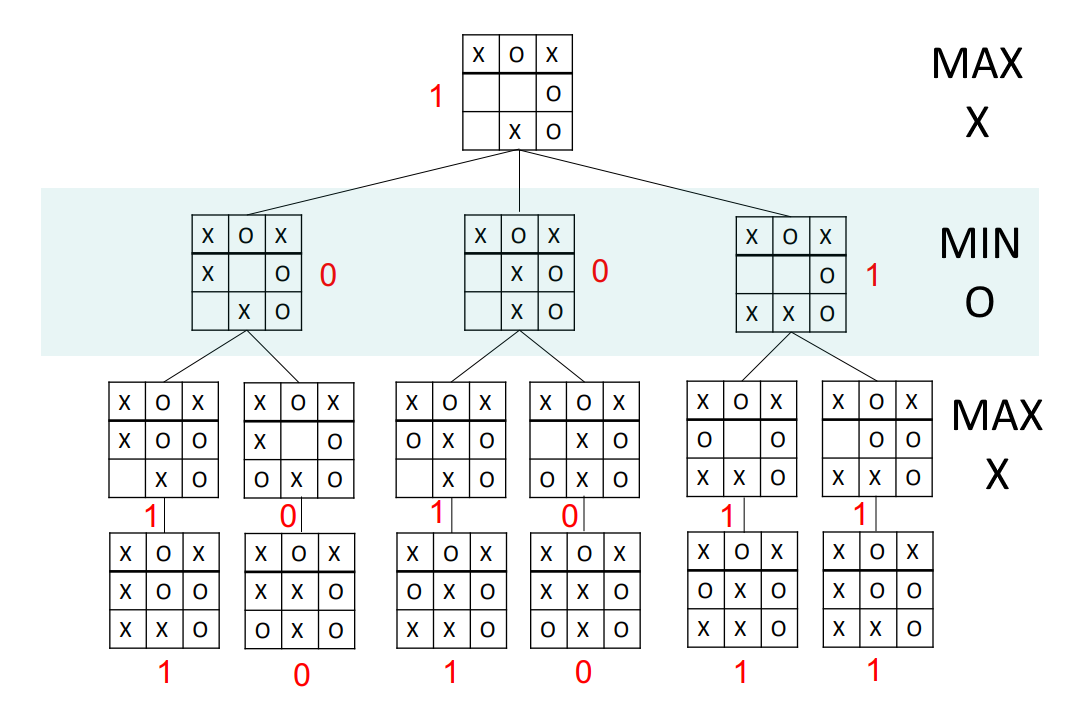
\includegraphics[scale=0.45]{minmax_tictactoe.png}
\end{center}
\paragraph{Valore MinMax} \textbf{Minimax(s)} = 
\begin{math}
\left\{
\begin{array}{c c}
	\textbf{Utility(s, Max)} & \textsl{se}\:\:\textbf{Terminal-Test(s)}\\
	max_{a \in Action(s)} \textbf{Minimax(Result(s, a))} & \textsl{se}\:\: \textbf{Player(s) = MAX}\\
	min_{a \in Action(s)} \textbf{Minimax(Result(s, a))} & \textsl{se}\:\: \textbf{Player(s) = min}
\end{array}
\right.
\end{math}
\paragraph{Come conviene esplorare l'albero di gioco?} In profondità, perché hanno ampiezza esponenziale.
\pagebreak

\paragraph{Algoritmo ricorsivo} Di seguito
\begin{center}
	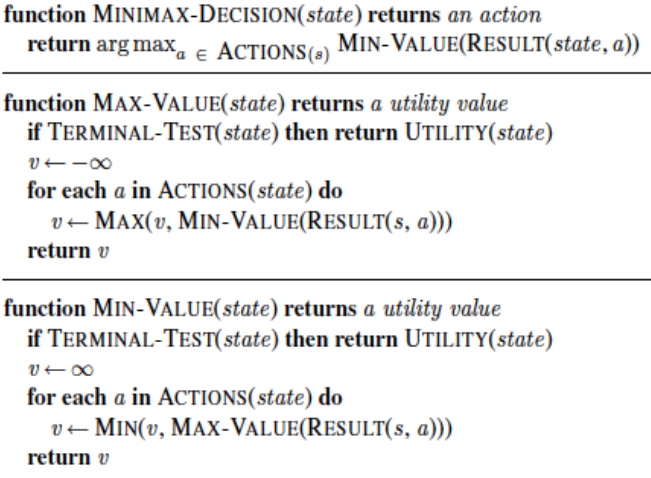
\includegraphics[scale=0.7]{minimaxricorsivo.png}
\end{center}
\begin{center}
	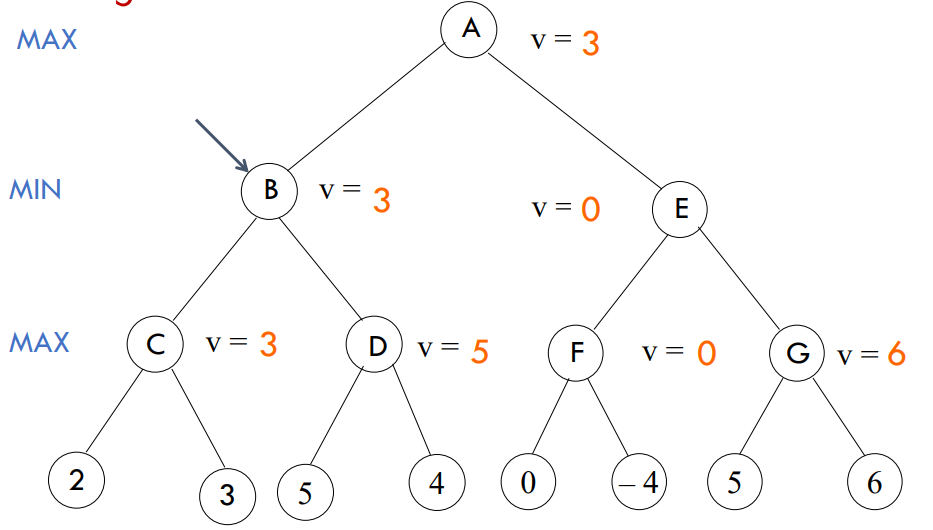
\includegraphics[scale=0.7]{minimaxes.png}
\end{center}
\paragraph{Costo}
\begin{list}{}{}
	\item Tempo: come DF $\rightarrow$ O(b$^m$)
	\item Spazio: O(m)
	\item Per gli scacchi ($10^{40}$ nodi) più di $10^{22}$ secoli $\Rightarrow$ improponibile un'esplorazione sistematica del grafo, se non per giochi molto semplici
	\item Necessarie \textbf{euristiche}
\end{list}
\pagebreak
\subsection{Algoritmo Min-Max Euristico (con orizzonte)}
In casi più complessi, dove esplorare stati è troppo costoso (es. scacchi), occorre una \textbf{funzione di valutazione euristica}.
\paragraph{Strategia} Guardare avanti $d$ livelli
\begin{list}{}{}
	\item Si espande l'albero di ricerca un certo numero di livelli $d$, compatibile con il tempo e lo spazio disponibili
	\item Si \textbf{valutano gli stati ottenuti} e si propaga indietro il risultato con la regola del Minimax
\end{list}
L'algoritmo è simile a prima ma\\
\texttt{if Terminal-Test(s) then return Utility(s)} $\rightarrow$ \texttt{if Cutoff-Test(s, d) then return Eval(s)}\\\\
Posto $d$ limite della profondità consentita\\
\textbf{H-Minimax(s, d)} = 
\begin{math}
\left\{
\begin{array}{c c}
	\textbf{Eval(s)} & \textsl{se}\:\:\textbf{Cutoff-Test(s, d)}\\
	max_{a \in Action(s)} \textbf{H-Minimax(Result(s, a), d + 1)} & \textsl{se}\:\: \textbf{Player(s) = MAX}\\
	min_{a \in Action(s)} \textbf{H-Minimax(Result(s, a), d + 1)} & \textsl{se}\:\: \textbf{Player(s) = min}
\end{array}
\right.
\end{math}
\begin{center}
	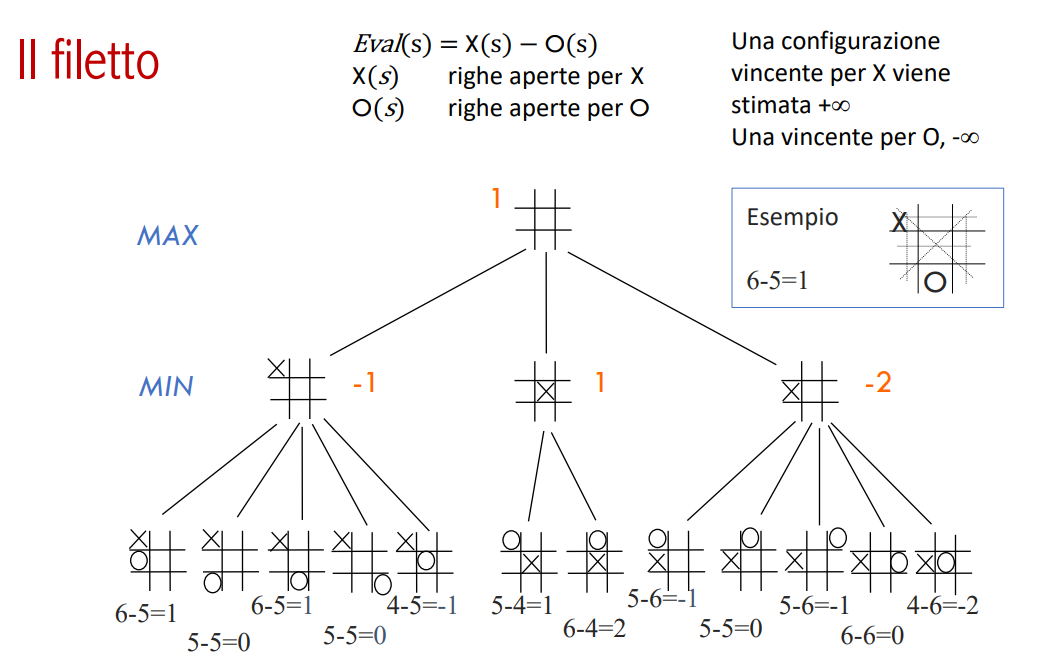
\includegraphics[scale=0.5]{hminmax_tictactoe.png}
\end{center}
\subsubsection{Funzione di Valutazione}
La funzione di valutazione \textbf{Eval} è una \textbf{stima dell'utilità attesa} a partire da una certa posizione. La qualità della \textbf{funzione} è determinante.
\begin{list}{}{}
	\item deve essere \textbf{consistente} con l'utilità se applicata agli stati terminali del gioco (indurre lo stesso ordinamento)
	\item deve essere \textbf{efficiente} da calcolare
	\item deve \textbf{riflettere} le probabilità effettive di vittoria (A valutato meglio di B se da A ho più probabilità di vittoria rispetto a B)
	\item combina probabilità con utilità dello stato terminale, può essere appreso con l'esperienza
\end{list}
\paragraph{Esempio} \textbf{Scacchi}\\
Si potrebbe pensare di valutare caratteristiche diverse dello stato: valore del materiale (pedone 1, cavallo/alfiere 3, torre 5, regina 9\ldots), buona disposizione dei pedoni, protezione del re\ldots\\
Funzione lineare pensata $Eval(s) = w_1f_1(s) + w_2f_2(s) + \ldots + w_nf_n(s)$\\
Ma anche combinazioni non lineari delle caratteristiche: alfiere vale di più a fine partita, due alfieri valgono più del doppio di uno solo\ldots
\pagebreak
\paragraph{Problemi Noti}
\begin{list}{}{}
	\item \textbf{Stati Non Quiescienti}: l'esplorazione fino ad un certo livello può mostrare una situazione molto vantaggiosa, ma la mossa successiva risulta estremamente svantaggiosa es. regina mangiata dalla torre. Si possono riconoscere.\\
	\textbf{Soluzione}: \textbf{non fermarsi agli stati non quiescienti} ma esplorare un po' di più fino ad arrivare a stati in cui la funzione di valutazione non attende variazioni repentine (\textbf{stati quiescienti})
	\item \textbf{Effetto Orizzonte}: si privilegiano \textbf{mosse diversive che hanno solo l'effetto di spingere il problema oltre}, per evitare mosse disastrose che alla fine devono per forza accadere
\end{list}
\paragraph{Ottimizzazione} Dobbiamo esplorare ogni cammino? No, \textbf{esistono tecniche di potatura} che dimezzano la ricerca pur mantenendo decisione min-max corretta (\textbf{potatura alfa-beta})
\paragraph{Potatura Alfa-Beta} ridurre spazi ricerca algoritmi min-max
\subsection{Potatura Alfa-Beta}
Tecnica di \textit{potatura} per ridurre l'esplorazione dello spazio di ricerca in algoritmi minmax
\paragraph{Idea}
\begin{center}
	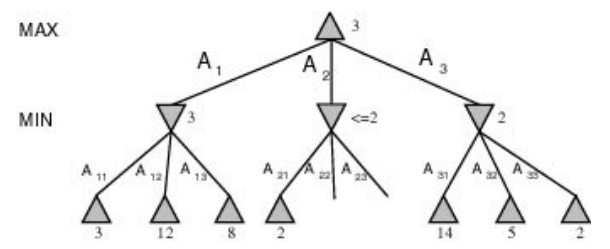
\includegraphics[scale=0.7]{minmaxidea.png}
	$$minmax(radice) = max(min(3, 12, 8), min(2, x, y), min (14, 5, 2)) =$$ $$= max(3, min(2, x, y), 2) =$$ $$= max(3, z, 2) = 3)\:\:\:\:\:\:\textsl{con}\:z \leq 2$$
\end{center}
\paragraph{Algoritmo} Consideriamo un nodo $v$: se c'è una \textbf{scelta migliore sopra}, allora quel $v$ non sarà mai raggiunto.\\
Max passerà da $\alpha$ piuttosto che finire a $v$.
\paragraph{Implementazione} Si va avanti in profondità fino al livello desiderato e, propagando indietro i valori, si decide se si può abbandonare l'esplorazione nel sotto-albero.
\begin{list}{}{}
	\item \textbf{MaxValue} e \textbf{MinValue} vengono invocate con \textbf{due valori di riferimento iniziali}\\
	$MaxValue = \alpha$ (inizialmente $-\infty$)\\
	$MinValue = \beta$ (inizialmente $+\infty$)
	\item Rappresentano \textbf{rispettivamente} la \textbf{migliore alternativa per Max e per Min} fino a quel momento
	\item \textbf{I tagli avvengono quando}, nel propagare indietro, si verifica:\\
	$v \geq \beta$ per i nodi Max (taglio $\beta$)\\
	$v \leq \alpha$ per i nodi Min (taglio $\alpha$)
\end{list}
\pagebreak
\begin{center}
	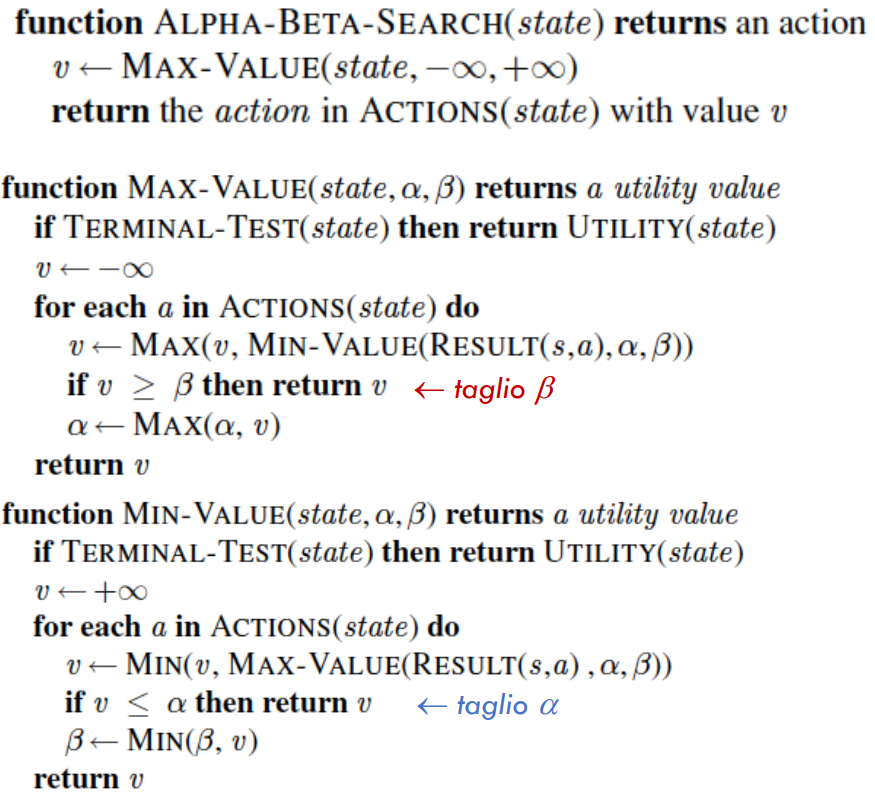
\includegraphics[scale=0.5]{alphabetalag.png}
\end{center}
\paragraph{Ordinamento delle mosse} La \textbf{potatura ottimale} si ottiene quando ad ogni livello sono generate prima le mosse migliori per chi gioca:
\begin{list}{}{}
	\item Per i \textbf{nodi Max} sono generate prima le mosse con valore più \textbf{alto}
	\item Per i \textbf{nodi Min} sono generate prima le mosse con valore più \textbf{basso}
\end{list}
\paragraph{Complessità} O(b$^{m/2}$)\\
Alfa-Beta \textbf{può arrivare a profondità doppia rispetto a MinMax}, ma come avvicinarsi all'ordinamento ottimale?
\paragraph{Ordinamento Dinamico} Usando un approfondimento iterativo si possono \textbf{scoprire ad una iterazione delle informazioni utili per l'ordinamento delle mosse}, da usare in una successiva iterazione (\textbf{mosse killer}).\\
\textbf{Tabella delle trasposizioni}: per ogni stato incontrato si memorizza la sua valutazione: situazione tipica è quando $[a_1, b_1, a_2, b_2]$ e $[a_1, b_2, a_2, b_1]$ portano nello stesso stato.
\paragraph{Altri miglioramenti}\begin{list}{}{}
	\item \textbf{Potatura in avanti} Esplorare solo \textbf{alcune mosse ritenute promettenti} e tagliare le altre: beam search, tagli probabilistici basati su esperienza
	\item \textbf{Database di mosse} di apertura e chiusura: nelle prime fasi ci sono poche mosse sensate e ben studiate, mentre per le fasi finali il computer può esplorare in maniera esaustiva e ricordarsi le chiusure migliori
\end{list}
\paragraph{Giochi Multiplayer} Invece di aver due valori ho un vettore di valori per nodo. Per propagare all'indietro prendo vettore che migliora la valutazione.
\paragraph{Giochi più complessi}
\begin{list}{}{}
	\item \textbf{Giochi stocastici}, con un lancio di dadi
	\item \textbf{Giochi parzialmente osservabili}: \textbf{deterministici} (mosse deterministiche ma non si conoscono gli effetti delle mosse dell'avversario, es: battaglia navale), \textbf{stocastici} (carte distribuite a caso come in molti giochi)
\end{list}
\pagebreak
\chapter{Problemi di Soddisfacimento di Vincoli}
\paragraph{CSP} Sono problemi con una struttura particolare, che si prestano ad algoritmi di ricerca specializzati. Grazie alla struttura si cerca meglio la soluzione: rappresentazione \textbf{fattorizzata}, con la quale iniziamo a dire qualcosa sulla struttura dello stato.
\paragraph{Classe ampia} Questa classe di problemi è molto ampia, esistono \textbf{euristiche generali} da applicare e che consentono la risoluzione di istanze con dimensioni significative.
\section{Formulazione} 
\begin{list}{}{}
	\item\textbf{Problema} descritto da \textbf{tre componenti}:
		\begin{list}{}{}
			\item \textbf{X}, insieme di \textbf{variabili}
			\item \textbf{D}, insieme di \textbf{domini}\\
			Dove D$_i$ è l'insieme dei valori possibili per X$_i$
			\item \textbf{C}, insieme di \textbf{vincoli}, relazioni tra le variabili
		\end{list}
	\item\textbf{Stato}, un \textbf{assegnamento parziale/completo} di valori a variabili\\
	\{X$_i$ = v$_i$, X$_j$ = v$_j$, \ldots\}\\
	\textbf{Stato iniziale}: \{\}
	\item \textbf{Azioni}: assegnamento di un valore ad una variabile, tra quelli leciti
	\item \textbf{Soluzione} (goal test): \textbf{assegnamento completo} (tutte le variabili hanno un valore) e \textbf{consistente} (i vincoli sono tutti soddisfatti)
\end{list}
\paragraph{Esempio} Il problema delle 8 regine
\begin{list}{}{}
	\item X = \{Q$_1$, \ldots, Q$_8$\}
	\item D$_i$ = \{1, 2, 3, 4, 5, 6, 7, 8\}
	\item C$_i$ i vincoli di non attacco\\
	Esempio di vincolo fra Q$_1$ e Q$_2$: $<$(Q$_1$, Q$_2$), \{(1, 3), (1, 4), (1, 5), (1, 6), (1, 7), (1, 8), (2, 5), \ldots\}$>$
	\item Formulazione incrementale o a stato completo
\end{list}
\section{Strategie per problemi CSP}
Fin'ora potevamo solo ricercare la soluzione nel grafo degli stati, guidati da una metrica definita sullo stato. Adesso possiamo:
\begin{list}{}{}
	\item Usare delle euristiche specifiche per questa classe di problemi
	\item Fare delle inferenze che ci portano a restringere i domini, quindi a \textbf{limitare la ricerca}: \textbf{propagazione di vincoli}
	\item Fare \textbf{backtracking intelligente}
\end{list}
Tipicamente \textbf{un misto di queste strategie}.
\pagebreak
\subsection{Ricerca in problemi CSP}
Ad ogni passo si assegna una variabile: la massima profondità della ricerca è fissata dal numero di variabili $n$.
\paragraph{Versione \textit{ingenua}} L'ampiezza dello spazio di ricerca è $|D_1| \times |D_2| \times \ldots \times |D_n|$, dove $|D_i|$ è la cardinalità del dominio di X$_i$.\\
Il fattore di diramazione è pari a $n\cdot d$ al primo passo, $(n-1)\cdot d$ al secondo\ldots le foglie sarebbero $n!\cdot d^n$\\
C'è una drastica riduzione dello spazio di ricerca, dovuta al fatto che il \textbf{Goal-Test} è \textbf{commutativo}: l'ordine con cui si assegnano le variabili non è importante). In realtà, quindi, il fattore di diramazione è pari alla dimensione dei domini $d$ ($d^n$ foglie).
\subsection{Backtracking}
\paragraph{BT} Ricerca con backtracking a profondità limitata: \textbf{controllo anticipato} della violazione dei vincoli. Intuile andare avanti fino alla fine e poi controllare, si può \textbf{fare backtracking non appena si scopre che un vincolo è stato violato}.\\
La ricerca è limitata naturalmente in profondità dal numero di variabili, quindi il metodo è completo.\\
\textbf{Scelta delle variabili} 
\begin{list}{}{}
	\item\textbf{MRV} (minimum remaining values): scegliere la \textbf{variabile con meno valori legali residui}, cioè \textbf{quella più vincolata}. Si scoprono prima i fallimenti (\textbf{fail first})
	\item\textbf{Euristica del grado}: scegliere la \textbf{variabile coinvolta in più vincoli} con le altre variabili (\textbf{quella più vincolante}, o di grado maggiore).\\
	Da usare a parità di MRV
\end{list}
\textbf{Scelta dei valori}: scegliere il \textbf{valore meno vincolante}, quello che esclude meno valori possibili per le altre variabili. Meglio valutare prima assegnamento che ha più probabilità di successo.\\
\textbf{Propagazione dei vincoli}
\begin{list}{}{}
	\item \textbf{Verifica in avanti}, Forward Checking: meno costosa, una volta assegnato il valore vado a vedere le variabili direttamente collegate nel grafo dei vincoli (non itero)
	\item \textbf{Consistenza di nodo e d'arco}: più costosa ma anche più efficace, restringono i valori dei domini delle variabili tenendo conto dei vincoli unari e binari su tutto il grafo (itero finché tutti nodi e archi sono consistenti)
\end{list}
\paragraph{Backtracking ricorsivo per CSP}
\begin{center}
	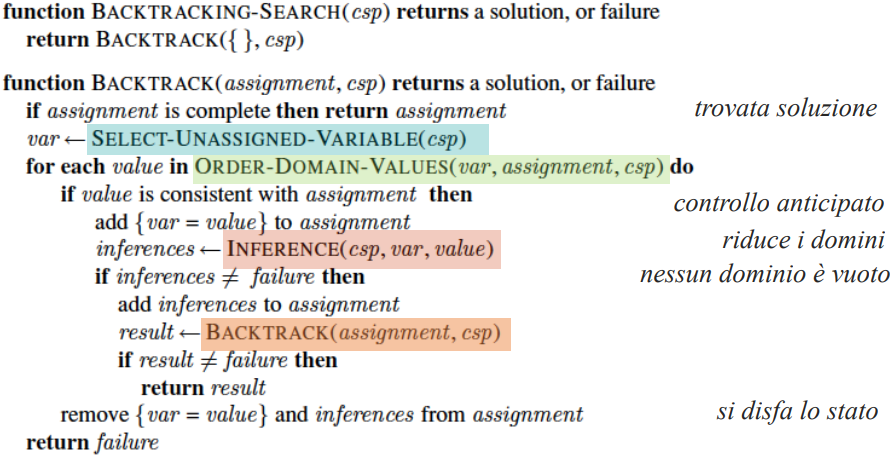
\includegraphics[scale=0.7]{cspbtricorsivo.png}
\end{center}
\paragraph{Esempio di FC} (Forward Check) Colorare mappa con Rosso, Verde, Blu.
\begin{center}
	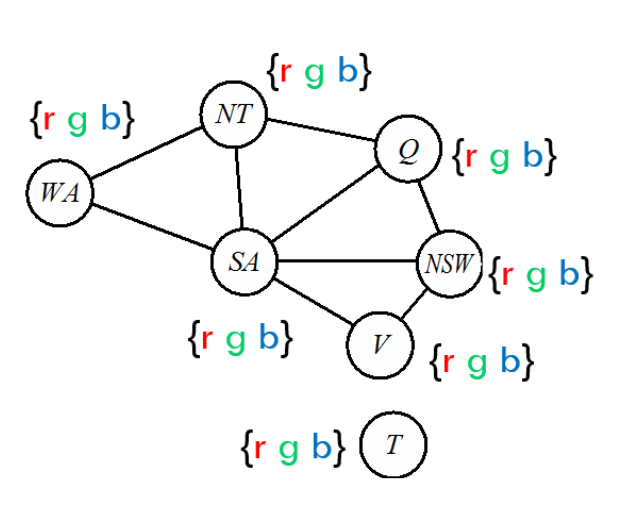
\includegraphics[scale=0.7]{FC_es1.png}
\end{center}
\paragraph{Backtracking Cronologico}
Suppongo di avere \{Q=R, NSW=G, V=B, T=R\} e cerco di assegnare SA. Il fallimento genera un backtracking cronologico: \textbf{si provano tutti i valori alternativi per l'ultima variabile}, T, continuando a fallire\ldots\\
Questo perché \textbf{non è la T responsabile del fallimento ma le altre variabili}.\\
Quindi si può fare un \textbf{backtracking "intelligente" guidato dalle dipendenze}.
%
\paragraph{Backtracking guidato dalle dipendenze} Considero le alternative solo per le variabili che hanno causato il fallimento \{Q, NSW, V\}, l'\textbf{insieme dei conflitti}.
\paragraph{Metodi CSP locali} I problemi CSP possono essere affrontati con metodi locali. Esempio: \textbf{le regine}.\\
\textbf{Euristica dei conflitti minimi} (\textbf{min-conflicts}): si sceglie un valore che crea meno conflitti. Solitamente si sceglie a caso una delle regie che violano dei vincoli.\\
Molto efficace: 1 milione di regine in 50 passi!
\begin{center}
	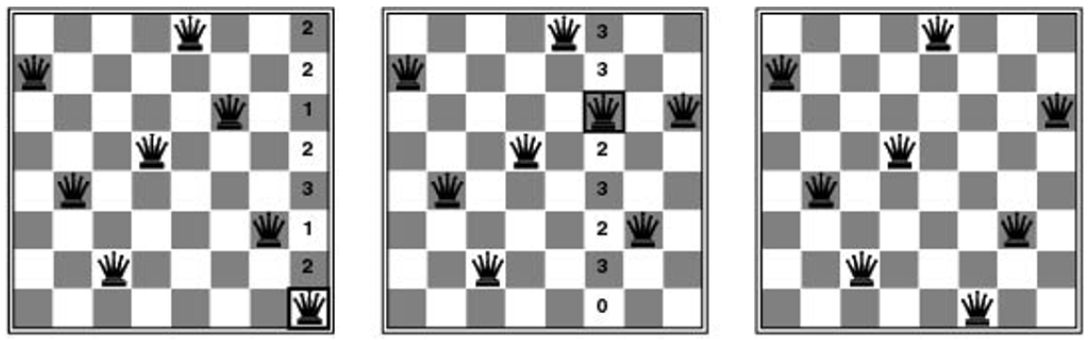
\includegraphics[scale=0.5]{minconflicts_es.png}
\end{center}
\paragraph{Conclusioni} Abbiamo visti due domini specifici per paradigma risoluzione problemi ricerca: giochi con avversario (complicazione: ambiente strategico e vincoli di tempo reale, non posso pianificiare azioni da eseguire "a occhi chiusi") e CSP (grazie a rappresenztazione stato più ricca tecniche problem solving specializzabili e usate per risolvere istanze di problemi di dimensioni maggori)\\
Prossimamente: \textbf{sistemi basati su conoscenza}. Conoscenza implica capacità inferenziali, con rappresentazione stato ancora più ricco con linguaggio rappresentazione conoscenza. L'inferenza è anch'essa un problema di ricerca in uno spazio di stati.
%TODO da qua
%https://elearning.di.unipi.it/pluginfile.php/30946/mod_resource/content/1/KRProp.pdf
\chapter{Agenti Basati su Conoscenza}
\paragraph{Fin'ora} Abbiamo trattato agenti con stato e con obiettivo, in mondi osservabili, con stati atomici e azioni descrivibili in maniera semplice, facendo \textbf{enfasi sul processo di ricerca}.\\
Poi abbiamo trattato descrizioni \textbf{fattorizzate}, come nel CSP, che consentono di iniziare a \textit{guardare dentro} lo stato, descritto come un \textbf{insieme di caratteristiche rilevanti} (\textbf{feature})
\paragraph{Adesso} Vedremo come costruire agenti dotati di capacità inferenziali. Cerchiamo di \textbf{migliorare la capacità di ragionamento}, dotando gli agenti di rappresentazioni del mondo più complesse non descrivibili semplicemente.\\
\textbf{Agenti basati su conoscenza}, con all'interno una \textbf{base di conoscenza} (\textbf{knowledge base}, o \textbf{KB}) con conoscenza espressa in forma esplicita e dichiarativa attraverso un \textbf{linguaggio}.
\section{Agenti Knowledge-Based}
\begin{center}
	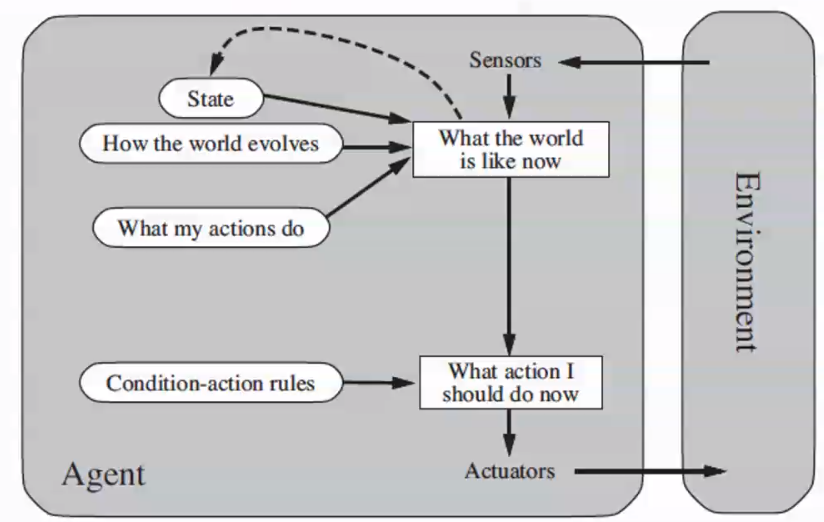
\includegraphics[scale=0.7]{ag_conosc.png}
\end{center}
La maggior parte dei problemi di I.A. sono "\textit{knowledge-intensive}". Il mondo è tipicamente \textbf{complesso}: serve una rappresentazione parziale e incompleta (\textbf{astrazione}) del mondo utile agli scopi dell'agente.\\
Per ambienti parzialmente osservabili e complessi ci servono linguaggi di rappresentazione della conoscenza più espressivi e \textbf{capacità inferenziali}.\\
La conoscenza può essere codificata a mano, acquisita o estratta da testi ed esperienza.
\pagebreak
\paragraph{Approccio dichiarativo vs procedurale}
Tipicamente la conoscenza in una KB viene espressa in \textbf{forma dichiarativa}. L'alternativa è \textbf{codificare la conoscenza in maniera procedurale}, attraverso un programma che implementa il processo decisionale. Un agente KB (con conoscenza dichiarativa) è più flessibile: perché è più semplice ricevere conoscenza in maniera incrementale e modificare il comportamento con l'esperienza.
\subsection{Il mondo del Wumpus}
\paragraph{Esempio} Agente in 1, 1: esplorare e trovare oro
\begin{multicols}{2}
\begin{list}{}{\textbf{Misura delle prestazioni}}
	\item \texttt{+1000} se trova l'oro, torna in \texttt{[1, 1]} ed esce
	\item \texttt{-1000} se muore
	\item \texttt{-1} per ogni azione
	\item \texttt{-10} se usa la freccia
\end{list}
\begin{list}{}{\textbf{Percezioni}}
	\item \textit{puzzo} nelle caselle adiacenti al Wumpus
	\item \textit{brezza} nelle caselle adiacenti alle buche
	\item \textit{luccichio} nelle caselle con l'oro
	\item \textit{bump} se batte in un muro
	\item \textit{urlo} se il Wumpus viene ucciso
	\item L'agente non percepisce la sua locazione
\end{list}
\begin{list}{}{\textbf{Azioni}}
	\item \textbf{Avanti}
	\item \textbf{A destra} di 90 gradi
	\item \textbf{A sinistra} di 90 gradi
	\item \textbf{Scaglia la freccia} (solo una)
	\item \textbf{Esce}
\end{list}
\columnbreak

Ambienti generati a caso, con \texttt{[1, 1]} \textit{safe}.
\begin{center}
	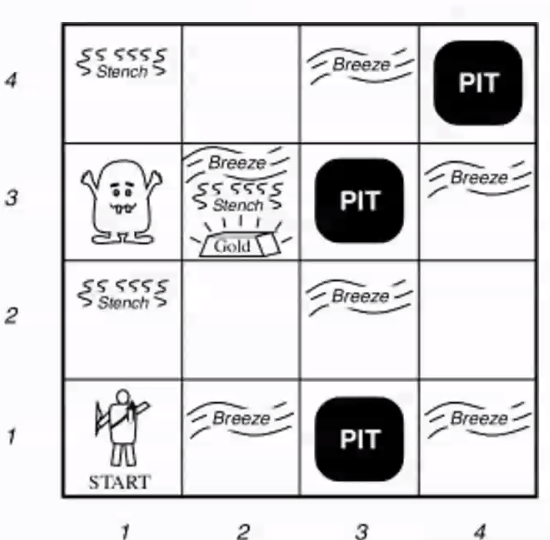
\includegraphics[scale=0.6]{wumpus.png}
\end{center}
\end{multicols}
\subsection{Knowledge-Base}
\paragraph{KB} Insieme di \textbf{enunciati} espressi in un linguaggio di rappresentazione.\\
L'agente interagisce con una KB con un'interfaccia funzionale \textbf{Tell-Ask}:
\begin{list}{}{}
	\item \textbf{Tell} per \textbf{aggiungere} nuovi enunciati alla KB
	\item \textbf{Ask} per \textbf{interrogare} la KB
	\item \textbf{Retract} per \textbf{eliminare} enunciati
\end{list}
\textbf{Enunciati} in KG \textbf{rappresentano la conoscenza} agente. Le \textbf{risposte $\alpha$} devono essere tali che $\alpha$ \textbf{è una conseguenza della KB}.
\paragraph{Problema} Il problema da risolvere: data una base di conoscenza KB che contiene una rappresentazione dei fatti ritenuti veri, vorrei sapere se un certo fatto $\alpha$ è vero di conseguenza, cioè vorrei sapere se 
\begin{center}
KB $\vDash \alpha$ $\:\:\:\:\-:\:\:\:\:\:$ (\textbf{conseguenza logica})
\end{center}
\pagebreak

\paragraph{Programma di un agente KB} Di seguito
\begin{lstlisting}
function Agente-KB (percezione) returns azione
	persistent:	KB, una base di conoscenza
			t, un contatore, inizialmente a 0, che indica il tempo
	TELL(KB, Costruisci-Formula-Percezione(percezione, t ))
	azione = ASK(KB, Costruisci-Query-Azione( t ))
	TELL(KB, Costruisci-Formula-Azione(azione, t ))
	t = t + 1
	return azione
\end{lstlisting}
\paragraph{KB vs DB} Una \textbf{base di conoscenza} è una \textbf{rappresentazione esplicita}, \textbf{parziale} e compatta in un linguaggio simbolico: contiene sia fatti espliciti (es. \textit{Pozzo in \texttt{[3, 3]}}) ma anche fatti generali o regole (es: brezza in caselle adiacenti a pozzi)\\
Una \textbf{base di dati} invece contiene solo fatti specifici e consente solo il recupero.\\
La differenza è che \textbf{la KB ha capacità inferenziale}: si possono \textbf{derivare nuovi fatti} da quelli memorizzati esplicitamente.
\paragraph{Trade-Off Fondamentale della Rappresentazione della Conoscenza} Trovare il \textbf{giusto compromesso tra l'espressibità} del linguaggio di rappresentazione \textbf{e la complessità} del meccanismo inferenziale.\\
Più un linguaggio è espressivo meno è efficiente il meccanismo inferenziale. Questi due obiettivi sono in contrasto, bisogna mediare e trovare un \textbf{compromesso}.\\
\subsubsection{Formalismi per la Rappresentazione della Conoscenza} Un formalismo per la rappresentazione della conoscenza ha tre componenti:
\begin{list}{}{}
	\item \textbf{Sintassi}: un linguaggio composto da un vocabolario e da regole per la formazione delle frasi (\textbf{enunciati})
	\item \textbf{Semantica}: stabilisce la corrispondenza tra gli enunciati e fatti del mondo. Se un agente ha un enunciato $\alpha$ nella sua KB, allora crederà che il fatto corrispondente ad $\alpha$ sia vero nel mondo
	\item \textbf{Meccanismo Inferenziale}: codificato o meno tramite regole di inferenza come nella logica, che ci consente di inferire nuovi fatti
\end{list}
\paragraph{Logica come linguaggio}
Qual è la complessità computazionale del problema KB $\vDash \alpha$ nei vari linguaggi logici? Quali algoritmi decisione e strategia ottimizzazione?\\
Linguaggi logici: calcolo proposizionale (POP) e logica dei predicati (FOL). Sono adatti per la rappresentazione della conoscenza? Da una parte sono anche troppo complessi, in particolare il FOL. Dall'altra, ci sono meccanismi non posseduti da FOL e POP ma che sono utili nelle KB.\\
Rivistazione di PROP e FOL per rappresentazione conoscenza, con attenzione ad algoritmi e complessità. \textbf{Contrazioni}: linguaggi a regole e \textbf{programmazione logica}.

\subsection{Algoritmo TT-entails}
KB $\vDash \alpha$?
\begin{list}{}{}
	\item Enumera tutte possibili interpretazioni KB ($k$ simboli, $2^k$ possibili interpretazioni)
	\item Per ciascuna interpretazione
	\begin{list}{}{}
		\item Se non soddisfa KB, OK
		\item Se soddisfa KB, si controlla che soddisfi anche $\alpha$
		\item Se si trova anche solo una interpretazione che soddisfa KB e non $\alpha$, la risposta sarà NO
	\end{list}
\end{list}
\pagebreak
\paragraph{Algoritmo} Di seguito
\begin{center}
	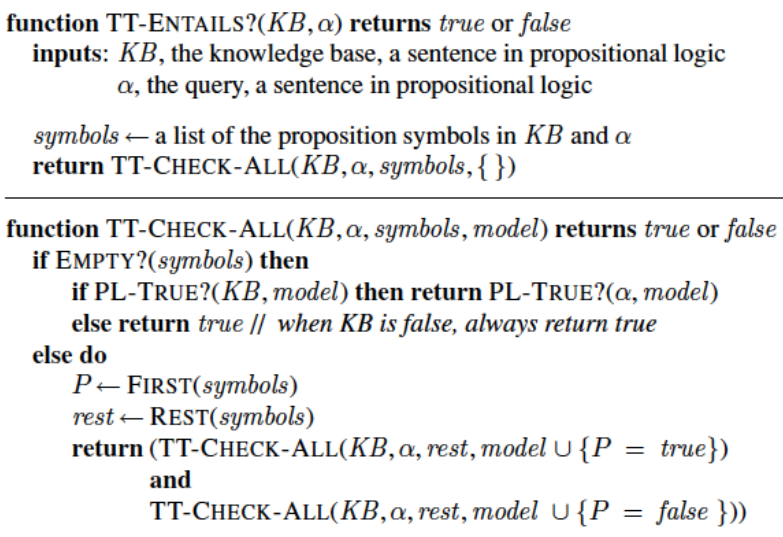
\includegraphics[scale=0.7]{ttentails.png}
\end{center}
\paragraph{Esempio}
\begin{list}{}{($\neg$A $\vee$ B) $\wedge$ (A $\vee$ C) $\vDash$ (B $\vee$ C) ?}
	\item \texttt{TT-CHECK-ALL}( ($\neg$A $\vee$ B) $\wedge$ (A $\vee$ C), (B $\vee$ C), [A, B, C], \{\} )
	\begin{list}{}{}
		\item \texttt{TT-CHECK-ALL}( ($\neg$A $\vee$ B) $\wedge$ (A $\vee$ C), (B $\vee$ C), [B, C], \{A = \textit{true}\} )
		\begin{list}{}{}
			\item \texttt{TT-CHECK-ALL}( ($\neg$A $\vee$ B) $\wedge$ (A $\vee$ C), (B $\vee$ C), [C], \{A = \textit{true}, B = \textit{true}\} )
			\begin{list}{}{}
				\item[OK] \texttt{TT-CHECK-ALL}( ($\neg$A $\vee$ B) $\wedge$ (A $\vee$ C), (B $\vee$ C), [], \{A = \textit{true}, B = \textit{true}, C = \textit{true}\} )
				\item[OK] \texttt{TT-CHECK-ALL}( ($\neg$A $\vee$ B) $\wedge$ (A $\vee$ C), (B $\vee$ C), [], \{A = \textit{true}, B = \textit{true}, C = \textit{false}\} )
			\end{list}
			\item \texttt{TT-CHECK-ALL}( ($\neg$A $\vee$ B) $\wedge$ (A $\vee$ C), (B $\vee$ C), [C], \{A = \textit{true}, B = \textit{false}\} )
			\begin{list}{}{}
				\item[OK] \texttt{TT-CHECK-ALL}( ($\neg$A $\vee$ B) $\wedge$ (A $\vee$ C), (B $\vee$ C), [], \{A = \textit{true}, B = \textit{false}, C = \textit{true}\} )
				\item[OK] \texttt{TT-CHECK-ALL}( ($\neg$A $\vee$ B) $\wedge$ (A $\vee$ C), (B $\vee$ C), [], \{A = \textit{true}, B = \textit{false}, C = \textit{false}\} )
			\end{list}
		\end{list}
		\item \texttt{TT-CHECK-ALL}( ($\neg$A $\vee$ B) $\wedge$ (A $\vee$ C), (B $\vee$ C), [B, C], \{A = \textit{false}\} ) \ldots
	\end{list}
\end{list}
Solo alla fine, \textbf{dopo aver provato tutti i possibili assegnamenti}, possiamo rispondere se (B $\vee$ C) è conseguenza logica.
\section{Algoritmi per la soddisfacibilità (SAT)}
Usano una KB come \textbf{insieme di clausole}, cioè insiemi di letterali:\\\{A, B\} \{$\neg$B, C, D\} \{$\neg$A, F\}\\
La forma a clausole è la \textbf{forma normale congiuntiva} (\textbf{CNF}), cioè una congiunzione di disgiunzioni letterali:\\ 
\{A $\vee$ B\} $\wedge$ \{$\neg$B $\vee$ C $\vee$ D\} $\wedge$ \{$\neg$A $\vee$ F\}\\
\textbf{Non è restrittiva}: è sempre possibile ottenerla con trasformazioni che preservano l'equivalenza logica.
\paragraph{Trasformazione in forma a clausole}
\begin{list}{-}{I passi sono:}
	\item Eliminazione della $\Leftrightarrow$: (A $\Leftrightarrow$ B) $=$ (A $\Rightarrow$ B) $\wedge$ (B $\Rightarrow$ A)
	\item Eliminazione dell'$\Rightarrow$: (A $\Rightarrow$ B) $=$ ($\neg$A $\vee$ B)
	\item Negazioni all'interno (de Morgan):\\
	$\neg$(A $\vee$ B) $=$ ($\neg$A $\wedge$ $\neg$B)\\
	$\neg$(A $\wedge$ B) $=$ ($\neg$A $\vee$ $\neg$B)
	\item Distribuzione di $\vee$ su $\wedge$: (A $\vee$ (B $\wedge$ C)) $=$ (A $\vee$ B) $\wedge$ (A $\vee$ C)
\end{list}
\subsection{Algoritmo DPLL}
\paragraph{DPLL} Davis, Putman, Lovemann, Loveland. Parte da una KB in forma a clausole. Enumerazione in profondità di tutte le possibili interpretazioni alla ricerca di un modello. Tre miglioramenti rispetto TTEntails:
\begin{list}{}{}
	\item \textbf{Terminazione anticipata}: si può decidere sulla verità di una clausola anche con interpretazioni parziali, basta che un letterale sia vero.\\
	Se A è \textit{true}, lo sono anche \{A, B\} e \{A, C\} indipendentemente dai valori di B e di C.\\
	Se anche una sola clausola è falsa, l'interpretazione non può essere un modello dell'insieme delle clausole.
	\item Euristica dei \textbf{simboli} (o letterali) \textbf{puri}: un \textbf{simbolo puro} è un simbolo che \textbf{appare con lo stesso segno in tutte le clausole}. Ad esempio, nella KB \{A, $\neg$B\}, \{$\neg$B, $\neg$C\}, \{C, A\} i simboli A e B sono puri.\\
Nel determinare un simbolo se è puro possiamo trascurare occorrenze simbolo in clausole già rese vere.\\
	Se simbolo è puro può essere assegnato a \textit{true} se positivo e \textit{false} se negativo senza escludere modelli utili: se le clausole hanno un modello continueranno ad averlo anche dopo questo assegnamento. L'assegnamento è obbligato.
	\item Euristica delle \textbf{clausole unitarie}: una \textbf{clausola unitaria} è una \textbf{clausola con un solo letterale non assegnato}. Ad esempio, \{B\} è unitaria, ma anche \{B, $\neg$C\} quando C = \textit{true}.\\
	Conviene assegnare prima valori al letterale in clausole unitarie. L'assegnamento è univoco (\textit{true} se positivo, \textit{false} se negativo)
\end{list}
\begin{center}
	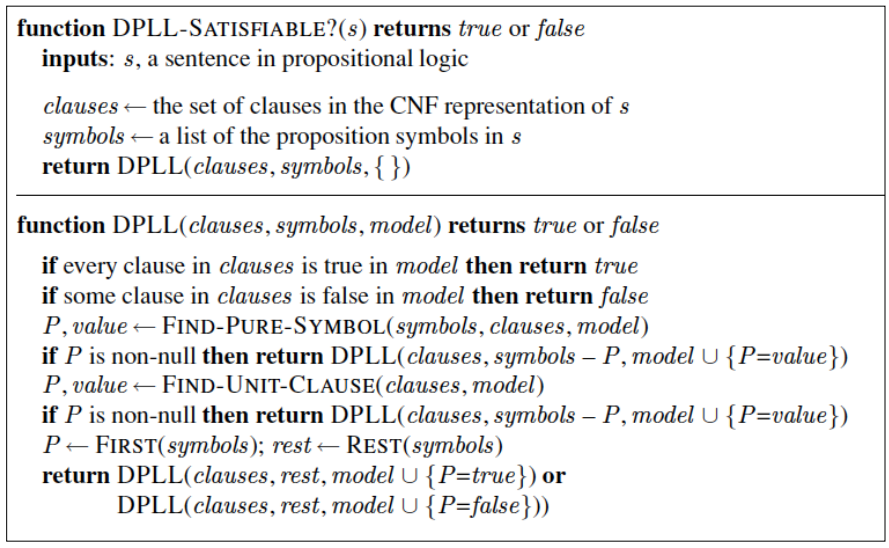
\includegraphics[scale=0.7]{dpllalgoritmo.png}
\end{center}
\paragraph{Miglioramenti di DPLL} DPLL è completo e termina sempre. Alcuni miglioramenti:
\begin{list}{}{}
	\item Analisi di componenti (sottoproblemi indipendenti): se le variabili possono essere suddivise in sottoinsiemi disgiunti
	\item Ordinamento di variabili e valori: scegliere la variabile che compare in più clausole
	\item Backtracking intelligente
	\item Altre ottimizzazioni\ldots
\end{list}
\pagebreak
\subsection{Metodi locali per SAT}
\paragraph{Formulazione}
\begin{list}{}{}
	\item Gli stati sono assegnamenti completi
	\item L'obiettivo è un assegnamento che soddisfa tutte le clausole (un \textbf{modello})
	\item Si parte da un assegnamento casuale
	\item Ad ogni passo \textbf{si cambia il valore di una proposizione} (\textbf{flip})
	\item Gli stati sono valutati contando il numero di clausole non soddisfatte, meno sono meglio è (o soddisfatte)
\end{list}
\paragraph{Algoritmi} Ci sono molti minimi locali, per sfuggire ai quali bisogna introdurre delle perturbazioni casuali. Ad esempio, hill-climbing con riavvio casuale, simulated annealing\ldots\\
C'è stata molta sperimentazione per trovare il miglior compromesso tra il grado di avidità e la casualità.\\
\textbf{WalkSAT} è uno degli algoritmi più semplici ed efficaci.
\subsection{Algoritmo WalkSAT}
Ad ogni passo \textbf{sceglie a caso una clausola non ancora soddisfatta}. Poi \textbf{sceglie un simbolo da modificare} (flip), scegliendo con probabilità $p$ (di solito 0.5) tra una delle due seguenti possibilità:
\begin{list}{}{}
	\item \textbf{Passo casuale}: sceglie un simbolo a caso da flippare
	\item \textbf{Passo di ottimizzazione}: sceglie quello che rende più clausole soddisfatte
\end{list}
Si arrende dopo un numero predefinito di flip.
\begin{center}
	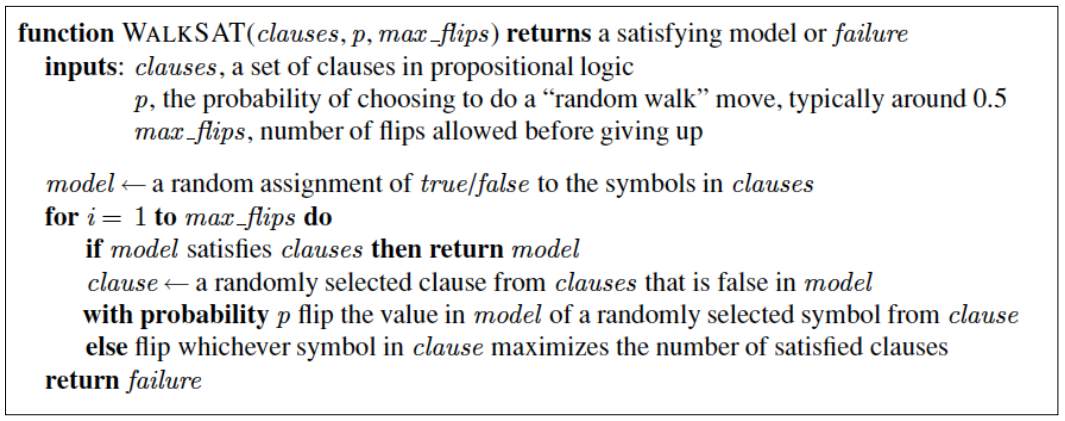
\includegraphics[scale=0.6]{walksatalgoritmo.png}
\end{center}
\paragraph{Analisi} Se \texttt{maxflips} è $\infty$ e l'insieme clausole è soddisfacibile, prima o poi termina. Ma \textbf{non può essere usato per verificare l'insoddisfacibilità} (è \textbf{incompleto}). Il problema è decidibile ma l'algoritmo è incompleto.\\
Va bene per cercare un modello, sapendo che c'è. Ma se è insoddisfacibile, non termina.\\
Lo si usa perché è efficiente in tempo e spazio.
\paragraph{Problemi SAT difficili} Se un problema ha molte soluzioni (sotto-vincolato) è più probabile che WalkSAT ne trovi una in tempi brevi. Per esempio, se ha 16 soluzioni su 32, un assegnamento ha il 50\% di probabilità di essere giusto, quindi \textbf{2 passi in media}.\\
\textbf{Più grande è il rapporto più vincolato è il problema}.
\paragraph{Probabilità di soddisfacibilità in funzione di $\frac{m}{n}$}
\begin{center}
	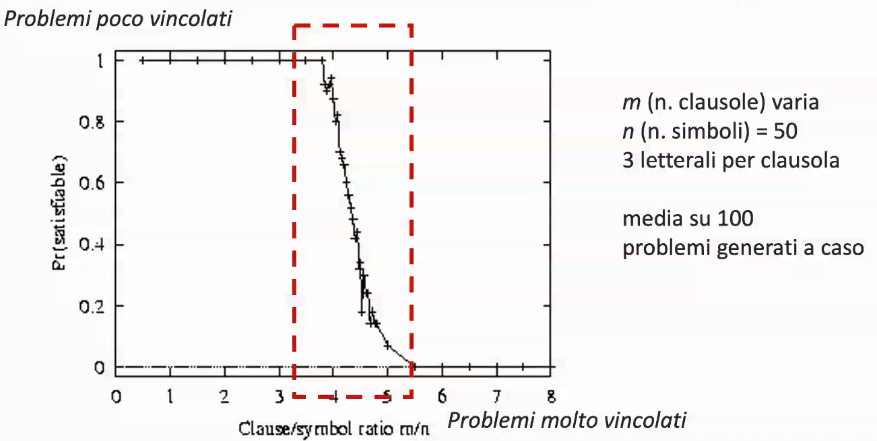
\includegraphics[scale=0.7]{sat_grafico.png}
\end{center}
\paragraph{Confronto tra DPLL e WalkSAT}
\begin{center}
	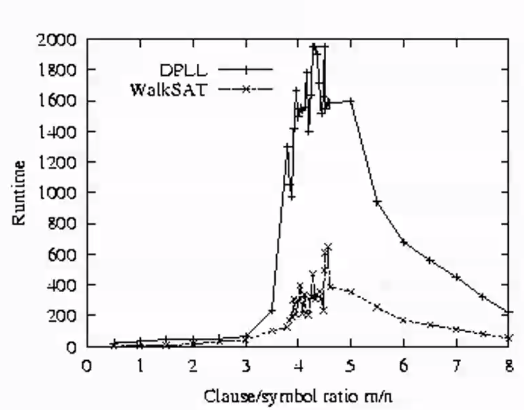
\includegraphics[scale=0.7]{dpllwalksat_confronto.png}
\end{center}
\section{Inferenza come Deduzione}
Un altro modo per decidere se KB $\vDash$ A è usare un meccanismo di \textbf{dimostrazione} (\textbf{deduzione}).\\
Si scrive KB $\vdash$ A (\textbf{A è deducibile da KB}) e la deduzione avviene specificando delle regole di inferenza: dovrebbero derivare solo le formule che sono conseguenza logica e \textbf{tutte} le formule che sono conseguenza logica.\\
Sono le proprietà della \textbf{correttezza} e \textbf{completezza}.
\paragraph{Correttezza} Se KB $\vdash$ A, allora KB $\vDash$ A\\
Tutto ciò che è derivabile è conseguenza logica. Le regole preservano la verità
\paragraph{Completezza} Se KB $\vDash$ A, allora KB $\vdash$ A\\
Tutto ciò che è conseguenza logica è ottenibile tramite il meccanismo di inferenza.\\
\paragraph{Dimostrazione come ricerca}
Come decidere ad ogni passo quale regola di inferenza applicare? A quali premesse? Come evitare esplosione combinatoria? Problema esplorazione spazio di stati. Ci riguarda perché vogliamo progettare algoritmi di inferenza. Una \textbf{procedura di dimostrazione} definisce direzione e strategia di ricerca.
\subparagraph{Direzione} Nella dimostrazione di teoremi \textbf{conviene procedere all'indietro}. Con un applicazione in avanti delle regole di inferenza non controllata posso ottenere, ad esempio da A, B: A $\wedge$ B, A $\wedge$ (A $\wedge$ B)\ldots\\
All'indietro invece, se voglio dimostrare A $\wedge$ B, si cerca di dimostrare A e poi B. Se voglio dimostrare A $\Rightarrow$ B, assumo A e cerco di dimostrare B\ldots
\subparagraph{Strategia} Anche assumendo insieme di regole di inferenza completo se l'algoritmo non è completo potrei non trovare soluzione. La complessità è alta: è un problema \textbf{decidibile ma NP-completo}.
\subsection{Regola di risoluzione per PROP} Meno regole uso meglio è, senza rinunciare alla completezza. L'unica regola di inferenza è la regola di risoluzione, che presuppone la forma a clausole
Con due clausole, una P e l'altra che contiene $\neg$P, possiamo considerare l'OR degli altri elementi togliendo P e $\neg$P. Cioè $$\frac{\{P, Q\}\:\:\{\neg P, R\}}{\{Q, R\}}$$ Corretta? Basta pensare ai modelli.
\subparagraph{In generale} Con $l$, $m$ \textbf{letterali}, simboli di proposizione positivi o negativi. $l_i$ e $m_j$ sono \textbf{uguali ma di segno opposto}.
$$\frac{\{l_1, l_2,\ldots, l_i, \ldots, l_k\}\:\:\{m_1, m_2, \ldots, m_j, \ldots, m_n\}}{\{l_1, l_2,\ldots, l_{i-1}, l_{i+1}, \ldots, l_k, m_1, m_2, \ldots, m_{j-1}, m_{j+1}, \ldots, m_n\}}$$
Caso particolare $\frac{\{P\}\:\:\{\neg P\}}{\{\}}$: \textbf{clausola vuota} o \textbf{contraddizione}.
\paragraph{Grafo di risoluzione}
\begin{center}
	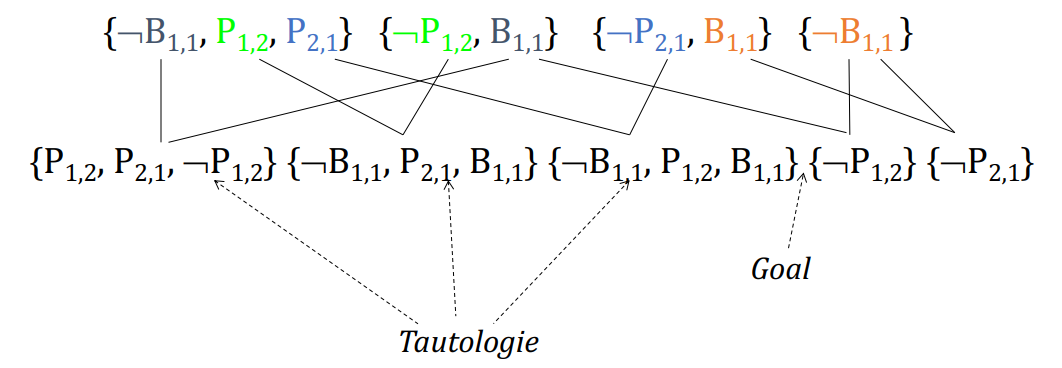
\includegraphics[scale=0.6]{grafosoluz.png}
\end{center}
\paragraph{Attenzione!} \{B, N\} \{$\neg$B, $\neg$N\} $\rightarrow$ \{\} NO!\\
Diventa o \{N,$\neg$N\} \textbf{\textit{oppure}} \{B, $\neg$B\}, \textbf{un passo alla volta}!
\paragraph{Siamo sicuri che basti una regola?} Completezza: KB $\vDash \alpha$ $\Rightarrow$ KB $\vdash_{res} \alpha$? Non sempre. Un controesempio è KB $\vDash$ \{A, $\neg$A\} ma non è vero che KB $\vdash_{res}$ \{A,$\neg$A\}\\
Ma ho due strumenti:
\subparagraph{Teorema di risoluzione} KB insoddisfacibile $\Leftrightarrow$ KB $\vdash_{res}$ \{\} \textbf{completezza}
\subparagraph{Teorema di refutazione} KB $\vDash \alpha \Leftrightarrow$ (KB $\bigcup$ \{$\neg\alpha$\} è insoddisfacibile
\paragraph{Nell'esempio} KB $\bigcup$ FC($\neg$(A or $\neg$A)) è insoddisfacibile? Si, perché
KB $\bigcup$ \{A\} $\bigcup$ \{$\neg$A\} $\vdash_{res}$ \{\} in un passo
\paragraph{Conclusioni}
Abbiamo visto che gli agenti KB che usano il calcolo proposizionale come linguaggio di rappresentazione possono decidere se KB $\vDash \alpha$. Il problema è decidibile ma intrattabile (NP al caso peggiore). Esistono algoritmi efficienti e completi che consentono di affrontare problemi di grosse dimensioni, ed esistono algoritmi locali particolarmente efficienti ma non completi. Oppure per via deduttiva.
\subsection{Logica del Primo Ordine}
%TODO ma è roba saltabile
\subsection{Inferenza nella Logica del Prim'Ordine}
\paragraph{Regole d'inferenza per $\forall$} Istanziazione dell'Universale
$$\frac{\forall\:x\:\:A[x]}{A[g]}$$
Da $\forall\:x\:\:\textsl{King}(x) \wedge \textsl{Greedy}(x) \Rightarrow \textsl{Evil}(x)$ si possono ottenere
\begin{list}{}{}
	\item King(John) $\wedge$ Greedy (John) $\Rightarrow$ Evil(John)
	\item King(Father(John)) $\wedge$ Greedy(Father(John)) $\Rightarrow$ Evil(Father(John))
\end{list}

\paragraph{Regola d'inferenza per $\exists$} Istanziazione dell'Esistenziale
$$\frac{\exists\:x\:\:A[x]}{A[k]}$$
Se $\exists$ non compare nell'ambito di $\forall$, K è una costante nuova (\textbf{costante di Skolem}). Altrimenti va introdotta una funzione (\textbf{di Skolem}) nelle variabili quantificate universalmente
\begin{list}{}{}
	\item $\exists\: x\:\:\textsl{Padre}(x, G)$ diventa $\textsl{Padre(k, G)}$
	\item $\forall\: x\:\:\exists\: y\:\:\textsl{Padre}(x, y)$ diventa $\forall\: x\:\:\textsl{Padre(x, p(x))}$ \textbf{e non} $\forall\: x\:\:\textsl{Padre}(x, k)$ altrimenti tutti avrebbero lo stesso padre
\end{list}
\paragraph{Grounding} Anche detto \textbf{proposizionalizzazione}: creo tante istanze delle formule quantificate universalmente quanti sono gli oggetti menzionati ed elimino i quantificatori esistenziali \textbf{skolemizzando}.\\
La KB diventa proposizionale e possiamo applicare gli algoritmi visti. Sorgono dei problemi: le costanti sono in numero finito, ma \textbf{se ci sono delle funzioni il numero delle istanze da creare diventa infinito} (John, Padre(John), Padre(Padre(John)),\ldots)
\subsection{Teorema di Herbrand}
Se KB $\vDash$ A $\Rightarrow$ \textbf{c'è una dimostrazione che coinvolge solo un sottoinsieme finito della KB proposizionalizzata}.\\
Si può procedere in modo incrementale
\begin{list}{}{}
	\item Creo le istanze con le costanti
	\item Creo quelle con un solo livello di annidamento: Padre(John), Madre(John)
	\item Creo quelle con due livelli di annidamento: Padre(Padre(John)), Padre(Madre(John)), Madre(Padre(John)), Madre(Madre(John))
\end{list}
Se KB $\not\vDash$ A, il processo non termina $\Rightarrow$ \textbf{semidecidibile}.
\subsection{Regola di risoluzione per il FOL}
Abbiamo visto la regola di risoluzione per il PROP, un metodo deduttivo corretto e completo con un'unica regola. Possiamo estenderla al FOL? Si, ma per definirla dobbiamo estendere al FOL la trasformazione in forma a clausole e introdurre il concetto di unificazione.
\pagebreak
\paragraph{Forma a clausole}
Costanti, funzioni e predicati sono come definiti prima, ma \textbf{escludiamo la formule atomiche del tipo ($t_1$ = $t_2$)}.
\paragraph{Clausola} \textbf{Una clausola è insieme di letterali} (formula atomica eventualmente negata) \textbf{che rappresenta la loro disgiunzione}.\\
Una KB è un insieme di clausole.
\begin{list}{}{}
	\item Clausola $\Rightarrow$ \{Letterale, \ldots, Letterale\}
	\item Letterale $\Rightarrow$ FormulaAtomica $|$ $\neg$FormulaAtomica
\end{list}
\subsubsection{Trasformazione in forma a clausole}
\paragraph{Teorema} $\forall$ formula chiusa $\alpha$ del FOL, è possibile trovare in maniera \textbf{effettiva} un insieme di clausole FC($\alpha$) soddisfacibile $\Leftrightarrow \alpha$ era soddisfacibile (viceversa, insoddisfacibile $\Leftrightarrow \alpha$ era insoddisfacibile)
\paragraph{Esempio trasformazione} Vediamo un esempio per la frase "\textit{tutti coloro che amano tutti gli animali sono amati da qualcuno}".
$$\forall\: x (\forall\: y\:\:\textsl{Animale}(y) \Rightarrow Ama(x, y)) \Rightarrow (\exists\: y\:\:Ama(y, x))$$
\begin{enumerate}
	\item \textbf{Eliminazione delle implicazioni} $\Rightarrow$ e $\Leftrightarrow$:\\
	$A \Rightarrow B$ diventa $\neg A \vee B$, 	$A \Leftrightarrow B$ diventa $(\neg A \vee B) \wedge (\neg B \vee A)$.
	\begin{list}{}{}
		\item $\forall\: x (\forall\: y\:\:\textsl{Animale}(y) \Rightarrow Ama(x, y)) \underline{\Rightarrow} (\exists\: y\:\:Ama(y, x))$
		\item $\forall\: x \neg(\forall\: y\:\:\textsl{Animale}(y) \underline{\Rightarrow} Ama(x, y)) \vee (\exists\: y\:\:Ama(y, x))$
		\item $\forall\: x \neg(\forall\: y\:\:\neg\textsl{Animale}(y) \vee Ama(x, y)) \vee (\exists\: y\:\:Ama(y, x))$
	\end{list}
	\item \textbf{Negazioni all'interno}:
	$\neg\neg A$ diventa $A$\\
	$\neg(A \wedge B)$ diventa $\neg A \vee \neg B$ (De Morgan)\\
	$\neg(A \vee B)$ diventa $\neg A \wedge \neg B$ (De Morgan)\\
	$\neg\forall x\:A$ diventa $\exists x\:\neg A$, $\neg\exists x\:A$ diventa $\forall x\:\neg A$
	\begin{list}{}{}
		\item $\forall\: x \underline{\neg}(\forall\: y\:\:\neg\textsl{Animale}(y) \vee Ama(x, y)) \vee (\exists\: y\:\:Ama(y, x))$
		\item $\forall\: x (\exists\: y\:\:\underline{\neg}(\neg\textsl{Animale}(y) \vee Ama(x, y))) \vee (\exists\: y\:\:Ama(y, x))$
		\item $\forall\: x (\exists\: y\:\:(\textsl{Animale}(y) \wedge \neg Ama(x, y))) \vee (\exists\: y\:\:Ama(y, x))$
	\end{list}
	\item \textbf{Standardizzazione delle variabili}: ogni quantificatore una variabile diversa
	\begin{list}{}{}
		\item $\forall\: x (\exists\: y\:\:(\textsl{Animale}(y) \wedge \neg Ama(x, y))) \vee (\exists\: z\:\:Ama(z, x))$
	\end{list}
	\item \textbf{Skolemizzazione}: eliminazione di quantificatori esistenziali.\\
	Ci sono due quantificatori esistenziali nell'ambito di uno universale, dobbiamo introdurre due funzioni di Skolem
	\begin{list}{}{}
		\item $\forall\: x (\textsl{Animale}(F(x)) \wedge \neg Ama(x, F(x))) \vee (Ama(G(x), x))$
	\end{list}
	\item \textbf{Eliminazione di quantificatori universali}\\
	Possiamo portarli tutti davanti (forma premessa) ed eliminarli usando la convenzione che le variabili libere sono quantificate universalmente.\\
	Se B non contiene $x$\\
	$(\forall x\:A) \vee B$ diventa $\forall x\:(A \vee B)$, $(\forall x\:A) \wedge B$ diventa $\forall x\:(A \wedge B)$
	\begin{list}{}{}
		\item $\underline{\forall\: x} (\textsl{Animale}(F(x)) \wedge \neg Ama(x, F(x))) \vee (Ama(G(x), x))$
		\item $(\textsl{Animale}(F(x)) \wedge \neg Ama(x, F(x))) \vee (Ama(G(x), x))$
	\end{list}
	\item \textbf{Forma normale congiuntiva}: congiunzioni di disgiunzioni letterali\\
	$A \vee (B \wedge C)$ diventa $(A \vee B) \wedge (A \vee C)$
	Quindi
	\begin{list}{}{}
		\item $(\textsl{Animale}(F(x)) \underline{\wedge} \neg Ama(x, F(x))) \underline{\vee} (Ama(G(x), x))$
		\item $(\textsl{Animale}(F(x)) \vee \neg Ama(G(x), x)) \wedge ((\neg Ama(x, F(x)) \vee Ama(G(x), x)))$
	\end{list}
	\pagebreak
	\item \textbf{Notazione a clausole}
	\begin{list}{}{}
		\item \{Animale$(F(x))$, Ama$(G(x), x)$\}
		\item \{$\neg$Ama$(x, F(x))$, Ama$(G(x), x)$\}
	\end{list}
	\item \textbf{Separazione delle variabili}: clausole diverse, variabili diverse\\
	$\forall x\: (P(x) \wedge Q(x)) \Leftrightarrow \forall x_1\: P(x_1) \wedge \forall x_2\:Q(x_2)$
	\begin{list}{}{}
		\item \{Animale$(F(x))$, Ama$(G(x), x)$\} $\longrightarrow$ \{Animale$(F(x_1))$, Ama$(G(x_1), x_1)$\}
		\item \{$\neg$Ama$(x, F(x))$, Ama$(G(x), x)$\} $\longrightarrow$ \{$\neg$Ama$(x_2, F(x_2))$, Ama$(G(x_2), x_2)$\}
	\end{list}
\end{enumerate}
\textbf{La Skolemizzazione non preserva l'equivalenza}: $P(a) \vDash \exists x\:P(x)$ ma $\exists x\:P(x) \not\vDash P(x)$
\paragraph{Unificazione} Operazione con la quale si determina se due espressioni possono essere rese identiche mediante una sostituzione di termini a variabili.\\
Il risultato è la sostituzione che rende le due espressioni identiche, detta \textbf{unificatore}, o \textbf{FAIL} se le espressioni non sono unificabili.
\paragraph{Sostituzione} Insieme finito di associazioni tra variabili e termini in cui ogni variabile compare una sola volta sulla sinistra. Es \{x$_1$/A, x$_2$/f(x$_3$), x$_3$/B\} significa che A va sostituita a x$_1$, f(x$_3$) sostituita a x$_2$\ldots\\
A sinistra vanno le variabili e a destra costanti e variabili, con la restrizione che la variabile sulla sinistra non può comparire anche sulla destra della stessa "coppia".
\paragraph{Applicazione} Sia $\sigma$ una sostituzione e A espressione, A$\sigma$ è l'istanza generala dalla sostituzione (delle variabili con l'espressione corrispondente)\\
In AIMA \texttt{SUBST($\sigma$, A)}. Le variabili sono \textbf{sostituite simultaneamente} e si esegue un solo passo di sostituzione
\paragraph{Espressioni unificabili} Se esiste una sostituzione che le rende identiche, cioè se esiste un unificatore.\\
In genere l'unificatore $\tau$ non è unico, quindi vorremmo l'unificatore più generale di tutti (MGU). \textbf{Teorema}: l'\textbf{unificatore più generale è unico} a meno dei nomi delle variabili (l'ordine non conta).
\paragraph{Algoritmo di unificazione} Input: p, q espressioni.\\
Output: MGU $\theta$ se esiste (\texttt{unify(p,q) = $\theta$} tale che \texttt{subst($\theta$, p) = subst($\theta$, q)}) altrimenti \textbf{FAIL}.\\
Esplora in parallelo le due espressioni e costruisce l'unificatore strada facendo. Fallisce non appena trova due espressioni non unificabili. Una causa del fallimento sono le sostituzioni del tipo $x = f(x)$: questo controllo si chiama \textbf{occurr-check}.
\begin{center}
	\begin{lstlisting}
function UNIFY(x, y, theta) returns una sostituzione
	# theta, la sostituzione costruita fin'ora (opzionale, vuota di default)
	if theta = FAIL then return FAIL
	else if x = y: return theta
	else if VARIABLE?(x): return UNIFY-VAR(x, y, theta)
	else if VARIABLE?(y): return UNIFY-VAR(y, x, theta)
	else if COMPOUND?(x) and COMPOUND?(y):
		return UNIFY(x.ARGS, y.ARGS, UNIFY(x.OP, y.OP, theta))
	else if LIST?(x) and LIST?(y):
		return UNIFY(x.REST, y.REST, UNIFY(x.FIRST, y.FIRST, theta))
	else return FAIL

function UNIFY-VAR(var, x, theta) returns una sostituzione
	if {var/val} in theta: return UNIFY(val, x, theta) # var ha gia un valore
	else if {x/val} in theta: return UNIFY(var, val , theta) # x ha gia un valore
	else if OCCUR-CHECK?(var, x): return FAIL # controllo di occorrenza
	else return EXTEND({var/x} , theta)
	\end{lstlisting}
\end{center}
\texttt{OCCURR-CHECK} controlla se \texttt{var} occorre all'interno dell'espressione $x$. In tal caso, fallisce. Controllo di complessità quadratica.\\
\textbf{Attenzione}: \texttt{EXTEND} non aggiunge semplicemente ma applica la sostituzione in $\theta$.
%TODO esempi
\section{Definizione e Confronto di Euristiche Ammissibili}
\paragraph{Mondo dei blocchi} Problema classico, parte dei micromondi usati soprattutto per la pianificazione. Serie di blocchi su un tavolo impilati e vogliamo raggiungere certa config. final. Mosse sono spostare blocco su tavolo o su altro blocco, a condizione che blocco sia libero senza blocchi sopra e blocco destinazione anche.
\subparagraph{Euristica H1} Numero di blocchi appoggiati su blocco sbagliato (incluso tavolo)
\subparagraph{Euristica H2} Numero blocchi con supporto (torre sotto) sbagliato
\subparagraph{Sono ammissibili?} Sono ammissibili se servono almeno Hi mosse per giungere in stato goal. H2 è più accurata perché domina H1, valore più alto per ogni stato possibile. Questo perché H2 $\Rightarrow$ H1, i blocchi contati in H1 vengono contati anche in H2, ma H2 ha casi non contati da H1.\\
Per trovare euristica bisogna contare quanto dista soluzione e usare questa come euristica.\\
Euristica = n ammissibile se servono almeno n mosse per arrivare in stato finale, $\geq$ 0 ovunque ma $=$ 0 solo in stati goal.

\chapter{Strategie di risoluzione}
\paragraph{Fin'ora} Abbiamo visto metodi di risoluzione per le KB in forma a clausole: l'unificazione e la regola di risoluzione per FOL (estensione rispetto alla regola PROP).\\
\textbf{Come rendere più efficiente il meccanismo di risoluzione}? Bisogna adottare strategie di risoluzione: tecniche per esplorare in maniera efficiente il grafo di risoluzione, possibilmente senza perdere la completezza.\\
Un percorso che ci porterà a giustificare i sistemi a regole e le restrizioni del FOL associate.
\section{Strategia di risoluzione}
Distinzione tra 
	\begin{list}{}{}
		\item \textbf{Strategie di cancellazione}: \textit{ci sono clausole che possiamo eliminare}?
		\item \textbf{Strategie di restrizione}: \textit{posso usare ad ogni passo solo alcune clausole}?
		\item \textbf{Strategie di ordinamento}: \textit{posso "risolvere" i letterali in un ordine specifico}?
	\end{list}
Tutto possibilmente \textbf{senza perdere completezza}
\subsection{Strategie di Cancellazione}
Consiste nel \textbf{rimuovere} dalla KB, ai fini della dimostrazione, \textbf{le clausole che non saranno mai utili nel processo di risoluzione}.
\begin{list}{}{}
	\item \textbf{Clausole con Letterali Puri}\\
	Letterali che non hanno il loro negato nella KB\\
	$\{\neg P, \neg Q, R\}\:\{\neg P, \underline{S}\}\:\{\neg Q, \underline{S}\}\:\{P\}\:\{Q\}\:\{\neg R\}$\\
	Non potranno mai essere risolte con altre clausole per ottenere \{\}, tanto vale eliminarle. Non si perdono soluzioni
	\item \textbf{Tautologie}\\
	Clausole con due letterali identici e complementari\\
	$\{\underline{P(A)}, \underline{\neg P(A)}, \ldots\}\:\{P(x), \underline{Q(y)}, \underline{\neg Q(y)}\}$\\
	\textbf{Nota}: non basta che siano unificabili e di segno opposto\\
	$\{\underline{\neg P(A)}, \underline{P(x)}\}\:\{P(A)\}\:\{\neg P(B)\}$ è insoddisfacibile\\
	$\{P(A)\}\:\{\neg P(B)\}$ è soddisfacibile\\	
	Le tautologie \textbf{possono essere generate}, quindi questo controllo deve essere eseguito ad ogni passo
	\item \textbf{Clausole Sussunte} (implicate)\\
	$P(x)$ \textit{sussume} $P(A)$, $P(A)$ \textit{sussume} $\{P(A), P(B)\}$\\
	In generale $\alpha$ \textbf{sussume} $\beta \Leftrightarrow \exists\:\sigma$ con $\alpha\sigma \subset \beta$, cioè se un'istanza di $\alpha$ con la sostituzione $\sigma$ è un sottoinsieme di $\beta$. Ad esempio\\
	$\{P(x), Q(y)\}$ sussume $\{P(A), Q(v), R(w)\}$ infatti $\{P(x), Q(y)\}\{x/A, y/v\}=\{P(A), Q(v)\}\:\subset\:\{P(A), Q(v), R(w)\}$\\
	$\beta$ può essere ricavata da $\alpha$, quindi $\beta$ può essere eliminata senza perdere soluzioni. Anche le clausole sussunte possono essere generate.
\end{list}
\pagebreak
\subsection{Strategie di Restrizione}
Ad ogni passo si sceglie tra un sottoinsieme di possibili clausole
\begin{list}{}{}
	\item \textbf{Risoluzione unitaria}\\
	\textbf{Almeno una delle due clausole} utilizzate nel passaggio \textbf{è unitaria} (un solo letterale)
	\begin{center}
		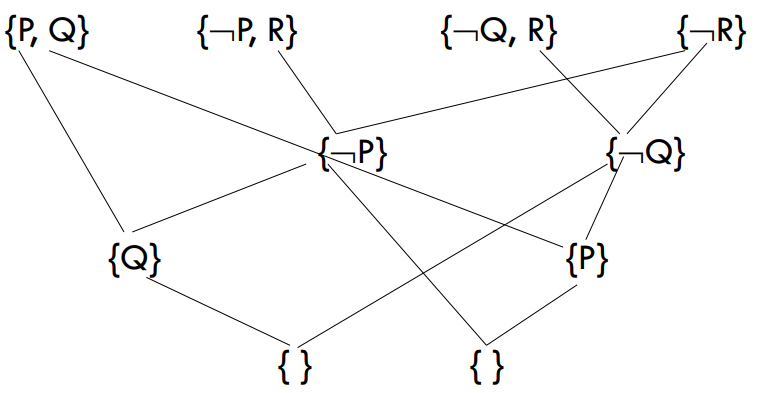
\includegraphics[scale=0.5]{risunit.png}
	\end{center}
	\textbf{Converge molto rapidamente}, perché ad ogni passo si elimina una clausola, ed è facile da implementare. Ma non è completa, esempio: $\{P, Q\}\:\{\neg P, Q\}\:\{P, \neg Q\}\:\{\neg P, \neg Q\} \vdash_{RES} \{\}$ non con risoluzione unitaria.\\
	Completa per \textbf{Clausole di Horn}: clausole con \textbf{al più} un letterale positivo
	\item \textbf{Risoluzione lineare}\\
	Prendo l'ultima clausola generata con una clausola da input (della KB iniziale), oppure una clausola antenata nella sequenza. Completa per la risoluzione per refutazione.
	\begin{center}
		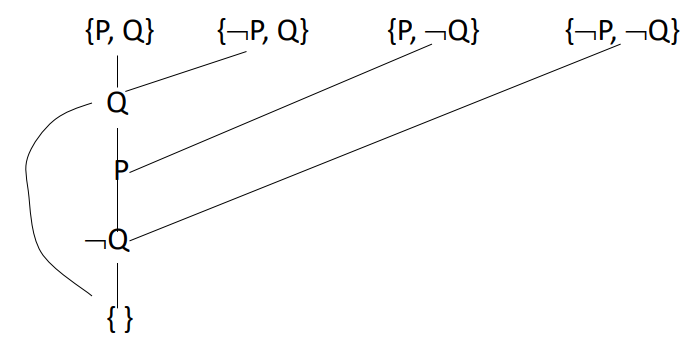
\includegraphics[scale=0.5]{rislin.png}
	\end{center}
	\item \textbf{Risoluzione guidata dal goal}/da insieme di supporto (sottoinsieme della KB responsabile dell'insoddisfacibilità)\\
	Almeno una delle due clausole appartiene a questo insieme o a suoi discendenti\\
	Tipicamente, assumendo la KB iniziale consistente, \textbf{si sceglie come insieme di supporto iniziale il negato della clausola goal}. Il risultato è che è come procedere all'indietro dal goal. Strategia completa, per la refutazione.\\
	\begin{center}
		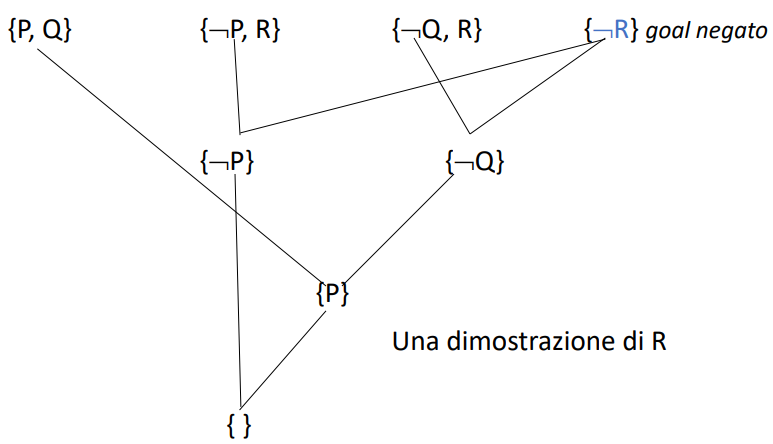
\includegraphics[scale=0.5]{risgoal.png}
	\end{center}
\end{list}
\pagebreak
\subsection{Strategie di Ordinamento}
\begin{list}{}{}
	\item \textbf{Risoluzione ordinata}\\
	Ogni clausola è un \textbf{insieme ordinato} di letterali e \textbf{si possono unificare solo i primi letterali} delle clausole. L'ordinamento deve essere rispettato nel risolvente.
	\begin{multicols}{2}
	\begin{center}
		\includegraphics[scale=0.5]{risord.png}
	\end{center}
	\begin{center}
		\includegraphics[scale=0.4]{risordes.png}
	\end{center}
	\end{multicols}
	La risoluzione ordinata è completa per le clausole Horn
\end{list}
\subsection{Sottoinsieme a regole del FOL}
\paragraph{Clausole di Horn \textit{definite}} Clausole con \textbf{esattamente} un letterale positivo.\\
Possno essere riscritte come fatti e regole:
\begin{list}{}{}
	\item $\neg P_1 \vee \ldots \vee \neg P_k \vee Q$
	\item $\neg (P_1 \wedge \ldots \wedge P_k) \vee Q$
\end{list}
Una \textbf{KB a regole}
\begin{list}{}{}
	\item \textbf{Regola}: $P_1 \wedge \ldots \wedge P_k \Rightarrow Q$
	\item \textbf{Fatto}: $Q$
\end{list}
\subsection{Sistemi a regole logici}
Se la KB contiene solo clausole Horn definite, i meccanismi inferenziali sono molto più semplici ed il processo è molto più guidato, senza rinunciare alla completezza: risolutori in tempo lineare per il caso proposizionale. \textbf{Nota}: è restrittivo e non coincide né con il PROP né con il FOL.
\paragraph{Uso delle regole in avanti e indietro}
\begin{list}{}{}
	\item \textbf{Backward Chaining}: un'istanza di ragionamento \textbf{guidato dall'obiettivo}.\\
	Le regole sono applicate alla rovescia: \textbf{programmazione logica} (PROLOG ha le KB a regole e procede applicando le regole in avanti o all'indietro)
	\item \textbf{Forward Chaining}: un'istanza di ragionamento o ricerca \textbf{guidato dai dati}\\
	Le regole sono applicate nel senso "antecedente-conseguente". Basi di dati deduttive e sistemi di produzione.
\end{list}
\subsection{Programmazione Logica}
I \textbf{programmi logici} sono KB costituite di clausole Horn definite, espressi come fatti e regole con sintassi alternativa:\\
$A :- B_1, B_2, \ldots, B_n$ ($A$ \textbf{testa}, $B_1, \ldots, B_n$ \textbf{corpo})\\
$A$ \textbf{vero} se sono veri $B_1, \ldots, B_n$, in accordo al significato logico di implicazione. Questa è la \textbf{interpretazione dichiarativa}.\\
\textbf{Interpretazione procedurale}: la testa può essere vista come una \textbf{chiamata di procedura} e il corpo come una serie di procedure da eseguire in sequenza.\\
Altre convenzioni: in PL le variabili sono indicate con le lettere maiuscole e le costanti con le lettere minuscole
\subsection{Risoluzione SLD}
\paragraph{Selection Linear Definit-Clauses} Strategia \textbf{lineare} nell'input e  \textbf{ordinata}, \textbf{basata su un insieme di supporto} (la clausola goal).\\SLD è \textbf{completa per clausole Horn}.
\paragraph{Alberi di Risoluzione SLD} Dato un programma logico P, l'\textbf{albero SLD per un goal G} è definito come segue:
\begin{list}{}{}
	\item Ogni nodo dell'albero corrisponde ad un goal (\textbf{congiuntivo})
	\item La radice è \texttt{:- G$_1$, G$_2$, \ldots, G$_k$}, il nostro goal
	\item Sia \texttt{:- G$_1$, G$_2$, \ldots, G$_k$} un nodo dell'albero: il \textbf{nodo ha tanti discendenti quanti sono i fatti e le regole in P la cui testa è unificabile con \texttt{G$_1$}}\\
	Se \texttt{A :- B$_1$, \ldots, B$_k$} $\wedge$ \texttt{A} unificabile con \texttt{G$_1$} $\wedge \gamma =$ MGU(\texttt{A, G$_1$}) $\Rightarrow$ un discendente\\
	è il goal \texttt{:- (B$_1$, \ldots, B$_k$, G$_2$, \ldots, G$_k$)$\gamma$}
	\item I nodi che sono \textbf{clausole vuote} sono \textbf{successi}
	\item I \textbf{nodi che non hanno successori} sono \textbf{fallimenti}
\end{list}
\subparagraph{Esempio}
\begin{enumerate}
	\item Genitore(X, Y) :- Padre(X, Y)
	\item Genitore(X, Y) :- Madre(X, Y)
	\item Antenato(X, Y) :- Genitore(X, Y)
	\item Antenato(X, Y) :- Genitore(X, Z), Antenato(Z, Y)
	\item Padre(Gio, Mark)
	\item Padre(Gio, Luc)
	\item Madre(Lia, Gio)\\
	\item :- Antenato(Lia, Mark) \textit{goal negato}
\end{enumerate}
\begin{center}
\includegraphics[scale=0.7]{sldesempio.png}
\end{center}
\pagebreak
\paragraph{Risoluzione SLD} Strategia completa per clausole Horn definite.\\
Se $P \cup \{\neg G\}$ è insoddisfacibile, allora una delle foglie deve essere la clausola vuota (successo).\\
\textbf{Non è restrittivo andare in ordine} nel risolvere i sottogoal in $\wedge$. La sostituzione corrispondente è la \textbf{risposta calcolata}.
\paragraph{Strategia di visita dell'albero SLD e PROLOG} A seconda di come viene visitato l'albero, la clausola vuota potrebbe non essere trovata: la strategia di ricerca può essere la responsabile dell'incompletezza.\\
In Prolog la visita dell'albero di risoluzione avviene con una ricerca in profondità e backtracking su fallimento, quindi non è una strategia completa. Il programmatore ha la possibilità di controllare l'ordine di generazione perché le regole sono applicate nell'ordine in cui sono scritte nel file.
\section{Sistemi a Regole in Avanti}
\paragraph{Modus Ponens Generalizzato}
$$\frac{p_1'\: p_2'\: \ldots\: p_n'\:\:(p_1\wedge p_2\wedge\ldots\wedge p_n\Rightarrow q)}{(q)\:\Theta} $$
Dove $\Theta$ = MGU($p_i', p_i$) $\forall\: i$\\
\begin{list}{}{Regola \textbf{corretta}:}
	\item Si istanziano gli universali
	\item Si istanziano le regole
	\item Si applica il Modus Ponens classico
\end{list}
Più in generale di MP, ma anche più limitata nella forma del conseguente
\paragraph{Esempio} Supponiamo di avere nella KB:
\begin{list}{}{}
	\item King(John)
	\item Greedy(y)
	\item King(x) $\wedge$ Greedy(x) $\Rightarrow$ Evil(x)
\end{list}
Con $\Theta$ = \{x/John, y/John\} si ottiene
\begin{list}{}{}
	\item King(John), Greedy(John), King(John) $\wedge$ Greedy(John) $\Rightarrow$ Evil(John)
\end{list}
Quindi la conclusione della regola è 
\begin{list}{}{}
	\item Evil(John)
\end{list}
\paragraph{Concatenazione in avanti} Un semplice processo inferenziale (FOL FC Ask) \textbf{applicaripetutamente il Modus Ponens generalizzato} per ottenere nuovi fatti, fino a che:
\begin{list}{}{}
	\item Si dimostra quello che si desidera
	\item Nessun fatto nuovo può essere raggiunto
\end{list}
Strategia di \textbf{ricerca sistematica in ampiezza}
\subparagraph{Esempio}
"\textit{È un crimine per un Americano vendere armi a una nazione ostile. Il
paese Nono, un nemico dell’America, ha dei missili, e tutti i missili gli
sono stati venduti dal colonnello West, un Americano.}"\\
\textbf{Dimostrare} che \textit{West è un criminale}. \textbf{Formalizzazione}:
\begin{enumerate}
	\item Americano(x) $\wedge$ Arma(y) $\wedge$ Vende(x, y, z) $\wedge$ Ostile(z) $\Rightarrow$ Criminale(x)
	\item $\exists$x Possiede(Nono,x) $\wedge$ Missile(x)\\
	Possiede(Nono, M$_1$) $\wedge$ Missile(M$_1$)
	\item Missile(x)$\wedge$Possiede(Nono,x) $\Rightarrow$ Vende(West, x, Nono)
	\item Missile(x) $\Rightarrow$ Arma(x)
	\item Nemico(x, America) $\Rightarrow$ Ostile(x)
	\item Americano(West)
	\item Nemico(Nono, America)
\end{enumerate}
In questo caso non ci sono funzioni ed il processo converge: siamo nelle condizioni di un database Datalog (database deduttivi). \textbf{Prima iterazione}
\begin{enumerate}
	\item Possiede(Nono, M$_1$) $\wedge$ Missile(M$_1$)
	\item Missile(x)$\wedge$Possiede(Nono,x) $\Rightarrow$ Vende(West,x,Nono)\\
	La regola 3 è soddisfatta con \{x/M$_1$\} e viene aggiunto Vende(West, M$_1$, Nono)
	\item Missile(x) $\Rightarrow$ Arma(x)\\
	La regola 4 è soddisfatta con \{x/M$_1$\} e viene aggiunto Arma(M$_1$)
	\item Nemico(x, America) $\Rightarrow$ Ostile(x)
	\item Nemico(Nono, America)\\
	La regola 5 è soddisfatta con \{x/Nono\} e viene aggiunto Ostile(Nono)
\end{enumerate}
\textbf{Seconda iterazione}
\begin{enumerate}
	\item Americano(x) $\wedge$ Arma(y) $\wedge$ Vende(x, y, z) $\wedge$ Ostile(z) $\Rightarrow$ Criminale(x)\\
	La regola 1 è soddisfatta con \{x/West, y/M$_1$, z/Nono)\} e Criminale(West) viene aggiunto
\end{enumerate}
\begin{center}
	\includegraphics[scale=0.7]{westdiminavanti.png}\\
	\textit{Si parte dal basso}
\end{center}
\subsection{Analisi di FOL-FC-Ask}
\textbf{Corretta} perché il Modus Ponens Generalizzato è corretto.\\
\textbf{Completa} per KB di clausole Horn definite:
\begin{list}{}{}
	\item Completa e convergente per calcolo proposizionale e per KB di tipo Datalog (senza funzioni) perché la chiusura deduttiva è un insieme finito
	\item Completa anche con funzioni ma il processo potrebbe non terminare (semidecidibile)
\end{list}
Il metodo descritto è \textbf{sistematico ma non troppo efficiente}.
\subsection{FC Efficiente}
\paragraph{Ordinamento dei congiunti} Conviene \textbf{soddisfare prima i congiunti con meno istanze nella KB} e che compaiono in più regole: Missile(x) $\wedge$ Possiede(Nono,x) $\Rightarrow$ Vende(West,x,Nono) (Tipi di missile $<<$ cose possedute)\\
Altre ottimizzazioni sono mutuate dai CSP.
\pagebreak
\paragraph{Rete di discriminazione} Assunzione: regole diverse possono condividere molte delle precondizioni. Ad esempio:
\begin{list}{}{}
	\item[R1] (Mammifero x) (Felino x) (Carnivoro x)\\
	(A-Macchie x) $\Rightarrow$ (assert (Leopardo x))
	\item[R2] (Mammifero x) (Felino x) (Carnivoro x)\\
	(A-Strisce x) $\Rightarrow$ (assert (Tigre x))
\end{list}
\textbf{Idea}: codificare gli antecedenti delle regole sotto forma di rete di discriminazione.
\begin{center}
	\includegraphics[scale=0.7]{fcdiscriminazione.png}
\end{center}
\paragraph{Incrementale} Ogni nuovo fatto inferito al tempo $t$ deve essere dedotto usando almeno un fatto dedotto al tempo $t-1$\\
Si possono guardare solo le regole che hanno premesse unificabili con fatti aggiunti nell'ultima iterazione.\\
Indicizzare le regole sui fatti, evitare di ricalcolare le unificazioni\ldots\\
Altre ottimizzazioni presenti nell'algoritmo \texttt{RETE}\ldots
\paragraph{Ridurre deduzioni irrilevanti} Un modo per evitare di ricavare fatti irrilevanti: \textbf{lavorando all'indietro dal goal}, non c'è questo problema. Si fa una specie di \textbf{pre-processing per individuare le regole che servono}, procedendo all'indietro dal goal e \textbf{marcando le regole utili}. Poi si procede in avanti \textbf{utilizzando solo le regole marcate}.
\paragraph{\textit{Magic Set}} Dato il goal: Criminal(West), creo una KB $\leftarrow$ KB $\cup$ \{Magic(West)\}. \textbf{Riscrittura delle regole}:
\begin{list}{}{}
	\item Magic(x) $\wedge$ Americano(x) $\wedge$ Arma(y) $\wedge$ Vende(x, y, z) $\wedge$ Ostile(z) $\Rightarrow$ Criminale(x)
\end{list}
Procedendo poi in avanti saranno utilizzate solo le "\textit{regole magiche}" in modo mirato.\\
Combina BC con FC.
\chapter{Machine Learning}
\section{Introduzione al Machine Learning}
\paragraph{Apprendimento} Principio universale che riguarda gli esseri viventi, al cuore del problema dell'intelligenza sia biologica che artificiale.\\
L'apprendimento è una sfida strategica per fornire \textbf{intelligenza} ai sistemi.\\
Si tratta di un problema complesso, campo che cresce continuamente e riguarda aspetti teorici e applicativi: apprendimento automatico / \textbf{machine learning}.\\
Nasce con lo scopo di combinare le ambizioni di creare macchine che possono apprendere con sistemi statistici potenti \textbf{utilizzabili in vari ambiti} con approfondimento rigoroso nella scienza computazionale.
\paragraph{Macchine che imparano da sé} Perché? Lusso o necessità?
\begin{list}{-}{}
	\item Crescente disponibilità e bisogno di analisi di dati empirici
	\item Ruolo centrale e metodologico per il \textbf{cambio di paradigma della scienza}: \textbf{data-driven}
	\item Difficile fornire intelligenza attraverso la programmazione (vedi Turing).\\
	Ha molto più senso lasciare che le macchine apprendano da sole, \textit{non si può insegnare loro tutto}
	\item L'apprendimento è l'unica via\ldots
\end{list}
Dati + HPC + ML moderno $\rightarrow$ strada verso la nuova era delle IA
\begin{list}{}{\textbf{Obiettivi}}
	\item Costruire sistemi intelligenti adattivi
	\item Data Analysis per costruire sistemi predittivi potenti, strumenti per i data scientist
	\item Modelli come strumenti per risolvere problemi complessi ed interdisciplinari
\end{list}
Apprendimento automatico di un sistema dell'esperienza (serie di esempi) per affrontare un task computazionale. \textbf{Partire da esempi}
\paragraph{Esempio} \textbf{Classificare lo spam}: collezionare 100 mail di spam, 100 non di spam e le uso come esempi che fornisco al sistema: esso apprende dagli esempi per poter essere capace di classificare in futuro spam e non.
\paragraph{Vari utilizzi} Robotica, comprensione linguaggio naturale, data mining, sensori, componenti personalizzati\ldots è \textbf{pervasivo}.
\paragraph{Quando va applicato?} Strumento molto potente, ma va capito quando applicarlo: \textbf{ha dei limiti}. Utile l'apprendimento predittivo quando non esiste, o è scarsa o è difficile da formalizzare, la teoria attorno ad un problema. Oppure anche quando i dati sono incerti, rumorosi o incompleti.\\
Altro caso sono i \textbf{componenti personalizzati} (\textbf{ambienti dinamici}): quei casi in cui il comportamento è specifico per persona (per me è spam, per un'altra persona no). Non si può completamente definire il comportamento a priori.\\
Le \textbf{richieste} per il ML sono: fonte di esperienza di apprendimento (dati rappresentativi) e tolleranza alla precisione dei risultati.
\paragraph{Perché Machine Learning?} Si tratta di un'opportunità per imparare nuovi paradigmi computazionali, con un approccio differente rispetto alla programmazione standard ed agli algoritmi classici: trattamento dell'incertezza, tolleranza all'imprecisione\ldots\\
Tipico dell'area del \textbf{soft computing}/\textbf{intelligenza computazionale}.\\
Per trovare \textbf{soluzioni approssimate} di problemi complessi, difficili da formalizzare da algoritmi "fatti a mano".\\
Per costruire sistemi intelligenti nuovi, robusti e estensivamente applicabili.\\
Ma \textbf{non è una metodologia approssimativa}! Si tratta di un \textbf{approccio rigoroso} atto a \textbf{trovare funzioni approssimative} con cui \textbf{affrontare problemi complessi} (supportati da risultati empirici e teorici, es. SLT)
\begin{center}
	\includegraphics[scale=0.55]{ml1.png}
\end{center}
\paragraph{Apprendimento} L'apprendimento vogliamo vederlo come un'\textbf{approssimazione di una funzione non nota attraverso degli esempi}.\\
Facciamo un esempio intuitivo: il riconoscimento caratteri scritti a mano. L'input è la collezione di immagini (array/matrici di valori rappresentante i colori/livello di grigio) e l'obiettivo è costruire un modello che ne assegni il valore rappresentato.
\begin{center}
	\includegraphics[scale=0.55]{ml2.png}
\end{center}
Ha \textbf{tutte le caratteristiche elencate} prima: difficile da formalizzare, presenza di rumore nei dati e di dati ambigui. Ma è molto facile collezionare degli esempi etichettati. $\Rightarrow$ esempio di applicazione ottima del ML.\\
Generalizzo il problema. \textbf{Apprendimento supervisionato} (classificazione e revisione): supervisore che etichetta gli esempi. Spazio di input: $x \rightarrow_f$ cateogrie o valori reali. Costruisco una funzione attraverso gli esempi.
\pagebreak
\subparagraph{}\textbf{Supervised Learning}\\
Abbiamo delle coppie date da qualcuno (supervisore) $<$\textit{input} $x$, \textit{output} $d>$ per una funzione non nota $f$\\
\textbf{Target Value}: valore desiderato $d$ o $t$ o $y$\ldots dato dal supervisore in relazione a $f(x)$\\
\textbf{Vogliamo trovare una buona approssimazione di $f$}: un'ipotesi $h$ che può essere usata per prevedere un dato nuovo $x'$\\
\textbf{Target}: \textbf{etichetta} numerica/categorica
\begin{list}{}{}
	\item \textbf{Classificazione}: $f(x)$ ritorna la corretta classe di $x$ ipotizzata
	\item \textbf{Regressione}: approssima una funzione obiettivo a valori reali
\end{list}
Sono entrambi \textbf{problemi di approssimazione di funzione}, cambia solo il codominio che nel primo caso è a valori discreti.
\paragraph{Inferire funzioni generali da dati noti}
\begin{center}
	\includegraphics[scale=0.7]{ml3.png}
\end{center}
\paragraph{Approccio Non-Supervisionato} Non c'è il supervisore: serie di esempi non etichettati, ad esempio per \textbf{trovare raggruppamenti naturali dei dati}.
\paragraph{Modello} Ha lo scopo di \textbf{catturare e descrivere relazioni fra i dati}. Definisce la classe delle funzioni che il sistema di apprendimento può implementare, cioè lo \textbf{spazio delle ipotesi}.
\paragraph{Esempi di apprendimento} Esempi della forma ($x$, $f(x)$), con $x$ solitamente vettori di valori, $f(x) = t$ è il \textbf{valore target}. La vera funzione $f$ è la funzione target.
\paragraph{Ipotesi} La proponiamo noi, $h$ espressione in un qualche \textbf{linguaggio} che si crede simile ad $f$ ignota.
\paragraph{Spazio delle ipotesi} L'insieme di tutte le ipotesi che possono essere soluzione
\paragraph{Linguaggi per l'$h$} Logica del prim'ordine, equazioni numeriche, ma anche probabilità\ldots
\textbf{Esempi}
\begin{list}{}{}
	\item \textbf{Modelli lineari}: la rappresentazione dell'$h$ definisce un spazio parametrico continuo di potenziali ipotesi. Ogni assegnamento $w$ è un'ipotesi differente, ad esempio $h_w(x) = w_1 x + w_0 \rightarrow h_w(x) = 0.232x + 246$
	\item \textbf{Regole simboliche}: lo spazio delle ipotesi è basato su rappresentazioni discrete. Sono possibili regole differenti, ad esempio
	\begin{lstlisting}
	if (x1 = 0 && x2 = 1) then h(x) = 1
	else h(x) = 0
	\end{lstlisting}
	\item \textbf{Modelli probabilistici}: stima di $p(x, y)$
	\item Approcci basati su istanze: prevedere il valore medio di $y$ basandosi sui vicini
\end{list}
\pagebreak
\paragraph{Algoritmi di apprendimento} Ci riporta al concetto dei problemi di ricerca: \textbf{ricerca euristica nello spazio delle ipotesi}.\\
L'apprendimento è quindi la ricerca di una \textit{buona} funzione. Cosa significa buona: \textbf{quando ha una buona capacità di generalizzazione}, quindi ha un \textbf{basso errore di generalizzazione}. Cioè \textbf{alta accuratezza su dati nuovi}.\\
\textbf{Capacità di generalizzazione}: apprendere dai dati per \textbf{applicare in generale}. Altrimenti stiamo costruendo un db.
\begin{list}{}{}
	\item \textbf{Learning phase}: costruisco il modello da dati noti
	\item \textbf{Predictive phase} (test): applico a nuovi esempi. Valutazione dell'ipotesi predittiva
\end{list}
\textbf{Performance in ML = accuratezza predittiva} stimata dall'errore calcolato sul \textbf{test set}.
\paragraph{Teoria} Sotto quali condizioni matematiche un modello è in grado di generalizzare? Statistical Learning Theory.
\section{Concept Learning}
\paragraph{Concept Learning} Inferire una funzione booleana da esempi d'addestramento positivi e negativi. X spazio delle istanze, C: X $\rightarrow$ \{tt, ff\} oppure \{+, -\} oppure \{0, 1\}\ldots\\
Si apprende dagli esempi come una ricerca nello spazio delle ipotesi. \textbf{Imparare è migliorare, tramite l'esperienza, in qualche attività}.
\begin{list}{}{}
	\item Migliorare sul task T
	\item rispetto a delle misure di performance P
	\item tramite l'esperienza E
\end{list}
\subsection{Supervised Learning}
Vengono forniti una serie di \textbf{esempi} $\langle$input, output$\rangle$ = $\langle x, d\rangle$ per una qualche \textbf{funzione sconosciuta} $f$.\\
Il \textbf{valore obiettivo} $d$, o $t$, o $y$\ldots è dato dal \textbf{supervisore} in accordo a $f(x)$. L'\textbf{obiettivo} è \textbf{trovare una \textit{buona} approssimazione di $f$}.
\subparagraph{Esempio} $\langle x, c(x)\rangle \in$ D (o training set, TR set)
\subparagraph{Soddisfa} $h : X \rightarrow \{0, 1\}$ \textbf{soddisfa} $x$ se $h(x) = 1$
\subparagraph{Consistenza} Un'\textbf{ipotesi è consistente con l'intero D se coincide con i valori target forniti per ogni esempio}. Cioè se $\forall\:\langle x, c(x)\rangle\in D \Rightarrow h(x) = c(x)$
\paragraph{} L'obiettivo è \textbf{ricostruire} quell'\textit{unknown function}. Questo è un \textbf{problema inverso} (\textbf{ill posed}, o malposto), perché può violare l'esistenza, l'unicità o la stabilità della funzione.\\
Nel caso generale, $|h| = 2^{\textsl{num istanze}} = 2^{2^n}$ per input binari, con $n =$ dimensione dell'input
\subsection{Regole congiuntive}
Proposizioni fatte con l'AND. Quante regole congiuntive ci sono?\\
Nel caso generale, ho i \textbf{letterali positivi} (esempi: $h_1 = l_2$, $h_2 = (l_1 \wedge l_2)$, $h_3 = \textsl{true}$\ldots).
Ognuno lo posso mettere o non mettere all'interno della regola congiuntiva, quindi tutti i modi possibili sono 2$^n$, se includo anche il $\neg$ diventano $3^n + 1$
\pagebreak
\paragraph{Esempio: Enjoy Sport} Idea: "\textit{giorni in cui il mio amico Aldo preferisce praticare sport}".\\
Task: predire il valore di "enjoy sport" per un giorno arbitrario basandosi sul valore di una serie di attributi
\begin{center}
\begin{tabular}{c c c c c c r}
\textbf{Sky} & \textbf{Temp.} & \textbf{Humid.} & \textbf{Wind} & \textbf{Water} & \textbf{Forecast} & \textit{\textbf{Enjoy Sport}}\\
\hline
Sunny & Warm & Normal & Strong & Warm & Same & \textit{Yes}\\
Sunny & Warm & High & Strong & Warm & Same & \textit{Yes}\\
Rainy & Cold & High & Strong & Warm & Change & \textit{No}\\
Sunny & Warm & High & Strong & Cool & Change & \textit{Yes}\\
\end{tabular}\\
\textit{Una riga rappresenta un'istanza}
\end{center}
\subsection{Rappresentare le ipotesi}
Un'ipotesi $h$ è una \textbf{congiunzione di vincoli sugli attributi}. Ogni vincolo può essere:
\begin{list}{}{}
	\item Un valore specifico, es \textit{Water = Warm}
	\item Un valore ininfluente, es \textit{Water = ?}
	\item Un'ipotesi nulla, nessun valore concesso, es: \textit{Water = $\emptyset$}, \textit{$l_i \wedge \neg l_j$}
\end{list}
Esempio di ipotesi $h$
\begin{center}
\begin{tabular}{c c c c c c}
\textbf{Sky} & \textbf{Temp.} & \textbf{Humid.} & \textbf{Wind} & \textbf{Water} & \textbf{Forecast}\\
$\langle$ Sunny & ? & ? & Strong & ? & Same $\rangle$
\end{tabular}
\end{center}
Corrispondente alla funzione booleana
\begin{center}
Sky = Sunny $\wedge$ Wind = Strong $\wedge$ Forecast = Same
\end{center}
\subparagraph{Ipotesi più specifica} $\langle\emptyset\:\:\emptyset\:\:\emptyset\:\:\emptyset\:\:\emptyset\:\:\emptyset\rangle$
\subparagraph{Ipotesi più generale} $\langle$? ? ? ? ? ?$\rangle$
\paragraph{Learning hypothesis} \textbf{Dati}
\begin{list}{}{}
	\item \textbf{Istanze} $X$: giorni possibile descritti dagli attributi Sky, Temp, Humid, Wind, Water, Forecast
	\item \textbf{Funzione Target} $c : $ Enjoy Sport $X$ $\rightarrow$ \{0, 1\}
	\item \textbf{Ipotesi} $H$: insieme di ipotesi, che sono congiunzioni di un'insieme finito di letterali.\\Es $\langle$Sunny ? ? Strong ? Same$\rangle$
	\item \textbf{Esempi d'apprendimento} $D$: esempi positivi e negativi della funzione target.\\Es $\langle x_1, c(x_1)\rangle$, \ldots, $\langle x_n, c(x_n)\rangle$
\end{list}
\textbf{Trovare} un'\textbf{ipotesi $h \in H$ tale che $\forall\: x \in X$, $h(x) = c(x)$}\\
Quindi \textbf{apprendere} = \textbf{cercare} nello spazio delle ipotesi $H$.
\paragraph{Assunzione} Ogni ipotesi che approssima bene la funzione obiettivo sugli esempi d'apprendimento, approssimerà la funzione obiettivo anche su esempi non osservati.
\begin{list}{}{}
	\item $h(x) = c(x) \forall\: x \in D$ (cioè \textit{consistente} con $D$)
	\item $h(x) = c(x) \forall\: x \in X$ \textbf{?}\\
	\textbf{Il problema fondamentale del Machine Learning}
\end{list}
\pagebreak
\subsection{Numerare le istanze, concetti, ipotesi}
La rappresentazione scelta per $H$ determina lo spazio di ricerca:
\begin{list}{}{}
	\item Sky: Sunny, Cloudy, Rainy (3 valori)
	\item Temp: Warm, Cold
	\item Humid: Normal, High
	\item Wind: Strong, Weak
	\item Water: Warm, Cold
	\item Forecast: Same, Change
\end{list}
\# istanze distinte = $3\cdot2\cdot2\cdot2\cdot2\cdot2 = 96$\\
\# concetti distinti = $2^{\# istanze}$ = $2^{96}$\\
\# ipotesi sintatticamente distinte (congiunzioni) = $5\cdot4\cdot4\cdot4\cdot4\cdot4 = 5120$ (es: warm/cold/?/$\emptyset$)\\
\# ipotesi semanticamente distinte = $1 + 4\cdot3\cdot3\cdot3\cdot3\cdot3 = 973$ perché tutte le $h$ con $\emptyset$ equivalgono a \textit{false}.\\
\textbf{In generale la dimensione è molto grande}, può addirittura essere infinita. \textbf{Strutturare bene lo spazio di ricerca $H$ può aiutare drasticamente nel ricercare in maniera efficiente}.
%IIA-20-ML-concept-learning-v0.1.pdf, p. 16
\paragraph{Specificare l'ordinamento}
Considerate due funzioni a valori booleani $h_j$ e $h_k$ definite su X, allora $h_j$ \textbf{è più generale di o uguale a} $h_k$ (scritto $h_j \geq h_k$) $\Leftrightarrow \forall x \in X : [(h_k(x) = 1) \Rightarrow (h_j(x) = 1)]$\\\\
Un esempio:
\begin{list}{}{}
	\item $h_1 = \langle$Sunny, ?, ?, Strong, ?, ?$\rangle$
	\item $h_2 = \langle$Sunny, ?, ?, ?, ?, ?$\rangle$
\end{list}
$h_2$ \textbf{impone meno vincoli rispetto ad} $h_1$, e quindi \textbf{classifica un maggior numero di istanze $x$ come positive} $h(x) = 1$\\
Questo impone un \textbf{ordinamento parziale} sullo spazio di ipotesi $H$ che viene utilizzato da molti metodi di concept learning. Possiamo usare questo ordinamento parziale a nostro vantaggio per organizzare efficientemente la ricerca in $H$.
\begin{center}
	\includegraphics[scale=0.6]{ml_strutturadih.png}
\end{center}
L'idea è di fare una ricerca in un ordine intelligente. Parto dall'ipotesi più specifica e mi sposto verso quella più generale, guardando le istanze che arrivano dalla tabella una ad una. Se l'ipotesi non soddisfa, \textbf{cerco di generalizzarla} (renderla vera) ma \textbf{col passo minore possibile}.
\pagebreak
\subsection{Algoritmo Find-S}
Si cerca di usare l'ordinamento parziale per cercare efficientemente le $h$ consistenti, senza enumerare esplicitamente ogni $h\in H$.
\begin{enumerate}
	\item Inizializziamo $h$ con l'ipotesi più specifica in $H$
	\item Per ciascuna istanza positiva, guardiamo gli attributi dell'ipotesi.\\
	Se gli attributi sono soddisfatti dall'istanza nuova allora ok.\\
	Altrimenti bisogna cambiare gli attributi per generalizzare l'ipotesi e portarla ad 1, ma facendo il minimo possibile. In pseudocodice:
	\begin{list}{}{}
		\item for each attributo $a_i \in h$
		\begin{list}{}{}
			\item if $a_i$ è soddisfatto da $x$ then do nothing
			\item else sostituisci $a_i$ in $h$ con il prossimo vincolo più generale che è soddisfatto da $x$ (cioè \textbf{rimuovi da $h$ i letterali che non soddisfano $x$}
		\end{list}
	\end{list}
	\item Output: ipotesi $h$
\end{enumerate}
%TODO esempio
\paragraph{Proprietà}
\begin{list}{}{}
	\item Lo spazio delle ipotesi è descritto da congiunzioni di attributi (limitante!)
	\item Find-S produce l'ipotesi più specifica in H consistente con gli esempi d'allenamento \textbf{positivi}
	\item L'ipotesi in output $h$ sarà anche consistente con gli esempi negativi, se il concetto obiettivo è contenuto in $H$, perché c $\geq$ h.
\end{list}
\subsubsection{Limitazioni del Find-S}
\begin{list}{}{}
	\item Non c'è tolleranza al rumore: ignorando gli esempi negativi non c'è modo di sapere se gli esempi d'apprendimento sono inconsistenti.
	\item Non si può dire se chi apprende converge verso il concept obiettivo, nel senso che non può determinare se ha trovato l'\textit{unica} ipotesi consistente con gli esempi.
	\item Perché preferire l'ipotesi più specifica?
	\item Cosa succede se ci sono più ipotesi massimalmente specifiche
\end{list}
\subsubsection{Version Spaces}
\paragraph{Idea} Come output una descrizione dell'insieme di \textit{tutte} le $h$ consistenti con $D$.\\
Possiamo farlo senza enumerarle tutte
\begin{list}{}{}
	\item Consistent($h$, $D$) $:= \forall\:\langle x, c(x)\rangle\in D\:\:h(x) = c(x)$
\end{list}
\paragraph{Definizione} Il \textbf{version space} $VS_{H, D}$, rispetto allo spazio delle ipotesi $H$ e al training set $D$, è il \textbf{sottoinsieme delle ipotesi di $H$ consistenti con tutti gli esempi d'apprendiemnto}
\begin{list}{}{}
	\item $VS_{H, D} = \{h\in H\:|\:$ Consistent$(h, D)\}$
\end{list}
\subsection{Algoritmo List-Then-Eliminate}
Irrealistico perché richiede enumerazione esaustiva di tutte le ipotesi di $h$ in $H$
\begin{enumerate}
	\item \textit{VersionSpace}: una lista contenente tutte le ipotesi di $H$
	\item $\forall$ esempio d'apprendimento $\langle x, c(x)\rangle$
	\begin{list}{}{}
		\item rimuoviamo da \textit{VersionSpace} tutte le ipotesi inconsistenti con l'esempio d'apprendimento, cioè con\\$h(x) \neq c(x)$
	\end{list}
	\item Output: la lista di ipotesi in \textit{VersionSpace}
\end{enumerate}
Ma vogliamo sfruttare ordinamento parziale
\subsection{Rappresentare i Version Spaces}
\begin{list}{}{Definizioni}
	\item \textbf{General boundary} G di $VS_{H,D}$, è l'insieme dei membri (di $H$ consistenti con $D$) \textbf{massimamente generici} (\textit{maximally general})
	\item \textbf{Specific boundary} S di $VS_{H,D}$, è l'insieme dei membri (di $H$ consistenti con $D$) \textbf{massimamente specifici} (\textit{maximally specific})
	\item \textbf{Teorema}: ogni membro del VS sta tra questi due confini
	\item $VS_{H,D} = \{h\in H\:|\: \exists\:s\in S, \exists\:g \in G \Rightarrow g \geq h \geq s\}$
\end{list}
Dove con $x \geq y$ si intende che $x$ è più generale o uguale a $y$.
\subsection{Algoritmo Candidate Elimination}
\paragraph{Pseudocodice} Dati G (insieme delle ipotesi massimamente generiche) e S (insieme delle ipotesi massimamente specifiche).
\begin{list}{}{}
	\item Per ogni esempio d'addestramento $d=\langle x, c(x)\rangle$
	\begin{list}{}{}
		\item Se $d$ è un esempio \textbf{positivo}
		\begin{list}{}{}
			\item Rimuovi da G ogni ipotesi inconsistente con $d$ (def. di VS)
			\item Per ogni ipotesi $s \in S$ inconsistente con $d \rightarrow$
			\begin{list}{}{\textbf{Generalizza S}}
				\item Rimuovi $s$ da S
				\item Aggiungi a S tutte le generalizzazioni minime $h$ di $s$ tali che
				\begin{list}{-}{}
					\item $h$ è consistente con $d$
					\item $\exists\:g \in G$ più generale di $h$
				\end{list}
				\item Rimuovi da S tutte le ipotesi che sono più generali di un'altra ipotesi in S
			\end{list}
		\end{list}
		\item Se $d$ è un esempio \textbf{negativo}
		\begin{list}{}{}
			\item Rimuovi da S tutte le ipotesi inconsistenti con $d$ ($h = 1$)
			\item Per ogni ipotesi $g \in G$ inconsistente con $d \rightarrow$
			\begin{list}{}{\textbf{Specializza G}}
				\item Rimuovi $g$ da G
				\item Aggiungi a G tutte le specializzazioni minime $h$ di $g$ tali che
				\begin{list}{-}{}
					\item $h$ è consistente con $d$
					\item $\exists\:s \in S$ più specifico di $h$
				\end{list}
				\item Rimuovi da G tutte le ipotesi che sono meno generali di un'altra ipotesi in G
			\end{list}
		\end{list}
	\end{list}
\end{list}
Grazie all'ordinamento parziale posso controllare di non avere cose più generali/specifiche e mantenere la consistenza.
\section{Bias Induttivo ed il suo ruolo}
Per ora abbiamo usato uno spazio delle ipotesi \textbf{biased}, vincolato. Abbiamo assunto che lo spazio delle ipotesi contenesse C, cioè che l'obiettivo C fosse espresso in $\wedge$ e non in $\vee$. Quindi il nostro H non è in grado di rappresentare un concetto target disgiuntivo.\\
Supponiamo sistema di apprendimento unbiased, con H che esprime ogni concetto insegnabile: H è l'insieme di tutti i possibili sottoinsiemi di X: $\mathscr{P}$(X).\\
Se $|X|$ = 96, $|\mathscr{P}(X)| = 2^{96}$ cioè circa $10^{28}$.\\
Cosa succede nella generalizzazione?
\paragraph{Definizione} Un \textbf{unbiased learner} è \textbf{impossibilitato a generalizzare}: \textbf{ogni istanza non osservata, viene classificata come positiva da precisamente metà delle ipotesi nel version space e come negativa dall'altra metà}. $\forall\:h$ consistente con $x_i$ test $\Rightarrow\exists\:h'$ identica ad $h$ eccetto che $h'(x_i) \neq h(x_i)$\\
$h \in VS \Rightarrow h' \in VS$ (identiche su D).\\
\paragraph{Inutilità dell'apprendimento senza bias} Un learner che non fa assunzioni a priori riguardo l'identità del concetto target non ha basi razionali per classificare qualsiasi istanza non osservata.\\Il bias non è solo assunto per efficienza ma anche \textbf{necessario per la generalizzazione}.\\
Un semplice esempio:
\begin{list}{}{}
	\item $\langle x, c(x)\rangle$, H=\{$x$, $\neg x$, 0, 1\}
	\item[TR] $\langle0,0\rangle$, VS=\{$x$, 0\}
	\item[TS] $\langle1, ?\rangle \rightarrow$ può essere 1 o 0\ldots a meno che non si siano usate tutte le $x$ come TR
\end{list}
\paragraph{Bias Induttivo} Considero:
\begin{list}{}{}
	\item Un algoritmo di concept learning L
	\item Istanze X, target concept C
	\item Esempi d'apprendimento $D_C = \{\langle x, c(x)\rangle\}$
	\item $L(x_i, D_C)$ denota la classificazione assegnata all'istanza $x_i$ da L dopo l'apprendimento su $D_C$
\end{list}
Il \textbf{bias induttivo} di L è un set minimo di asserzioni B tale che per ogni concetto obiettivo C e dati di addestramento corrispondenti D$_C$ ottengo
\begin{list}{}{}
	\item $\forall\:x_i\in X$ [$B \wedge D_C \wedge x_i$] $\vdash$ $L(x_i, D_C)$\\
\end{list}
Dove con $A \vdash B$ indico che A è conseguenza logica di B
\section{Sistemi Induttivi e Sistemi Deduttivi Equivalenti}
\begin{center}
	\includegraphics[scale=0.55]{ml4.png}
\end{center}
\paragraph{Tre learner con bias differenti}
\begin{list}{}{}
	\item \textbf{Lookup table}: mantiene gli esempi, classifica $x$ se e solo se corrisponde ad un esempio precedentemente osservato.\\
	Non ha bias induttivo $\Rightarrow$ non ha generalizzazione
	\item \textbf{Version space candidate elimination algorithm}, il cui bias è: lo spazio di ipotesi contiene il target concept (cioè è una congiunzione di attributi)\\$|H| = 973$ vs $10^{128}$	
	\item \textbf{Find-S}, il cui bias: lo spazio delle ipotesi contiene il target concept e tutte le istanze sono istanze negative a meno che l'opposto non sia dedotto da altra conoscenza (vista come esempio positivo)
\end{list}
\pagebreak
%TODO da IIA-20-ML-linear-EN-v0.12.pdf
\section{Modelli Lineari}
\begin{list}{}{\textbf{Ingredienti}}
	\item \textbf{Dati di allenamento}
	\item \textbf{Spazio delle ipotesi} $H$
	\begin{list}{-}{}
		\item Costituisce l'\textbf{insieme delle funzioni che possono essere realizzate dal sistema di apprendimento}
		\item Si assume che la funzione da apprendere $f$ possa essere rappresentata da una ipotesi $h \in H$\\
		Si seleziona $h$ attraverso i dati di apprendimento
		\item Oppure si assume che almeno una delle ipotesi $h \in H$ sia \textit{simile} ad $f$ (\textbf{approssimazione})
	\end{list}
	\item \textbf{Algoritmo di apprendimento}, cioè un algoritmo di \textbf{ricerca nello spazio delle ipotesi}\\
	Ad esempio: adattamento dei parametri liberi del modello al task
	\item Nota: $H$ \textbf{non può coincidere con l'insieme di tutte le funzioni possibili} e la ricerca potrebbe essere esaustiva (\textbf{Bias Induttivo})
\end{list}
\paragraph{Compito supervisionato} Un task\\ \begin{list}{}{\textbf{Dati}}
	\item Esempi d'apprendimento come $\langle x, d\rangle = \langle$ input, output $\rangle$ per una qualche funzione sconosciuta $f$\\
	Target value: il valore desiderato $d$, o $t$, o $y$\ldots è dato dal supervisore a seconda di $f(x)$
\end{list}
\begin{list}{}{\textbf{Trovare}}
	\item Una \textit{buona} approssimazione di $f$\\
	Cioè un'ipotesi $h$ che può essere usata per previsioni su dati non osservati $x'$
\end{list}\textbf{Target $d$} (o $t$): un'\textbf{etichetta numerica/categorica}
\begin{list}{}{}
	\item \textbf{Classificazione}: $f(x)$ ritorna la corretta classe (ipotizzata) per $x \Rightarrow f(x)$ è una funzione a valori discreti
	\item \textbf{Regressione}: approssimare una funzione obiettivo a valori reali (in $R$ o $R^n$)
	\item Entrambe sono task di approssimazione di funzioni
\end{list}
\subsection{Problemi di Regressione}
\textbf{Processo di stima di una funzione a valori reali} basandosit su un'insieme finito di \textbf{esempi rumorosi}:\\coppie $\langle x, f(x) + \textsl{ rumore casuale}\rangle$.\\Un esempio è una tabella $x \mapsto$ valore come la seguente
\begin{multicols}{2}
\begin{center}
\begin{tabular}{c | c}
	$x$ & target\\
	\hline
	1 & 2.1\\
	2 & 3.9\\
	3 & 6.1\\
	4 & 8.4\\
	5 & 9.8
\end{tabular}
\end{center}
Si può ipotizzare che $f(x) = 2x$, a mente: abbiamo applicato un algoritmo di machine learning assumendo che la funzione sia lineare del tipo $y = w_1x + w_0$
\end{multicols}
\paragraph{Definizione} Assumiamo un modello $h_w(x)$ espresso come $y = w_1x + w_0$
Trovare, a partire dall'esempio, un'ipotesi $h$ che esegue il \textbf{fitting} dei dati dai dati osservati $x$ e $y$ al meglio possibile.\\
Assumendo che $y$ sia legata linearmente ad un'altra variabile $x$ o altre variablili $y= w_1x + w_0 + \textsl{ rumore}$, dove le $w$ sono libere e $\textsl{rumore}$ è l'errore misurato negli obiettivi.\\
Costruiamo il modello cercando di trovare i valori di $w$ per predire e stimare $y$ per altri valori di $x$ \textbf{non osservati}.
\subsubsection{Costruire il modello}
\paragraph{Apprendimento tramite LMS} \textbf{Dato} l'insieme di $l$ esempi di training $\langle x_p, y_p\rangle$, trovare $h_w(x)$ nella forma\\$h_w(x) = w_1 + w_0$ che \textbf{minimizza l'errore atteso sui dati d'apprendimento}.\\
Per l'errore utilizziamo la \textbf{least mean square} (\textbf{LMS}): $$\textsl{loss}(h_w) = E(w) = \sum_{p=1}^l (y_p - h_w(x_p))^2 = \sum_{p=1}^l (y_p - (w_1x_p + w_0))^2$$ con valori al quadrato per non avere negativi.
\paragraph{Perché?} Perché LMS per il migliore $h$?
\begin{multicols}{2}
\begin{center}
	\includegraphics[scale=0.7]{ml_lms.png}
\end{center}
Minimizzo la distanza (linee verdi) dalla media (linea blu).\\
Approccio standard per approssimare la soluzione di sistemi \textbf{sovra-determinati}, cioè con più equazioni che incognite.\\\\
Diverse medie avranno diversi errori. Minimizzare gli errori è un buon modo per trovare la migliore approssimazione/fitting dei dati (cioè il nostro $h_w(x)$ o la linea blu).\\
$E(w)$ quantifica le linee verdi.
\end{multicols}
\paragraph{Come risolvere} Un \textbf{punto di minimo} è un \textbf{punto stazionario, cioè dove il gradiente è nullo}. Bisogna cercare fra quelli a gradiente nullo $$\frac{\partial E(w)}{\partial w_i} = 0$$ quindi per la regressione lineare (a due parametri) $$\frac{\partial E(w)}{\partial w_0} = 0 \:\:\: \frac{\partial E(w)}{\partial w_1} = 0$$
\subparagraph{Come impostare il gradiente} (per ogni pattern $p$)
\begin{center}
	\includegraphics[scale=0.55]{partial.png}
\end{center}
Derivata della somma = somma delle derivate.\\
Per $\mathlarger{\frac{\partial E(w)}{\partial w_1} = \frac{\partial y}{\partial w_1} - \left(\frac{\partial w_1 x}{\partial w_1} + \frac{\partial w_0}{\partial w_1}\right) = 0 - (x + 0)}$
\pagebreak
\paragraph{Riassumendo} Dato un insieme di $l$ esempi d'apprendimento come coppie $\langle x_p, y_p\rangle$, trovare i valori di $w$ costruendo $h_w(x)$ espressa come $w_1 x + w_0$.\\ Trovata $h_w(x)$, si può usare per esprimere nuovi valori. La linea diretta è meno interessante, preferiamo il gradiente per l'approccio della ricerca locale.\\
Il gradiente ci dà la direzione di \textbf{ascesa}, quindi per il minimo basta prendere l'opposto.
$$w_{new} = w_{old} + \eta\cdot\Delta w$$ con $\Delta w  = -\textsl{ gradiente di }E(w)$\\
$\Delta w$ è il "\textbf{passo}" che si fa in direzione del gradiente e $\eta$  è la \textbf{costante di apprendimento}.
$$\Delta w_0 = -\frac{\partial E(w)}{\partial w_0} = 2(y - h_w(x))\:\:\:\:\Delta w_1 = -\frac{\partial E(w)}{\partial w_1} = 2(y - h_w(x))\cdot x$$
\paragraph{Error Correction} (\textbf{Delta Rule}) Regola che cambia la $w$ proporzionalmente all'errore:
\begin{list}{}{}
	\item Target $y$ $-$ output $h$ = Err = 0 $\rightarrow$ nessuna correzione
	\item Output $>$ target $\Rightarrow$ $y-h<0$ \textbf{output troppo grande}
	\begin{list}{}{}
		\item $\Rightarrow$ $\Delta w_0$ negativa $\Rightarrow$ \textbf{ridurre $w_0$} e
		\item se (input $x > 0$) $\Delta w_1$ negativa $\Rightarrow$ \textbf{ridurre $w_1$} altrimenti aumenta $w_1$
	\end{list}
	\item Output $<$ target $\Rightarrow$ $y-h>0$ \textbf{output troppo piccolo}\ldots
\end{list}
Consente la \textbf{ricerca in uno spazio d'ipotesi infinito}. Può essere facilmente applicata sempre per $H$ continui a perdita differenziabile, \textbf{non solo a modelli lineari}.\\
Efficiente? Ci sono molte migliorie, come il metodo di Newton, gradiente coniugato\ldots
\paragraph{Per pattern $l$}
$$\Delta w_0 = -\frac{\partial E(w)}{\partial w_0} = 2\sum_{p\to l}(y_p - h_w(x_p))\:\:\:\:\Delta w_1 = -\frac{\partial E(w)}{\partial w_1} = 2\sum_{p\to l}(y_p - h_w(x_p))\cdot x_p$$
\begin{multicols}{2}
Possiamo aggiornare $w$ dopo aver ripetuto un'\textit{epoca} di dati d'apprendimento $l$\\$\rightarrow$ Algoritmo Batch (blu)\\\\
Altrimenti possiamo aggiornare $w$ dopo ogni pattern $p$\\$\rightarrow$ Algoritmo On-Line (stochastic gradient descent,\\viola e verde)
\paragraph{Input multidimensionale} Nel caso standard ho input multidimensionale, da 2 a migliaia di input/variabili: il pattern di input è un \textbf{vettore}.
\begin{center}
	\includegraphics[scale=0.75]{ml_patternl.png}
\end{center}
\end{multicols}

\paragraph{DATA notation} $X$ è una matrice $l \times n$ ($l$ righe, $n$ colonne (variabili)) $p = 1..l$, $j = 1..n$
\begin{multicols}{2}
\begin{center}
\begin{tabular}{l c c c c}
Pattern & $x_1$ & $x_2$ & $x_j$ & $x_n$\\
Pat 1 & $x_{11}$ & $x_{12}$ & \ldots& $x_{1n}$\\
\vdots\\
Pat $p$ & $x_{p1}$ & $x_{p2}$ & \ldots & $x_{pn}$\\
\end{tabular}\\
\end{center}

\begin{list}{}{}
	\item Ogni riga corrisponde ad un generico x vettore: esempio, pattern, istanza, sample\ldots
	\item $x_i$, $x_j$ scalari: componenti $i$ o $j$ di un dato pattern, omettendo $p$
	\item x$_p$ o x$_i$ vettori: $p$-esima o $i$-esima riga nella tabella, cioè pattern $p$ o $i$
	\item $x_{pj}$ scalare, anche scritto come (x$_p$)$_j$: componente $j$ del pattern $p$
	\item Per il target $y$ tipicamente si usa $y_p$ con $p = 1..l$\\
	Nota: con una variabile (cioè fin'ora) x$_p$ = $x_{p1}$
\end{list}
\end{multicols}
\paragraph{Notazione} Si assumono x e w come vettori colonna.\\
Il numero di dati è $l$, la dimensione del vettore input è $n$, i target sono $y_p$ (precedentemente $d_i$ o $t_i$) con $p=1..l$\\
$w_0$ è il threshold, bias, offset\ldots\\
Spesso conviene includere la costante $x_0 = 1$ cosi possiamo scrivere la prima equazione come w$^T$x = x$^T$w con\\
x$^T$ = $[1, x_1, x_2, \ldots, x_n]$, w$^T$ = $[w_0, w_1, \ldots, w_n]$
\subsubsection{Riassunto}
\begin{list}{}{}
	\item \textbf{Dato} un set di $l$ esempi d'apprendimento $\langle x_p, y_p\rangle$
	\item \textbf{Trovare} il vettore di pesi w che minimizza l'errore atteso sui dati d'apprendimento
	\begin{list}{}{}
		\item $E($w$) = \mathlarger{\sum_{p=1}^l} (y_p -$x$_p^T$w$)^2 = ||$y$-$Xw$||^2$
		\item $\Delta w_i = \mathlarger{-\frac{\partial E(\text{w})}{\partial w_i}} = 2\mathlarger{\sum_{p=1}^l}(y_p - h_w(\text{x}_p))\cdot x_{pi} = 2\mathlarger{\sum_{p=1}^l}(y_p - \text{x}_p^T\text{w})\cdot x_{pi}$
	\end{list}
\end{list}
\subsection{Gradient Descent Algorithm}
Semplice algoritmo sul quale si basano molti di quelli attuali
\begin{enumerate}
	\item Inizio con un vettore di pesi w$_{initial}$ inizializzato con valori piccoli, fisso $\eta$ (0 $< \eta <$ 1)
	\item Si calcola $\Delta \text{w} = -$ "gradiente di $E(\text{w})$" = $\mathlarger{- \frac{\partial E(\text{w})}{\partial \text{w}}}$ ($\forall\:w_i$)
	\item Si fa il passo, calcolando w$_{new} = $w$_{old} + \eta\cdot\Delta$w ($\forall\:w_i$)\\
	Con $\eta$ dimensione del passo, o \textbf{coefficiente di apprendimento}
	\item Ripeto da 2 finché converge o $E($w$)$ è \textit{sufficientemente piccolo}
\end{enumerate}
\begin{list}{}{}
	\item $\mathlarger{\frac{\Delta \text{w}}{l}}$ LMN (least mean squares)
	\item Batch version ($\Delta$w dopo ogni epoca di dati $l$)
	\item On-Line version: migliorare w dopo ogni pattern $p$ (tramite $\Delta_p$w $ = $ x$_p(y_p - $x$_p^T$w$)$) senza aspettare la somma totale su $l$.\\
	Può essere il più veloce, ma necessità di un $\eta$ più piccole: progredisce con ogni esempio che osserva.
	\item $eta$: tasso di apprendimento, trade-off su velocità/stabilità.\\
	Può essere gradualmente ridotto a 0: garantisce la convergenza, evita oscillazione intorno al minore.
\end{list}
\paragraph{Esempi di curva di apprendimento} Curva di apprendimento: elettrocardiogramma del modello. Se prendo modello, applico i dati e l'algoritmo, la curva di apprendimento mi mostra l'andatura del mio modello.
\begin{center}
	\includegraphics[scale=0.75]{curveappre.png}\\
	\textit{n iterazioni (epoche)}
\end{center}
\paragraph{Vantaggi dei modelli lineari} Se funzionano bene sono modelli fantastici
\begin{list}{}{}
	\item Semplici
	\item Tutti i dati in w
	\item Facili da interpretare: praticati in medicina, biologia, chimica\ldots
	\item Dati rumorosi \textbf{ammessi}
	\item Statistici contenti (possiedono proprietà interessanti)
	\item Fenomeni lineari: un sogno per la scienza, ideali per creare una "legge naturale"
	\item \textbf{Baseline per l'apprendimento}, prima cosa a cui pensare: è un problema lineare?
	\item Usato/incluso in modelli più complessi
\end{list}
Ma hanno molte limitazioni evidenti: soprattutto su funzioni non lineari.\\
Possiamo introdurre, al posto delle $x$ originali delle trasformazioni non lineari: $x^2$, $x^3$,\ldots\\
$w_0 + w_1 x + w_w x^2 + w_3 x^3$\ldots che corrisponde ad una \textbf{regressione polinomiale} = $$y(x, w) = \sum_{j=0}^M w_j x^j$$ si può sempre risolvere con Least Square Solution. Questo perché ad esempio posso chiamare $x^2 = z_2$ e niente cambia nella tecnica risolutiva.\\
\textbf{Linear Basis Expansion} (LBE)
$$h_w(x) = \sum_{k=0}^K w_k \phi_k (x)$$
Aumento il vettore di input con variabili aggiuntive, ciascuna è trasformazione di $x$ tramite la funzione $\phi_k : R^n \rightarrow R$\\
$\phi$ può essere una qualsiasi trasformazione: la norma, il quadrato, logaritmo\ldots\\
Sto espandendo l'insieme delle variabili considerate, quindi $K > n$, lineare nei parametri e in $\phi$ ma non in $x$: \textbf{possiamo usare i soliti algoritmi lineari} di prima.
\paragraph{Esempi}
\textbf{LBE} è anche detto \textbf{approccio a dizionario}: le $\phi$ sono le parole a disposizione per comporre le "frasi": diventa più espressivo, modella le relazioni non lineari.\\
\textbf{Svantaggio}: se introduco troppe trasformazioni possiamo avere un modello \textit{troppo} complesso rispetto alle necessità (\textbf{overfitting}).
\paragraph{Trade-Off} sulla complessità del modello:
\begin{list}{}{}
	\item Modello troppo semplice non fa buon fitting, cioè \textbf{underfitting}, soluzione biased
	\item Modello troppo complesso: sensibile a perturbazione dei dati, molta varianza ed \textbf{overfitting}
\end{list}
Metodi di \textbf{regolarizzazione del modello} per \textbf{trovare bilanciamento sul controllo della complessità del modello}. Penalizzando le funzioni troppo complesse (riducendo il valore dei pesi) mantenendo la flessibilità spazio ipotesi.\\
\textbf{Rasoio di Occam}: \textit{la spiegazione più semplice è spesso la più corretta}.\\\textit{Preferire le ipotesi più semplici che corrispondono ai dati}.\\
Questo è un \textbf{concetto fondamentale in ML}, che troveremo di nuovo quando "razionalizzeremo" alla fine. Ora introduciamo un approccio per i modelli lineari: regolarizzazione con \textbf{ridge regression}.
\pagebreak
\section{Ridge Regression}
\paragraph{Tikhonov Regularization} Bassa varianza, meno overfitting. Modello smoothed.\\
Introduce vincoli che controllano la somma dei valori nostri parametri $|w_j|$ favorendo modelli sparsi, abbassando il valore di w. Se alcuni li \textbf{portiamo bassi}, in \textbf{particolare a 0}, anche se abbiamo introdotto molte funzioni alcune \textbf{spariscono}.
$$\textsl{loss}(h_w) = \sum_p (y_p + h_\text{w}(\text{x}_p))^2 + \lambda ||w||^2 $$ con nuova aggiunta alla nostra funzione di loss: $\lambda ||w||^2$, con $\lambda$ \textbf{coefficiente di regolarizzazione} (parametro costante) e $||w||^2 = \sum w_i^2$\\
Quando minimizzo l'errore cerco anche di tenere i $w_i$ bassi, perché la loss deve riuscire ad \textbf{abbassare entrambi i termini}.\\
Effetto: decadimento del peso (in pratica aggiungo $2\lambda w$ al gradiente)
$$w_{new} = w_{old} + \eta\cdot\Delta w - 2\lambda w_{old}$$\\
Se $\lambda$ è alto allora modello fortemente normalizzato, se $\lambda$ basso allora do molta importanza ai dati quindi rischio overfitting.
\paragraph{Limitazione delle funzioni base expansion}
\begin{list}{}{}
	\item Avere una basis function lungo ogni dimensione di uno spazio di input a dimensione $D$ richiede un numero combinatorio di funzioni.\\
	Ad esempio, un polinomio generale di ordine 3 usa tutte le combinazioni di input a causa dei prodotti\\$x_1x_2, x_2x_3,\ldots x_1x_2x_3\ldots \Rightarrow D^3$
	\item $\phi$ sono fissate \textit{prima} di osservare i dati.
\end{list}
In altri modelli, vedremo come cavarcela con un numero minore di basis function, scegliendole tra i dati di apprendimento: $\phi$ dipenderà da w e il modello non sarà lineare (es: \textbf{reti neurali})\\
In altri modelli ancora, la computazione del nuovo spazio è fatta implicitamente attraverso funzioni kernel e di controllo della complessità del modello (es: \textbf{SVM})
\section{Classificazione}
\paragraph{Classificazione di modelli lineari} Riusiamo il modello lineare.\\ Attribuiamo una categoria ad es 0/1, -1/+1\ldots\\
Usiamo l'iperpiano (wx) asssumendo valori positivi o negativi.\\
Decidiamo se x appartiene a zona positiva o negativa. Vogliamo trovare w tramite l'apprendimento.
\paragraph{Decision boundary} $w^T x = w_1x_1 + w_2x_2 + w_0 = 0$ punto d'\textbf{intersezione} fra i due piani.\\
Metto uno scalino: tutte le volte che ero nella zona positiva attribuisco il valore d'uscita 1, dall'altra parte ad esempio 0 o -1\ldots
$$h(\text{x}) = \left\{ \begin{array}{l r}
1 & \text{se wx} + w_0 \geq 0\\
0 & \text{altrimenti}
\end{array} \right. \:\:\text{oppure}\:\:h(\text{x}) = \textsl{sign}(\text{wx} + w_0)$$
Usando x$_p$ e includendo $w_0$ in w posso avere $h($x$_p) = \textsl{sign}($x$_p^T$w$) = \textsl{sign}\left(\mathlarger{\sum_{i=0}^n} x_{pi}w_i\right)$
\paragraph{Iperpiano separatore} Insieme dei punti per cui il nostro modello è 0. Quando $\geq$ 0 possiamo dire 1 altrimenti 0.\\
\textbf{LTU}: linear threshold unit.
\pagebreak
\subsection{Problema d'apprendimento per classificatori lineari}
Dato un set di $l$ esempi d'apprendimento, trovare w per cui \textbf{minimizzare} la somma di quadrati $$E(\text{w}) = \sum_{p=1}^l (y_p - \text{x}_p^T\text{w})^2 = ||\text{y} - \text{Xw}||^2$$
Errore minimo: se $y_p = 1$ allora x$_p^T$w $\rightarrow 1$. Se $y_p = 0/-1$ allora x$_p^T$w $\rightarrow 0/-1$\\
Non usiamo $h(\text{x})$ perché in classificazione ci starei mettendo $h(\text{x}) = \textsl{sign}(\text{wx})$ che \textbf{non è differenziabile}.\\\\
Abbiamo ancora l'algoritmo iterative gradient descent
$$\Delta w_i = - \frac{\partial E(\text{w})}{\partial w_i} = \sum_{p=1}^l (y_p - \text{x}_p^T\text{w})\cdot x_{pi}$$
\paragraph{Learning Rule} $\Delta$w come correzione d'errore.\\
Se misclassified (perché la funzione target è diversa) allora posso aumentare i $w_i$ corrispondenti agli errori proporzionalmente al $\Delta$ attraverso $\eta$.
\subsubsection{Riassumendo}
Il modello viene \textbf{addestrato} (su un TR set) con LS (LMS) su wx, tramite il simple gradient descent algorithm usato per la regressione lineare.\\
Il modello viene \textbf{usato} per classificare applicando la funzione treshold $h($x$) = \textsl{sign}($wx$)$\\
L'errore può essere computato come errore di classificazione o numero di pattern mal classificati (non sono dal mean square error)
$$L(h(\text{x}_p), d_p) =
\left\{ \begin{array}{l r}
0 & \text{se }h(\text{x}_p) = d_p\\
1 & \text{altrimenti}
\end{array} \right.
\:\:\:\:
\textsl{mean\_err} =
\frac{1}{l\cdot
\sum_{i=1}^l L(h(x_i), d_i)}$$
Con $\textsl{num\_err} = \mathlarger{\sum_{i=1}^l L(h(x_i), d_i)}$
\paragraph{Accuratezza} Media dei classificati correttamente = $\mathlarger{\frac{l - \textsl{num\_err}}{l}}$
\subsection{Algoritmo di Apprendimento}
Come per la regressione: vedi gradient descent algorithm. Anche il linear basis expansion e Tikhonov possono essere usati.\\
Notare che: l'algoritmo di apprendimento
\begin{list}{}{}
	\item Converge asintoticamente al MinLS
	\item Non necessariamente al numero minimo di errori di classificazione
\end{list}
\paragraph{Limitazioni} In geometria, due insiemi di punti in uno spazio a due dimensioni sono \textbf{linearmente separabili} quando i due set di punti possono essere completamente separati da una singola linea.\\
In generale, \textbf{due gruppi sono linearmente separabili in uno spazio ad $n$-dimensioni se possono essere separati da un iperpiano a $(n-1)$-dimensioni}.\\
Il linear decision boundary può fornire soluzioni esatte solo per insiemi linearmente separabili.
\pagebreak
\begin{center}
\textbf{Linearmente separabili vs non-linearmente separabili}\\
\includegraphics[scale=0.75]{ml_linvsnonlin.png}
\end{center}
\section{Conclusione sui modelli lineari}
Approccio base e ben fondato sia per regressione che per classificazione: la conoscenza è rappresentata in maniera molto compatta, ma con forti assunzioni sulle relazioni fra i dati.\\
Un \textbf{algoritmo di correzione iterativa dell'errore} (LMS) che cerca continuativamente nello spazio delle ipotesi (base di molti altri approcci ML).\\
Una visione delle limitazioni degli approcci lineari e delle necessità di modelli di ML più flessibili ed i loro problemi: un'estensione dei modelli lineari per task non lineari, un'introduzione al controllo della complessità (regolarizzazione).
\section{Alberi di Decisione}
Cambia sostanzialmente lo spazio delle ipotesi percHé cambia la forma delle ipotesi a disposizione. si rappresenta graficamente come un albero di decisione: albero dove ogni nodo ha un test di attributo er le foglie corrispondono al classificatore finale (Si/No).\\
L'albero di decisione rappresenta la disgiunzione di congiunzioni di vincoli sul valore degli attrivuti
\begin{list}{}{}
	\item outlook = sunny and humid = normal or
	\item outlook = overcast or
	\item outlook = rain and wind = weak
\end{list}
Oppure, \texttt{if-then-else}. H di decision tree è capace di esprimere qualsiasi funzione finita a valori discreti.
\subsection{Algoritmo Top-Down Induction}
Ricerca nello spazio del decision tree, top-down greedy.\\
Domanda fonamentale è quale attributo testare dopo?\\ %TODO
Scegliere il migliore attributo
\begin{center}
pseudocodice
\end{center}
\paragraph{Best Attribute} In base all'\textbf{entropia}\\
\textbf{Entropia}: quantità di informazione portata da un segnale, più è stabile meno entropia porta quindi meno informazione, più oscilla più entropia più informazione. Nel nostro caso, il concetto di entropia misura impurità di una collezione d'esempi.\\
Data $S$ \textbf{collezione di esempi training}, $p+$ proporzione degli esempi positivi in $S$ e $p-$ degli esempi negativi
$$Entropy(S) = -(p+)\cdot(\log_2(p+)) - (p-)\cdot(\log_2(p-))\text{ assumendo }0\cdot\log_2(0) = 0$$
Se ho tutti positivi o tutti negativi, l'entropia è 0. Nei casi misti entropia alta.\\
Bassa omogeneità non va bene (alta impurità, alta entropia)\\
Notare che 0$\leq$p$\leq$1, quindi 0$\leq$entropia$\leq$1\\
Nei casi peggiori, esempio 7+ 7-, si entra nella zona scomoda di indecisione. Più nodi devono portare più discriminazione.\\
Vogliamo discriminare, quindi seleziono l'attributo migliore: quello che dà miglior riduzione dell'entropia conoscendo valore dell'attributo
$$Gain(S, A) = Entropy(S) - \sum_{v \in values(A)} \left(\frac{|Sv|}{|S|} \cdot Entropy(Sv)\right)$$
Un esempio
\begin{center}
	\includegraphics[scale=0.75]{ifgainex.png}
\end{center}
$$G(S, A1) = E(S) - \left[\frac{2}{12}\cdot\left(-\frac{2}{2}\log_2(\frac{2}{2})-\frac{0}{2}\log_2(\frac{0}{2})\right)+\frac{4}{12}\left(-\frac{2}{4}\log_2(\frac{2}{4})-\frac{2}{4}\log_2(\frac{2}{4})\right)+\frac{6}{12}\left(-\frac{0}{12}\log_2(\frac{0}{12})-\frac{6}{12}\log_2(\frac{6}{12})\right) \right]$$
$$=E(S) - \frac{2}{12}(0) - \frac{4}{12}(1) + \frac{6}{12}(0) = E(S) - \frac{1}{3} $$
$$G(S, A2) = E(S) - \frac{1}{12}(0) - \frac{6}{12}(1) - \frac{5}{12}(0) = E(S) - \frac{1}{2} $$
In questo esempio si sceglierebbe $A1$\\
Più alto information gain, più efficace è nella classificare i dati.
Se ottengo tutti sottoinsiemi con positivi e 0 negativi, e 0 positivi e negativi ottengo una classificazione pulita.\\
Entropia misura omogeneità (impurità) della classe del sottoninsieme di esempi, seleziono A che massimizza.
Dopo aver separato, mi aspetto tanti sottoinsieme omogenei con valori più bassi quindi più alto guadagno.\\
Quindi l'entropia guida la funzioen di apprendimento.
\paragraph{Perché funziona?} I casi con entropia molto bassa pesano molto, sono molto omogenei (es 6+ 1-)
\paragraph{Problemi con l'information gain} Così com'è favorisce situazioni con molti valori possibili. Ma ci sono casi dove non sono significativi. %TODO esempio
Elemento correttivo può essere $$GainRatio(S,A) = \frac{Gain(S,A)}{SplitInformation(S,A)}$$
$$SplitInformation(S,A) = -\sum_{i=1}^c\left( \frac{|S_i|}{|S|} \cdot \log_2 \frac{|S_i|}{|S|} \right)$$
Splitinf misura l'entropia di S rispetto ai valori di A, pià uniformemente dispersi sono i dati meglio è.\\
GainRatio penalizza\\ %TODO
Ha un denominatore che può succedere vada a 0 quando $|S_i|$ è circa uguale a $|S|$ per qualche valore $i$ ($\log(1) = 0$ per esempio)\\
Un caso estremo $|S_1|=0$ e $|S_2| = n$, $SplitInformation = -0 -0 = 0$ che farebbe esplodere $GainRatio$ e farebbe scegliere questo attributo che in realtà è costante e non darebbe informazione\\
Per mitigare questo effetto, calcolo il $Gain$ per ogni attributo e applico $GainRatio$ solo ad attributi con $Gain >$ media.
\subsection{Ricerca nello spazio delle ipotesi dei Decision Trees}
Ricerca hill-climbing attraverso lo spazio de possibili dt dal più semplice al più complesso (\textbf{ricerca locale senza backtracking}). Quindi si riscia ottimo locale e non ottimalità. Maniene una singola ipotesi corrente in memora e lo lo spaz ipotesi è comnpelto (rappresenta tutta le funzioni a valori discreti). Usa ttuti gli esempi disponibili (non è incrementale).\\
Può \textbf{terminare prima}, accettando classi rumorose senza accuratezza del 100\% sul TR.
\subsubsection{Due tipi di bias}
Qual è il bias induttivo dei DT?
\begin{list}{}{}
	\item Alberi più corti preferiti rispetto alberi più lunghi\\
	Legato all'aspetto greedy, con cui scegliamo il miglior attributo
	\item Preferiamo segliere attributi con maggiore information gain più vicini alla radice, per primi
\end{list}
Nota che il DT non è limitato nel rappresentare tutte le possibili funzioni: la restrizioni non è sullo spazio delle ipotesi, è sulla strategia di ricerca
\begin{list}{}{}
	\item \textbf{Preferenza} o \textbf{search bias} è \textbf{legato alla strategia con cui ci muoviamo nello spazio delle ipotesi}\\
	Es ID£ cerca in uno spazio ipotesi compl ma la strategia è incompl
	\item \textbf{Restrizione} o \textbf{language bias} è \textbf{sulle ipotesi esprimibili o considerabili}\\
	Es Candidate Elimination su spazio ipotesi incompleto (solo and) ma strategia completa
\end{list}
\paragraph{Perché bias di ricerca preferibile a quello di linguaggio?} Pe revitare di limiatre a priori linguaggi di espressione percHé così nonho più possibilità di trovare determinate soluzioni. Se mantengo tutte le possibilità me la gioco con la strategia di ricerca\\
In ML tipicamente si usano \textbf{approcci flessibili} o con \textbf{capacità di approssimazione universale} senza escludere a priori una possibile funzione target.\\Ovviamente c'è il rischio di overfitting.
\paragraph{Perché preferire ipotesi più breve} L'ipotesi più semplice che dà un buon fitting è quella che dà una buona risposta con maggiore probabilità.\\
Ricordare il controllo della complessità del modello tramite la regolarizzazione dei modelli lineari.
\subsection{Problemi nell'apprendimento con DT}
La risoluz costruirà il C4.5
\paragraph{Overfitting} %TODO dati
$h$ overfitta i dati di apprendimento se c'è un'ipotesi alternativa $h' \in H$ tale che errd(h) min errd(h') e errx(h') min errx(h) cioè h' si comporta peggio sui TR e meglio sui dati non osservati
Approcci flessibili possono facilmente incontrare l'overfitting.
\paragraph{"Evitare" l'overfitting} "avoiding" non va bene, non si può evitare l'overfitting che è un problema inerente e gli strumenti lo controllano ma non ci sollevano dalla responsabilità di gestire la questione.\\
Tecnica comune è quella di fermare l'apprendimento presto prima di avere una classificazione perfetta.\\
Oppure consentire crescita ed overfitting ma fare un pruning a posteriori tornando ad un albero più piccolo.\\
Come agire?
\begin{list}{}{}
	\item Training e validation set\\
	Si divide in due parti e si usa validation per decidere quando fermarsi o quando effettuare pruning
	\item minimum description leght, usa misura complesistà e mi fermo quando cresce troppo oltre una certa misura (similitudine con Tikhonov)
\end{list}
Ogni nodo è candidato per il pruning. pruning ocnsiste rimuove sottoalb rad in un certo nodo, che diventa foglia assegnata\ldots\\
Nodi rimossi solo se risultatoi albero non peggiore sul valid set.\\
Noti pruned iterativamente: ad ongi iterazione il nodo la cui rimozione aumenta maggiormente l'accureatezza è tagliato.
\section{Validazione}
Ogni volta che si aumenta la precisione c'è il rischio di andare in overfitting. Bisogna quindi \textbf{valutare la capacità di generalizzazione dell'ipotesi}: ruolo essenziale della validazione. Con cenni di fondamenti teorici.\\
Aspetto teorico e pratico per un \textbf{uso consapevole del ML}.
\paragraph{Quando un modello di ML è un buon modello?} Usare ML vs usare \textit{bene} ML.\\
Ricordiamo apprendimento: ricerca di una buona funzione in uno spazio.\\
\textbf{Inductive learning ipotesi}\ldots\\ %TODO
Overfitting\ldots\\ %TODO
Misure: classificazione Mean Square Error, accuratezza e mean error rate ma anche specificitià, sensitività (su falsi positivi e falsi negativi), per la regressione Mean Square Error, Root MSE, Mean Absolute Error, Max absolute error ma anche statistica come R\\
Ovviamente errore alto accuratezza bassa. sia per TR che per test\ldots\\basso fitting alto errore training, bassa generalizz alto errore di test\\
\textbf{Due obiettivi}:
\begin{list}{}{}
	\item  \textbf{Model Selection} Stima performance/prestazioni su modelli differenti di apprendimento per scegliere il migliore da generalizzare\\
	Include la ricerca dei parametri migliori per il modello. \textbf{Ritorna un modello}
	\item \textbf{Model Assessment} Scelto il modello finale, stimare/valutare il rischio/errore di predizione su dati di test (nuovi). Misuro la qualità del modello finale. \textbf{Ritorna una stima} "predice all'85\% di accuratezza"
\end{list}
Obiettivo importante è separare il data set così da perseguire gli obiettivi: fitting, model selection e assessment. Tre parti: \textbf{training, validation e test}. Sono \textbf{insiemi disgiunti}. Ad esempio 50\% dati in TR, 25\% in VL e 25\% in TS.
\begin{list}{}{}
	\item TR training
	\item VL validation
	\item TR+VL solitamente chiamato development/design set, usato per costruire.
	\item TS test
\end{list}
La stima in model selection è solo per scopi di model selection, non è buona stima di rischio che và fatta su test. Il TS non può essere usato per la model selection.\\Posso usare il TS più volte? No perché sto facendo model selection e non assessement affidabile. Non possiamo riusarlo su esempi futuri. \textbf{Blind Test Set}: se vedi la soluzione non è un test!\\Si avrebbe una stima overottimistica\\
\textbf{Regola d'oro}: mantenere una separazione fra gli obiettivi e usa set separati: TR per training, VL per model selection e TS per risk estimation.
\begin{center}
	\includegraphics[scale=0.55]{trvlts.png}
\end{center}
\paragraph{Meta-Algoritmo}
\begin{list}{}{}
	\item Separare TR, VL e TS
	\item Seleziono il miglior $h_{w, \lambda}()$ cambiando $\lambda$
	\item Per ciascun $\lambda$ alleno il modello cambiando $w$ che minimizza errore (fitting TR). miglior è minimo errore su TR (\textbf{fitting}).\\Finito, cambio $\lambda$ e riprovo i vari $w$.
	\item Seleziono il miglior modello su $\lambda$ che minor errore su VL
	\item opzionalmente, posso fare fitting su TR+VL (unico training set) col migliore $\lambda$ trovato
	\item Finito, valuto $h_{w,\lambda}(x)$ sul TS
\end{list}
Un \textbf{iper-parametro} è un parametro non appreso, ad esempio $\lambda$. Ricercare l'iper-parametro migliore può essere un ciclo su una griglia di possibilità. Può essere automatizzato e parallelizzato (prove indipendenti).\\
\textbf{Si sceglie il modello migliore su VL}, \textbf{NON si usa TS per model selection}.
\paragraph{Esercizio} %TODO
\paragraph{Controesempio} %TODO
\paragraph{Verso SLT} Mettendo tutto insieme
\begin{list}{}{}
	\item La capacità di generalizzazione, rispetto errore training ed eliminando over e underfitting
	\item Rispetto a ruolo complessità modello
	\item Rispetto al numero di dati
\end{list}
\paragraph{Formal setting SLT} Statistical Learning Theory SLT\\
approssimare funzione f minimizzare funzione rischio R\\
Data valore dal supervisore e distribuzione di probabilita P(x,d)\\
e una funzione di loss (o costo) L(h(x), d)\\
Errore in fitting rischio empirico Remp = sum\ldots\\
ERM: empirical Risk Minimization. Possiamo usare EMP per approssimare R?\\
La teoria esiste: Statistical Learning Theory. Ingrediente fondamentale: VC-Dim (Vapnik-Chervonenkis) misura della complessità di H (flessibilità per fitting dati)
Si ha, con probabilità $1 -\delta$, che ($R$ rischio garantito)
$$R\leq R_{EMP} + \epsilon\left(\frac{1}{l}, VC, \frac{1}{\delta}\right)$$
Con $\epsilon\ldots$ VC-Confidence, direttamente proporzionale a $VC$ ($VC-dim$), inversamente proporzionale a $l$ numero dei dati e $\delta$ confidenza, guida la probabilità che valga il bound. $\delta$ piccolo, probabilità 0.99.
\paragraph{Structural Risk Minimization}
\begin{center}
\includegraphics[scale=0.7]{vc-dim.png}
\end{center}
\begin{list}{}{\textbf{Intuizione}}
	\item $l$ alto, $R$ basso
	\item VC-dim alto, $R_{EMP}$ riduce ma $R$ potrebbe aumentare (overfitting)
\end{list}
Bisogna mettersi dove $R$ è minore (linea viola)
\paragraph{SLT} Permette di inquadrare formalmente il problema della generalizzaizone e underfitting//overfitting, fornendo limitazioni superiori analitiche e quantitative al rischio R di predizione.\\
ML è ben fondato: rischio di learning (err generalizz) può essere analiticamente limitato e solo pochi concetti sono fondamentali\\
Si può trovare una buona approssimazione dell'$f$ da esempi, avendo un buon numero di dati e un'adeguata complessità (misurabile con la VC-dim)\\
Porta a nuovi modelli (SVM) e altri modelli che direttamente considerino il controllo delal complessità nella costruzione.\\
Fonda uno dei principi induttiv.
\begin{list}{}{}
	\item esistono altri principi?
	\item come misurare complessità?
\end{list}
Modelli lineari:  è intuitivamente legato al numero di parametri liberi (dim input)\\
Decision trees: numero di nodi.
\paragraph{Conclusioni} Flessibilità modelli ML. Potenza ML senza controllo produce risultati illusori. Controllare tradeoff tra fitting e complessità. Fondamentale il ruolo dei processi di validazione
\paragraph{ML ben fondato teoricamente} Domande fondamentali nella SLT.
\section{Support Vector Machine}
\paragraph{SVM} Sostanzialmente è un modello lineare, ma è nato dalla Statistical Learning Theory. Diventata famosa, dopo anni di sviluppo teorico, quando usando immagini come input ha avuto un'accuratezza comparabile a quella di reti neurali sviluppate ad hoc.\\
SVM è attualmente usato in tutti i campi di applicazione dell'apprendimento supervisionato, e anche usato per la regressione.\\
Argomento tipico introdotto alla fine di un corso di ML, perché discuterlo nei dettagli richiede una visione approfondita del ML. Saremmo comunque tentati di usarlo, attraverso uno dei tanti tool: ci dà una prima \textbf{visione critica}. Anche opportunità per vedere almeno un modello allo stato dell'arte.\\
\textbf{Ripartiremo dai modelli lineari} per la classificazione, reintegrandoli per problemi non lineari.
\paragraph{Obiettivi} \begin{enumerate}
	\item Introdurre il \textbf{concetto di controllo di complessità} del modello \textbf{attraverso un approccio di ottimizzazione}\\
	Questo per \textbf{approssimare direttamente} la minimizzazione del rischio strutturale (Structural Risk Minimization)\\
	\textbf{Max Margin Classifier}
	\item \textbf{Usare efficientemente la linear basis expansion} attraverso il concetto di \textbf{kernel}\\
	Così otteniamo un altro approccio flessibile per apprendimento non lineare e supervisionato\\
	\textbf{Kernel}
	\item \textbf{Evitare misinterpretazioni nell'uso dell'SVM} e del ML
\end{enumerate}
\subsection{Maximum Margin Classifier}
\paragraph{Soluzioni} In generale per un problema ci possono essere più soluzioni ottime, ma vanno davvero tutte bene? Per noi all'interno del ML \textbf{no}, e vediamo come deciderlo.
\pagebreak
\paragraph{Classificazione a massimo margine} Su un problema di classificazione binaria, iniziando con l'assumere di avere un problema linearmente separabile (\textbf{hard margin SVM}).\\
\textbf{Non tutti gli iperpiani che risolvono un task sono uguali}.
\begin{multicols}{2}
\begin{center}
	\includegraphics[scale=0.55]{mlmargin.png}
\end{center}\begin{center}
	\includegraphics[scale=0.55]{mlmargin2.png}
\end{center}
\end{multicols}
Variando l'iperpiano separatore il \textbf{margine} cambia.
\paragraph{Margine} Il margine è il \textbf{doppio della distanza tra l'iperpiano e i punti più vicini}.
\paragraph{Intuitivamente} Il max margin classifier intuitivamente è \textbf{la massima distanza dai datapoint, la massima "\textit{safe zone}"}.
\paragraph{Rappresentazione canonica nell'SVM} I pallini nella figura rappresentano i vettori, quelli verdi sono i positivi ($x^+$) e i bianchi i negativi ($x^-$).\\
I \textbf{vettori di supporto} sono quei vettori per cui l'iperpiano vale \textbf{esattamente 1} per i positivi, o -1 per i negativi. \textbf{Quelli su bordo del margine}.\\Cioè $|w^Tx_i + b| = 1$. Tutti i punti sono correttamente classificati se $(w^Tx_i + b)y_i \geq 1$ per ogni $i$ che sostanzialmente indica che tutti i punti sono lontani dal margine.\\\\
Considereremo il problema di apprendere un modello lineare per classificazione binaria, cioè una funzione\\$h : \mathbb{R}^n \rightarrow \{-1, 1\}$, $h($x$) = \textsl{segno}($w$^T$x$ + b)$, basandosi su esempi $(x_i, y_i)$\\
\textbf{Training Problem}: trovare $($w$, b)$ \textbf{tale che tutti i punti sono correttamente classificati \textit{e il margine è massimizzato}}.
\paragraph{Margine} Il margine è dato dalla formula $= \mathlarger{\frac{2}{|\text{w}|}}$, dove $|$w$|^2 = ($w$^T$w$)$\\
Quindi massimizzo margine $\Leftrightarrow$ minimizzo $|$w$| \Leftrightarrow$ minimizzo $\mathlarger{\frac{|\text{w}|^2}{2}}$
\paragraph{Th} \textbf{La VC-dim dell'SVM è inversa al margine}, quindi \textbf{controllo della complessità tramite il margine} vedi SLT\\\\
\textbf{L'iperpiano ottimo è quello che massimizza il margine} e risolve il problema.\\
Possiamo ora impostare il tutto come un problema di ricerca operativa.
\paragraph{Forma Primale hard margin} \textbf{Training Problem} diventa minimizzare $\mathlarger{\frac{|\text{w}|^2}{2}}$ (cioè w$^T$w) in maniera che $($wx$_i + b)y_i \geq 1\:\:\forall\:i$\\
Diventa un problema di ottimizzazione quadratica, risolvibile con software appositi.\\
Diretta ottimizzazione di complessità del modello. La funzione obiettivo, che è l'ottimizzazione stessa (e fornisce la soluzione con errore 0 perché si assume che il problema sia linearmente separabile), è convessa in w.
\paragraph{Forma Duale} Nella formula duale si calcolano gli $\alpha$, moltiplicatori di Lagrange, che sono legati ai vettori di supporto e ad una forma speciale della soluzione, più elegante.\\
Con gli $\alpha$ si può calcolare $($w$, b)$, w $= \sum \alpha_i y_i$x$_i$ con $i=1\ldots l$ e $b = y_k - $w$^T$x$_k$ per qualsiasi $\alpha_k > 0$, con $l$ numero dei dati.
$$h(\text{x}) = \textsl{segno}(\text{w}^T\text{x} + b) = \textsl{segno}\left(\sum_{i=1}^l \alpha_i y_i \text{x}_i^T\text{x} + b \right) = \textsl{segno}\left(\sum_{i\in \text{SV}} \alpha_i y_i \text{x}_i^T\text{x} + b \right)$$
Si ottiene $\alpha_i \neq 0 \Leftrightarrow $x$_i$ è un \textbf{vettore di supporto}. La \textbf{soluzione è sparsa e formulata solamente in termini dell'SV}: l'\textbf{iperpiano dipende solo dai vettori di supporto}.\\
In questa formulazione della soluzione non è neanche necessario calcolare esplicitamente $($w$, b)$
\paragraph{Soft Margin SVM} Nell'hard margin, visto fin'ora, si potrebbe avere troppa restrittività. Possiamo concedere un po' di errore, per tollerare dati rumorosi e avere un margine più ampio.\\
Soluzione: consentire errori introducendo le variabili \textbf{slack} $\xi_i$, non nulle per qualche $i$ dove consento l'errore.
\paragraph{Forma Primale soft margin} Minimizzare $\mathlarger{\frac{|\text{w}|^2}{2} + C\cdot\sum_i \xi_i}$ in maniera che $($wx$_i + b)y_i \geq 1 - \xi_i\:\:\xi_i \geq 0\:\:\forall\:i$\\
$C$ è un \textbf{iperparametro} definito dall'utente che \textbf{guida il numero di errori concessi}:
\begin{list}{}{}
	\item $C$ basso $\rightarrow$ vengono consentiti molti errori di training $\rightarrow$ possibile underfitting
	\item $C$ alto $\rightarrow$ non vengono consentiti errori TR $\rightarrow$ margine piccolo e possibile overfitting %29.36
\end{list}
Essendo $C$ un iperparametro, và trovato tramite la validation (\textbf{model selection}), quindi rientra in gioco il trade-off.\\
L'hard margin \textbf{non} si ottiene con $C=0$, poiché bisogna considerare gli $\xi_i$ presenti nei vincoli: si darebbe totale libertà alle variabili slack. $C = 0$ significa "\textit{puoi anche fare il 100\% di errori nel TR}". L'hard margin, quindi, si ottiene con un $C$ \textbf{molto alto}.
\subsection{Kernel}
Fin'ora abbiamo parlato solo di problemi linearmente separabili, per quanto riguarda i casi non lineari?
\paragraph{Kernel} Modo per usare efficientemente la linear basis expansion, così da ottenere un nuovo approccio flessibile per modelli supervisionati non lineari.\\
Sappiamo che si può trasformare lo spazio originale in maniera da risolvere i problemi non lineari, tramite la $\phi$. I separatori lineari nel nuovo spazio corrispondono a separatori non lineari nello spazio originale.
\begin{center}
	\includegraphics[scale=0.6]{mlkernel.png}\\
	Nell'esempio $\phi : \mathbb{R}^2 \rightarrow \mathbb{R}^3$ a cui $(x_1, x_2)^T\mapsto (x_1^2, \sqrt{2}x_1x_2, x_2^2)^T$
\end{center}
Bisogna quindi mappare i datapoint dello spazio in input verso un \textbf{feature-space} a più dimensioni dove sono linearmente separabili.\\
Quindi al posto di x possiamo usare $\phi($x$)$. Sappiamo però che usare un high dimensional feature space può essere sia computazionalmente oneroso sia portare all'overfitting se non si opera un controllo della dimensione del feature space e della complessità del classificatore (in termini di dimensioni dell'input, cioè se uso troppe $\phi$).
$$h_\text{w}(\text{x}) = \textsl{segno}\left(\sum_k w_k\phi_k(\text{x})\right)$$
\paragraph{Kernel} Approccio per mappare implicitamente il feature space \textbf{nel contesto di un modello regolarizzato}, perché la complessità è legata al margine.\\
Grazie alla regolarizzazione automatica del SVM, la complessità del classificatore può essere tenuta bassa qualunque sia la dimensione del nuovo feature space.\\
\textbf{Se proietto in uno spazio anche molto ampio, ma riesco a tenere un margine ampio, la complessità è comunque regolare}.
\subparagraph{} Nell'SVM non è necessario calcolare w e i dati tramite prodotti scalari $h(\text{x}) = \textsl{segno}\left(\sum_{i\in \text{SV}} \alpha_i y_i \text{x}_i^T\text{x} + b \right)$
$$h_\text{w}(\text{x}) = \textsl{segno}\left(\sum_k w_k\phi_k(\text{x})\right) \Rightarrow h(\text{x}) = \textsl{segno}\left(\sum_{i\in \text{SV}} \alpha_i y_i \phi^T(\text{x}_i)\phi(\text{x}) \right)$$
Ma non è nemmeno necessario calcolare direttamente $\phi$, ma si può \textbf{gestire implicitamente} tramite una funzione Kernel
$$h(\text{x}) = \textsl{segno}\left(\sum_{i\in \text{SV}} \alpha_i y_i K(\text{x}_i, \text{x}) \right)$$
Con $K(x, y) = \phi(x)^T\phi(y)$
\subsection{Kernel notevoli}
\paragraph{Lineare} $K(\text{x}_i, \text{x}_j) = \text{x}_i^T\text{x}_j$\\
Mappa $\phi : \text{x} \mapsto \phi(\text{x})$ dove $\phi(\text{x}) = \text{x}$
\paragraph{Polinomiale di potenza $p$} $K(\text{x}_i, \text{x}_j) = (1 + \text{x}_i^T\text{x}_j)^p$\\
Mappa $\phi : \text{x} \mapsto \phi(\text{x})$ dove $\phi(\text{x})$ ha dimensione esponenziale in $p$
\paragraph{RBF} (Radial-Basis Function) Gaussiana $K(\text{x}_i, \text{x}_j) = \mathlarger{e^{-\mathlarger{\frac{||\text{x}_i - \text{x}_j||^2}{2\sigma^2}}}}$\\
Mappa $\phi : \text{x} \mapsto \phi(\text{x})$ dove $\phi(\text{x})$ ha dimensione \textbf{infinita}.\\
Scelta molto popolare, notare l'iperparametro $\sigma$. Molto flessibile e utilizzabile per costruire decision boundary attorno ad ogni punto. $\sigma$ piccolo significa Kernel a punta stretta, cioè pattern simili solo se molto vicini e il classificatore risponde con la classe del punto più vicino.\\
Molto potente ma portato all'overfitting.
\paragraph{} Il design di nuovi kernel per tipi di dato speciali è un argomento di ricerca attuale.
\subsection{Sintesi su SVM}
\begin{list}{}{}
	\item Trade-off sul parametro $C$ e la funzione kernel $K$ (e i suoi parametri)
	\item Risolvere il problema di ottimizzazione per trovare $\alpha$\\
	Il costo computazionale scala con $l$ (numero dai dati) invece di $n$ (dimensione dello spazio).\\
	Modularità: basta cambiare il kernel
	\item Modello finale
	$$h(\text{x}) = \textsl{segno}\left(\sum_{i\in \text{SV}} \alpha_i y_i K(\text{x}_i, \text{x}) \right)$$
\end{list}
\subsection{Uso pratico}
\subsubsection{Evitare la misinterpretazione}
La tipica misinterpretazione nell'uso dell'SVM è pensare che non faccia overfitting. Esso può verificarsi se non si opera un'attenta selezione dei parametri C, kernel, parametri del kernel\ldots\\
La trattazione implicita di un spazio a grandi dimensioni è \textbf{nel feature space}, non nell'input space (assumendo di proiettarci gli input significativi)\\
Le tecniche di \textbf{validazione} viste precedentemente per il model selection (C, kernel e parametri) e model evaluation dovrebbero essere usate rigorosamente anche qua.\\
Una piccola guida all'uso (da LIBSVM):
\begin{enumerate}
	\item Trasformare i dati nel formato di un software SVM
	\item Scalare i dati
	\item Considerare il kernel RBF $K(x, y) = e^{-\gamma||x-y||^2}$ con $\gamma = \mathlarger{\frac{1}{2\sigma^2}}$
	\item Usare il cross-validation per trovare i parametri $C$ e $\gamma$ (\textbf{validation set} $\neq$ TR set)
	\item Testare (\textbf{su un set separato ed esterno})
\end{enumerate}
\paragraph{Data processing} Alcuni esempi:
\begin{list}{}{}
	\item Colori \{rosso, verde, blu\} $\rightarrow$ (0,0,1), (0,1,0), (1,0,0)
	\item Per scalare valori continui in un range con la formula $\mathlarger{\frac{x - \textsl{min}}{\textsl{max} - \textsl{min}}}$
\end{list}
\paragraph{Model selection grid-search} Per esempio per trovare $C$ e $\gamma$ nell'RBF: con una tabella con tutte le combinazioni di valori crescenti possibili per trovare intervalli buoni, ad esempio
\begin{list}{}{}
	\item $C = 2^{-5}, 2^{-3},\ldots,2^{15}$
	\item $\gamma = 2^{-15}, 2^{-13},\ldots,2^3$
\end{list}
Per poi usare una grid-search più fine, una volta trovato il range interessato (es. $2^2, 2^3$).
%TODO da qui lezione 12/5
\section{K-Nearest Neighbors}
\subsection{1-Nearest Neighbor}
\paragraph{Supervised Learning} 
\begin{list}{}{Alcune definizioni}
	\item Memorizza i dati di training $\langle x_j, y_j\rangle$\\
	\textbf{Training finito}, non c'è da fare altro.
	\item Viene fornito un input x di dimensione $n$
	\item Per rispondere, troviamo il training example più vicino x$_i$\\
	Trovare l'indice $i$ con la minima distanza da x $i($x$) =$ arg min$_j d($x$, $x$_j)$\\
	La distanza è la classica distanza euclidea, per esempio, cioè: $d($x$, $x$_j) = ||$x$ - $x$_k|| = \sqrt{\mathlarger{\sum_{t=1}^n (x_t - x_{jt})^2}}$
	\item Come output $y_i$, elemento x$_i$ del TR più vicino a x input
\end{list}
\begin{center}
	\includegraphics[scale=0.75]{ml1nn.png}
\end{center}
Può creare superficie di separazione molto flessibile, anche troppo. Non c'è errore sui dati di TR, mentre i decision boundaries non sono lineari, ma anzi molto irregolari.
\pagebreak
\paragraph{Smoothing} Un possibile smoothing della 1-NN è la 5-NN:
\begin{multicols}{2}
\begin{list}{}{}
	\item 1-NN ritorna + per x$_q$
	\item 5-NN ritorna - per x$_q$
\end{list}
\textbf{Smooting} su un set di vicini per dati rumorosi.
\begin{center}
	\includegraphics[scale=0.5]{ml5nn.png}
\end{center}
\end{multicols}
\subsection{K-Nearest Neighbors}
Un modo naturale per classificare un nuovo punto è \textbf{guardare i suoi vicini}, e \textbf{prenderne la media}:
\begin{list}{}{}
	\item $\textsl{avg}_k($x$) = \mathlarger{\frac{1}{k}\cdot\sum_{\text{x}_i\in N_k(\text{x})}y_i}$
\end{list}
dove $N_k($x$)$ è il \textbf{vicinato di} x \textbf{che contiene esattamente $k$ vicini} in accordo a $d$\\
Se c'è una classe dominante nell'intorno di x osservato, allora è probabile che prenderemo quella classe anche come osservazione. Di conseguenza, la \textbf{regola di classificazione è la regola di maggioranza tra i membri di} $N_k($x$)$. Come prima, $h(\text{x}) = \left\{\begin{array}{l l}
1 & \text{se }\textsl{avg}_k(\text{x}) > 0.5\\
0 & \text{altrimenti}
\end{array} \right.$ per $y_i=\{0, 1\}$ target\\
Per i task di \textbf{regressione} si \textbf{usa direttamente l'$\textsl{avg}$}, la media sui K-nn.
\begin{multicols}{2}
\begin{center}
	\textbf{15-NN}\\
	\includegraphics[scale=0.65]{ml15nn.png}
\end{center}
\begin{list}{}{}
	\item Ancora molto flessibile
	\item Accetta errori di classificazione nei dati TR
	\item Decision boundary non lineare, ma ancora (seppur meno) irregolare
	\item Decision boundary si adatta alle densità locali delle classi
\end{list}
\end{multicols}
\subsection{Complessità}
\paragraph{Trade-off} Come sempre c'è un trade-off tra underfitting e overfitting sui possibili valori di K\\
Abbiamo la solita curva ad U sul grafico con $K$, muovendosi da un caso estremamente flessibile ($K=1$, overfitting) fino ad un modello molto rigido ($K=l$, underfitting), con una media per tutti i dati.\\
Il $K$ migliore, come sempre, è il giusto bilanciamento tra la complessità del modello rispetto al problema e, come sempre, si trova tramite il validation set e il model selection.
\pagebreak
\paragraph{Con pià classi?} Per ciascuna classe vado a contare nell'intorno quante occorrenze ho e rispondo con la classe più frequente.
\begin{list}{}{}
	\item $h($x$) = \textsl{arg max}_v \mathlarger{\sum_{\text{x}_i\in N_k(\text{x})}\text{l}_{v, y_i}}$
	\item l$_{v, y_i} = \left\{\begin{array}{l l}
	1 & \text{se } v = y_i\\
	0 & \text{altrimenti}
\end{array}	 \right.$
\end{list}
\subsection{Un estremo} K-NN non è un vero a proprio modello, ma è un estremo. Non fa un'ipotesi globale, quindi non ha un modello per cui fare il fitting. Memorizziamo tutti i dati d'esempio, senza un modello parametrico. Per contro, basti pensare al modello parametrico lineare con un insieme di parametri w.\\
Ha altre caratteristiche, fa una \textbf{stima locale} con delle funzioni costanti locali, in contrasto ai modelli globali di stima/approssimazione della funzione target.\\\\
\textbf{Metodi basati sulla distanza, pigri, basati sulla memoria, basati sugli esempi}. La \textbf{distanza} è la misura critica, definita quella ho definito quali sono i più vicini.
\subsection{Qualche limite di K-NN}
\paragraph{Costo computazionale} Notare che il K-NN fa un'approssimazione locale della funzione target per ogni nuovo esempio da predire: il \textbf{costo computazionale è spostato verso la fase di predizione}.\\
Inoltre, alto costo di retrieval: computazionalmente intenso per ogni nuovo input, calcolo della distanza dall'esempio di test verso \textit{tutti} i vettori in memoria
\begin{list}{}{}
	\item Tempo proporzionale al numero di pattern memorizzati
	\item Possibilità di ottimizzazione ad-hoc, ad esempio con algoritmi di indicizzazione dei pattern
\end{list}
Costoso anche in spazio, tutti i dati sono memorizzati.
\paragraph{Curse of dimension} Quando abbiamo molte variabili in input ($n$ alto), i metodi K-NN spesso falliscono per la \textit{maledizione della dimensionalità} (curse of dimension):
\begin{list}{}{}
	\item Quando la dimensionalità $d$ aumenta, il volume (lato$^d$) dello spazio aumenta così velocemente che i dati disponibili diventano sparsi
	\item vale a dire che la quantità di dati necessaria a supportare il risultato, cioè avere un intorno relativamente buono, cresce \textbf{esponenzialmente} con la dimensionalità
\end{list}
\paragraph{Curse of noisy} Feature irrilevanti: se il target dipende solo sul alcune delle molte feature in x (es 2 su 20), possiamo fare il retrieval di un pattern "simile" con la similarità dominata dal grande numero di feature irrilevanti.\\
Cresce con la dimensionalità.
\subsection{Considerazioni} I metodi basati sulla distanza o sulla metrica (linea comune tra, ad esempio, tra gli approcci K-means, K-NN e kernel-based) sono \textbf{basati sulla similiarità}.\\
Cosa significa simile? Misura quando una coppia di pattern sono \textit{simili}, data una metrica sto ponendo un forte bias. La metrica tipicamente, dipende dal dominio: stringhe in un linguaggio, in biologia\ldots. Basata magari sulla conoscenza pregressa di un esperto\ldots\\
Ci chiediamo: è \textbf{possibile imparare la metrica?} Si.
\chapter{Vari Modelli}
\section{Overview sul supervised learning}
\begin{list}{}{}
	\item \textbf{Spazi discreti}, ad esempio: congiunzione di letterali, decision tree (regole proposizionali), grammatiche induttive, programmazione logica induttiva\ldots
	\item \textbf{Spazi continui}, ad esempio: Multiple Linear Regression, Linear Threshold Unit (LTU), regressione polinomiale, \textbf{k-means}, SVM, reti neurali\ldots
	\item \textbf{Probabilistici/generativi}: modelli parametrici tradizionali (stima di densità, analisi del discriminante, regressione polinomia), modelli grafici (reti Bayesiane, Naive Bayes, modelli di Markov, modelli di Markov nascosti\ldots)\ldots
	\item \textbf{Instance-Based}: \textbf{nearest neighbors}
\end{list}
\section{Unsupervised learning}
\paragraph{No teacher} Nessun supervisore, TR è un insieme di dati senza etichetta $\langle x \rangle$\\
Si affrontano compiti diversi, come il raggruppamento naturale di insiemi di dati, ad esempio \textbf{clustering}: ripartire dati in gruppi, sottoinsieme di dati "simili". \textbf{Centroide}: un centro che rappresenta gli elementi del cluster. 
\begin{center}
	\includegraphics[scale=0.75]{mlclustering.png}
\end{center}
\paragraph{Utilità del clustering} \begin{list}{}{In natura:}
	\item Tassonomia, per organizzare le forme di vita: cosa sono i mammiferi?
	\item Apprendimento umano: i bambini imparano a riconoscere le facce familiari prima di comprendere il linguaggio umano
\end{list}
\begin{list}{}{In \textbf{data analysis}:}
	\item Explorative data analysis, per scoprire la struttura latente e trovare dei pattern tipici
	\item Preprocessing per altri approcci ML, es. riduzione della dimensionalità
	\item Collezionare dati non etichettati è più facile che collezionare dati etichettati: ad esempio 10 milioni di immagini, da frame di YouTube, raggiungendo un riconoscimento degli oggetti allo stato dell'arte (22'000 categorie)
\end{list}
\paragraph{Clustering} \textbf{Ripartire dati in gruppi di dati simili}. I pattern all'interno di un cluster valido sono più simili tra loro rispetto a qualsiasi altro pattern appartenente ad un altro cluster. (Con pattern si intende l'elemento del TR, quindi l'esempio di training)\\
Il centroide, o \textbf{prototipo}, è il "baricentro" del cluster: un po' come il rappresentante del cluster, alla minima distanza da tutti gli altri.\\\\
L'\textbf{obiettivo} è quindi ottenere una ripartizione dello spazio in $x$ in regioni/cluster approssimate dal cluster center o \textbf{prototipo}.\\\\
\textbf{H}: insieme dei quantizzatori $x\rightarrow c(x)$ che rappresenta il cluster, da spazio continuo a spazio discreto. Esempio di funzione di loss: misurare l'ottimalità del vettore quantizzatore. Una funzione di loss comune potrebbe essere la \textbf{squared error distortion}$$L(h(\text{x}_i)) = ||\text{x}_i - c(\text{x}_i)||^2$$
Il valore medio sulla distribuzione degli input è la distorsione media, o ricostruzione, o \textbf{errore di quantizzazione}.
\section{K-Means} Il più semplice e più usato algoritmo che implementa la squared error: Popolare perché facile da implementare e efficiente in generale, ma ha diverse limitazioni che vedremo.
\begin{enumerate}
	\item Si scelgono $k$ cluster, che coincidono con $k$ pattern scelti a caso o $k$ punti all'interno del volume contenente i pattern
	\item Assegniamo ogni pattern al più vicino cluster, cioè al cluster il cui centro è più vicino al pattern (il winner)
	\item[$\uparrow$]
	\item Si ricalcolano i centri dei cluster (centroide geometrico, vale a dire la media) usando l'attuale appartenenza ai cluster
	\item Se il criterio di convergenza non viene raggiunto, ritorno allo step due, cioè:
	\begin{list}{}{}
		\item Non c'è, o è minimo, il riassegnamento dei nuovi pattern
		\item Diminuzione minima nell'errore quadratico
	\end{list}
\end{enumerate}
\paragraph{Alcuni difetti} \begin{list}{}{}
 	\item Come scegliere il winner: dati i centri dei cluster $c_1,\ldots,c_k$ (vettori di dimensione $n$, come x)\\
	Per ogni x il winner si determina similmente al winner del k-NN: $i^*($x$) =$ arg $\textsl{min}_i ||$x$-c_i||^2$, trovo $i$ tale che la distanza minima (solo l'indice)\\
	$||$x$-C_i||^2 = \mathlarger{\sum_j^n}(x_j - c_{ij})^2$\\
	Ora x appartiene al cluster $i^*$
	\item Per ogni cluster $i$, la nuova media (centroide) è: $$c_i = \frac{1}{|\text{cluster}_i|}\cdot\sum_{j\:|\:x_j\in\text{cluster}_i}\text{x}_j$$
\end{list}
\paragraph{Limitazioni} \begin{list}{}{}
	\item $k$ è scelto a priori: trial-and-error per trovare il $k$ più adatto
	\item I minimi locali della loss $L($x$)$ rendono il metodo dipendente dall'inizializzazione.\\
	Si può provare più volte con inizializzazioni differenti, magari tramite euristica
	\item Può funzionare bene per cluster compatti e ipersferici, non altre forme
	\item Non ha proprietà di visualizzazione, non consente di proiettare dati su un spazio di dimensione minore
\end{list}
\paragraph{Valutazione} Come valutare un metodo di clustering? Più sottile rispeto al solito, perché non sappiamo in generale a priori come si dovrebbe comportare. Cosa caratterizza un "buon" clustering da un clustering poco interessante?\\
\textbf{Soggettivo}: non esistono "gold-standard", a parte sottodomini particolari\\
Le misure obiettive esistono, come l'errore di quantizzazione (ma dipende dal numero di centroidi, se metto un centroide per dato ho errore di quantizzazione pari a zero)
\section{Dimensionality Reduction}
\paragraph{Approccio al preprocessing} Tra la moltitudine di approcci, si merita una menzione in questo corso il \textbf{dimensionality reduction} (unsupervised learning):
$\langle x_1, x_2,\ldots,x_n\rangle \rightarrow \langle x_1', x_2', \ldots, x_m'\rangle$ con $n > m$\\
Si può ridurre la dimensionalità degli elementi mantenendone le informazioni principali. Questo si può fare selezionando alcune feature o \textbf{creando una combinazione}, ad esempio tramite il \textbf{Principal Component Analysis} (PCA)
\paragraph{PCA} In nuovi assi sono computati tramite gli assi dove i dati variano di più.
\paragraph{Selezione delle feature} Scegliere un sottoinsieme delle feature (feature engineering, selezionadole automaticamente in base a ridondanza o rilevanza nel task cioè le più informative). Tanti approcci, problema difficile tanto quanto il problema dell'apprendimento.
\section{Altri task nell'ML}
\subsection{Reinforcement Learning} Apprendimento con criterio di giusto o sbagliato.\\
Si tratta nell'adattamento di sistemi autonomi (specialmente in robotica) rispetto al mondo. L'algoritmo apprende una politica che indica come agire in accordo ad una data osservazione del mondo. Ogni \textbf{azione} ha un impatto nell'ambiente, e l'\textbf{ambiente fornisce feedback} che guida l'algoritmo di apprendimento.\\
Invece di una supervisione in ogni passo, abbiamo informazione riguardo vittoria/perdita (\textbf{reward} o \textbf{punishment}) nello stato finale.\\
L'azione deve massimizzare la quantità di reward, e l'apprendimento decide quali azioni sono responsabili per le vittorie e le perdite
\begin{center}
	\includegraphics[scale=0.75]{mlreinfor.png}
\end{center}
\subsection{Semi-supervised learning} Combina esempi etichettati e non (tipicamente in numero maggiore) per generare una funzione/classificazione appropriata.\\
\paragraph{Learn to rank} Esempio per i motori di ricerca, l'input è una serie di oggetti e l'output è la loro classifica
\subsection{On-Line Learning} Nuovi esempi appresi e usati per fare il learning nel tempo
\subsection{Apprendimento di domini strutturati e apprendimento relazionale}
I domini di input/output  possono essere strutturati sottoforma di sequenze (segnali, serie temporali\ldots) o anche più complessi: alberi, grafi, reti.\\
Pattern vettori con relazioni con altri componenti. Input: molecole, pagine web come grafi di reti\ldots Output: nodi di una rete sociale, alberi di parsing da una frase\ldots.
\subsection{Reti Neurali}
\paragraph{Neural Networks} Per learning supervisionato e non supervisionato.\\
Lo abbiamo accennato: è vicino alla LTU (Linear Treshhold Unit). La LTU è l'unità base di una \textbf{Artificial Neural Network}: il \textbf{perceptron}.\\
Una NN (neural network) è una rete di tali unità non lineari, con una capacità di approssimazione universale (qualsiasi tipo di funzione).
\begin{center}
	\includegraphics[scale=1]{nn.png}
\end{center}
Si compone così un approccio molto flessibile per qualsiasi obiettivo del ML. Approccio più comune: gradient descent.
\paragraph{Ispirazione biologica} Vengono studiate come paradigmi di calcolo sin dagli anni '40. Adesso rappresentano un'insieme di potenti modelli di calcolo per approssimazione di funzioni con capacità predittive, supportate da una rigorosa fondazione teorica (learning theory)
\begin{center}
	\includegraphics[scale=0.65]{nn2.png}
\end{center}
\paragraph{Perché i layer interni?} Le 3 $f$ impilate nell'immagine precedente sono i cosiddetti \textbf{layer nascosti}.\\
Forniscono al modello di estrarre, attraverso l'apprendimento, una nuova rappresentazione dei dati con l'apprendimento delle features.\\
La nuova rappresentazione semplifica il task di classificazione al layer finale (la $f$ in fondo).\\
Possiamo considerarle come una linear basis expansion $\phi(x)$, dove le $\phi$ sono apprese e quindi dipendono anche da w $\phi(x,$w$)$\\
Questo comporta un problema di ottimizzazione non lineare, quindi i metodi diretti non funzionano più (ma la discesa di gradiente si).
\pagebreak
\subsection{Deep Learning}
\paragraph{DL} Intuitivamente: architetture NN multilayer profonde
\begin{center}
	\includegraphics[scale=0.7]{dl.png}
\end{center}
\paragraph{Aspetti simili tra approcci differenti}
\begin{list}{}{}
	\item \textbf{Livelli multipli} di unità di processo non lineari
	\item Apprendimendo supervisionato o non supervisionato delle \textbf{feature representation} in ogni layer, con i livelli che formano una gerarchia da low-level a high-level features/representations (livelli differenti di astrazione)
\end{list}
\paragraph{Apprendere la rappresentazione dei dati} Per esempio, è difficile dire quali sono le feature utili per riconoscere un volto.\\
Si scoprono in maniera automatica le feature necessarie. Si aumenta il livello di astrazione attraverso diversi layer. Ad esempio, un'immagine può essere una matrice di pixel, o in maniera più astratta come un insieme di bordi/aree, regioni dalla forma particolare\ldots\\
L'organizzazione viene scoperta \textbf{in maniera del tutto autonoma}.\\\\
Si comporta bene quando l'input ha qualche struttura (spaziale, temporale\ldots come immagini, linguaggio, suoni\ldots)
\paragraph{Riutilizzo} Le feature di basso livello introdotte possono essere riusate per essere ricomposte in vari modi, per generalizzare esempi non visti. Ad esempio, combinando l'immagine di un uomo con occhiali con quella di una donna si può ottenere una donna con occhiali. Questo perché nella rappresentazione si sono \textbf{separati i concetti} di volto e occhiali. Combinazione geometrica.
\begin{center}
	\includegraphics[scale=0.75]{dl2.png}
\end{center}
Quindi non ha bisogno di avere tutte le combinazioni da vedere, ma può generarle da sé.
\paragraph{Vantaggi} Sfruttano la composizionalità della rappresentazione interna, ottenendo un guadagno esponenziale nella potenza di rappresentazione. Questo grazie al fatto che i concetti semplici sono rappresentati nei layer della rete e possono essere usati come primitive dal layer successivo per rappresentare concetti più complessi, evitando rappresentazione combinatorie esplicite e l'apprendimento delle features.\\
Quindi \textbf{meno esempi necessari per avere una buona capacità di generalizzazione}.
\paragraph{Risultati} Le reti neurali profonde sono sempre esistite, ma erano difficili da istruire in passato. Combinando le nuove tecniche di apprendimento per modelli così grandi, high-performance computing (es. GPU) e collezioni di dati molto grandi sia dall'industria che da applicazioni reali (es. milioni di immagini).\\
Oggi funzionano molto bene.
\chapter{Applicazioni e oltre IIA}
\paragraph{Quando applicare ML} Per risolvere problemi reali difficili da trattare tradizionalmente: complementari a programmazione classica, analisi e algoritmi.\\
Esempi: face recognition, voice automation\ldots\\
Utile anche in casi dove non c'è sufficiente conoscenze umana (es. predirre la forza dei legami delle molecole delle proteine) o comportamenti personalizzati (es. classificare mail o pagine web in accordo alle preferenze utente).
\paragraph{Esempi famosi} Riconoscere lo ZIP code, OCR (riconoscimento caratteri scritti a mano) $\rightarrow$ MNIST, dataset benchmark per riconoscimento OCR.\\\\
GO (DeepMind, Google): enorme spazio di ricerca, difficile valutare posizione sui bordi. Value Network per valutare le posizioni e politica per scegliere le mosse. Queste reti neurali deep allenate giocando contro umani o contro sé stesse. Si introduce un nuovo algoritmo di ricerca che combina Monte Carlo con value e policy network, algoritmo collegato a minimax e alpha-beta\\
Veicoli a guida autonoma.
\paragraph{Sfide generali} Costruire macchine autonome intelligenti/che apprendomo (robotica, HRI, motori di ricera)\\
Costruire strumenti potenti per le nuove sfide in data analysis\\
Aprire nuove aree in CS: problemi interdisciplinari innovativi (il limite è la fantasia, ML nell'era di un cambiamento nel paradigma della scienza dove le innovazioni sono sempre più data-driven)
\paragraph{Sfide} Bio-chemioinformatics, medicina personalizzata, tossicologia. Problemi aperti enormi che richiedono strumenti di analisi molto flessibili.\\
Dati web, fino a social e big data.\\
Crescita dei dati aprono le porte ad aree di ricerca molto grandi.
\subsection{Pattern Recognition}
Assegnare etichetta ad un input/segnale tramite machine learning. Difficile da formalizzare, dati ambigui\ldots
\subsection{Data Mining/Knowledge Discovery}
Da interesezione fra ML e database.\\
KDD: data management e preprocessing, come estrarre, interpretare e valutare le informazioni, oltre aspetti etici e di privacy.\\
DM: aspetto descrittivo, clustering e ricerca di pattern.\\
Nel ML focus sul learning e metodi, in DM ho focus su dati/pattern.
\subsection{Computational Intelligence}
Area in relazione alla IA, sottoarea specificamente collegata a metodi legati al trattamento di problemi complessi con tolleranza ad imprecisione, incertezza, approssimazione\ldots il cosìddetto \textbf{soft computing}.
\subsection{Deep Learning} Estrarre la conoscenza direttamente dai dati: representation learning. Gerarchia\ldots
\end{document}
